\documentclass[12pt]{report}

\usepackage{attachfile}
\usepackage{sectsty}
\usepackage{hanging}
\sectionfont{\fontsize{12}{12}\selectfont}
\subsectionfont{\fontsize{12}{12}\selectfont}
\makeatletter
\normalsize  
\makeatother
\usepackage[labelfont=bf]{caption}
\usepackage{hyperref}
\usepackage{apacite}
\usepackage{natbib}
\usepackage{refcount}
\usepackage{xstring}
\usepackage{makecell}
\usepackage{hhline}

\usepackage{caption}
\usepackage{subcaption}

\usepackage[table]{xcolor}
\usepackage{listings}
\definecolor{hypercolor}{rgb}{0.1,0.25,0.2}
\definecolor{codegreen}{rgb}{0,0.6,0}
\definecolor{codegray}{rgb}{0.5,0.5,0.5}
\definecolor{codepurple}{rgb}{0.58,0,0.82}
\definecolor{backcolour}{rgb}{0.95,0.95,0.92}
\lstdefinestyle{mystyle}{
    backgroundcolor=\color{backcolour},   
    commentstyle=\color{codegreen},
    keywordstyle=\color{magenta},
    numberstyle=\tiny\color{codegray},
    stringstyle=\color{codepurple},
    basicstyle=\ttfamily\footnotesize,
    breakatwhitespace=false,         
    breaklines=true,                 
    captionpos=b,                    
    keepspaces=true,                 
    numbers=left,                    
    numbersep=5pt,                  
    showspaces=false,                
    showstringspaces=false,
    showtabs=false,                  
    tabsize=2
}
\lstset{style=mystyle}

\makeatother
\usepackage{newtxtext,newtxmath}
\usepackage[table]{xcolor}
\usepackage{tikz}
\usetikzlibrary{shapes, arrows}
\tikzstyle{terminator} = [rectangle, draw, text centered, rounded corners, minimum height=2em]
\tikzstyle{connector} = [draw, -latex']

\newcounter{dummycounter}
\newcounter{dummycountert}
\newcounter{dummycounterx}
\usepackage{etoolbox}

\AtBeginEnvironment{exe}{
  \setcounter{dummycounter}{\value{footnote}}
}
\AfterEndEnvironment{exe}{
  \setcounter{footnote}{\value{dummycounter}}
}
\AtBeginEnvironment{xlist}{
  \setcounter{dummycounterx}{\value{footnote}}
}
\AfterEndEnvironment{xlist}{
  \setcounter{footnote}{\value{dummycounterx}}
}
\AtBeginEnvironment{table}{
  \setcounter{dummycountert}{\value{footnote}}
}

\AfterEndEnvironment{table}{
  \setcounter{footnote}{\value{dummycountert}}
}


\newcommand{\ti}{\textit}
\newcommand{\tip}{\textipa}
\hypersetup{colorlinks=true,
    allcolors=[rgb]{0.1,0.25,0.2}}
\usepackage{graphicx}
\usepackage[a4paper, left=3cm, top=3cm, right=3cm, bottom=2cm]{geometry}
\usepackage{setspace}
\usepackage{tipa,vowel}
\usepackage{mathtools}
\usepackage{longtable}
\usepackage{tipa}
\usepackage{tikz}
\usepackage{footnote}
\makesavenoteenv{tabularx}
\makesavenoteenv{tabular}
\makesavenoteenv{table}
\usepackage{tabularx}
\renewcommand\tabularxcolumn[1]{m{#1}}
\usetikzlibrary{backgrounds, matrix, positioning}
\usepackage{booktabs}
\usepackage{multirow}
\usepackage{CJKutf8}
\usepackage{gb4e}
\newcounter{savexl}
\usepackage{placeins}
\usepackage[utf8]{inputenc}
\usepackage{graphicx}
\graphicspath{{./images/}}
\usepackage{caption}
\usepackage{subcaption}
\usepackage[T1]{fontenc}
\setlength\parindent{0.5in}
\setlength\bibhang{0.5in}
\title{
{Perception and Production of Coarticulated Tones in Taiwan Mandarin and Taiwan Southern Min}\\
{\large National Taiwan University}
}
\author{Huang, Bo-Hsuan}
\date{\today}

\doublespacing
\begin{document}
\sloppy
\let\newpage\relax\maketitle
\large
\noautomath
\begin{CJK}{UTF8}{bsmi}


%===Introduction===
\chapter{Introduction}\label{chapter:Introduction}

Sinitic languages as tone languages make use of pitch height and contour to make phonemeic contrasts for lexical tones. For instance, Taiwan Mandarin, one of the Sinitic languages, has four lexical tones: T1, T2, T3, and T4, with T1 being a high-level (55) tone, T2 a mid-rising (35) tone, T3 a low-falling/level (21) tone, and T4 a high-falling (51) tone. In Taiwan Southern Min, another Sinitic language, there are 7 tones: T1, T2, T3, T4, T5, T7, and T8, with T1 being a high level (55) tone, T2 a high-falling (51) tone, T3 a low level (21) tone, T4 a mid-checked (32) tone, T5 a mid-rising (35) tone, T7 a mid-level (33) tone, and T8 a high-checked (54) tone. While ideally, these tones can be differentiated from each other with their respective pitch values and/or pitch contours, in real-world communication, the actual acoustic realizations of the lexical tones are highly variable, subject to factors including prosody \citep{Peng1997}, syllable duration \citep{XuWang2009}, and tonal coarticulation (\citealp{Shen1990}; \citealp{Xu1994}; \citealp{Peng1997}; \citeyear{Xu1997}; \citealp{Wang2002}; \citealp{ChangHsieh2012}). In this paper, we center into the last factor, that is, tonal coarticulation, where a target tone's pitch value and/or pitch contour varies owing to preceding and/or following tones, to the extent that it might be acoustically similar to another lexical tone. Specifically, we focus on the perception and production of tonal coarticulation in two Sinitic languages: Taiwan Mandarin and Taiwan Southern Min.

%\begin{figure}[hbt!]
%\centering
%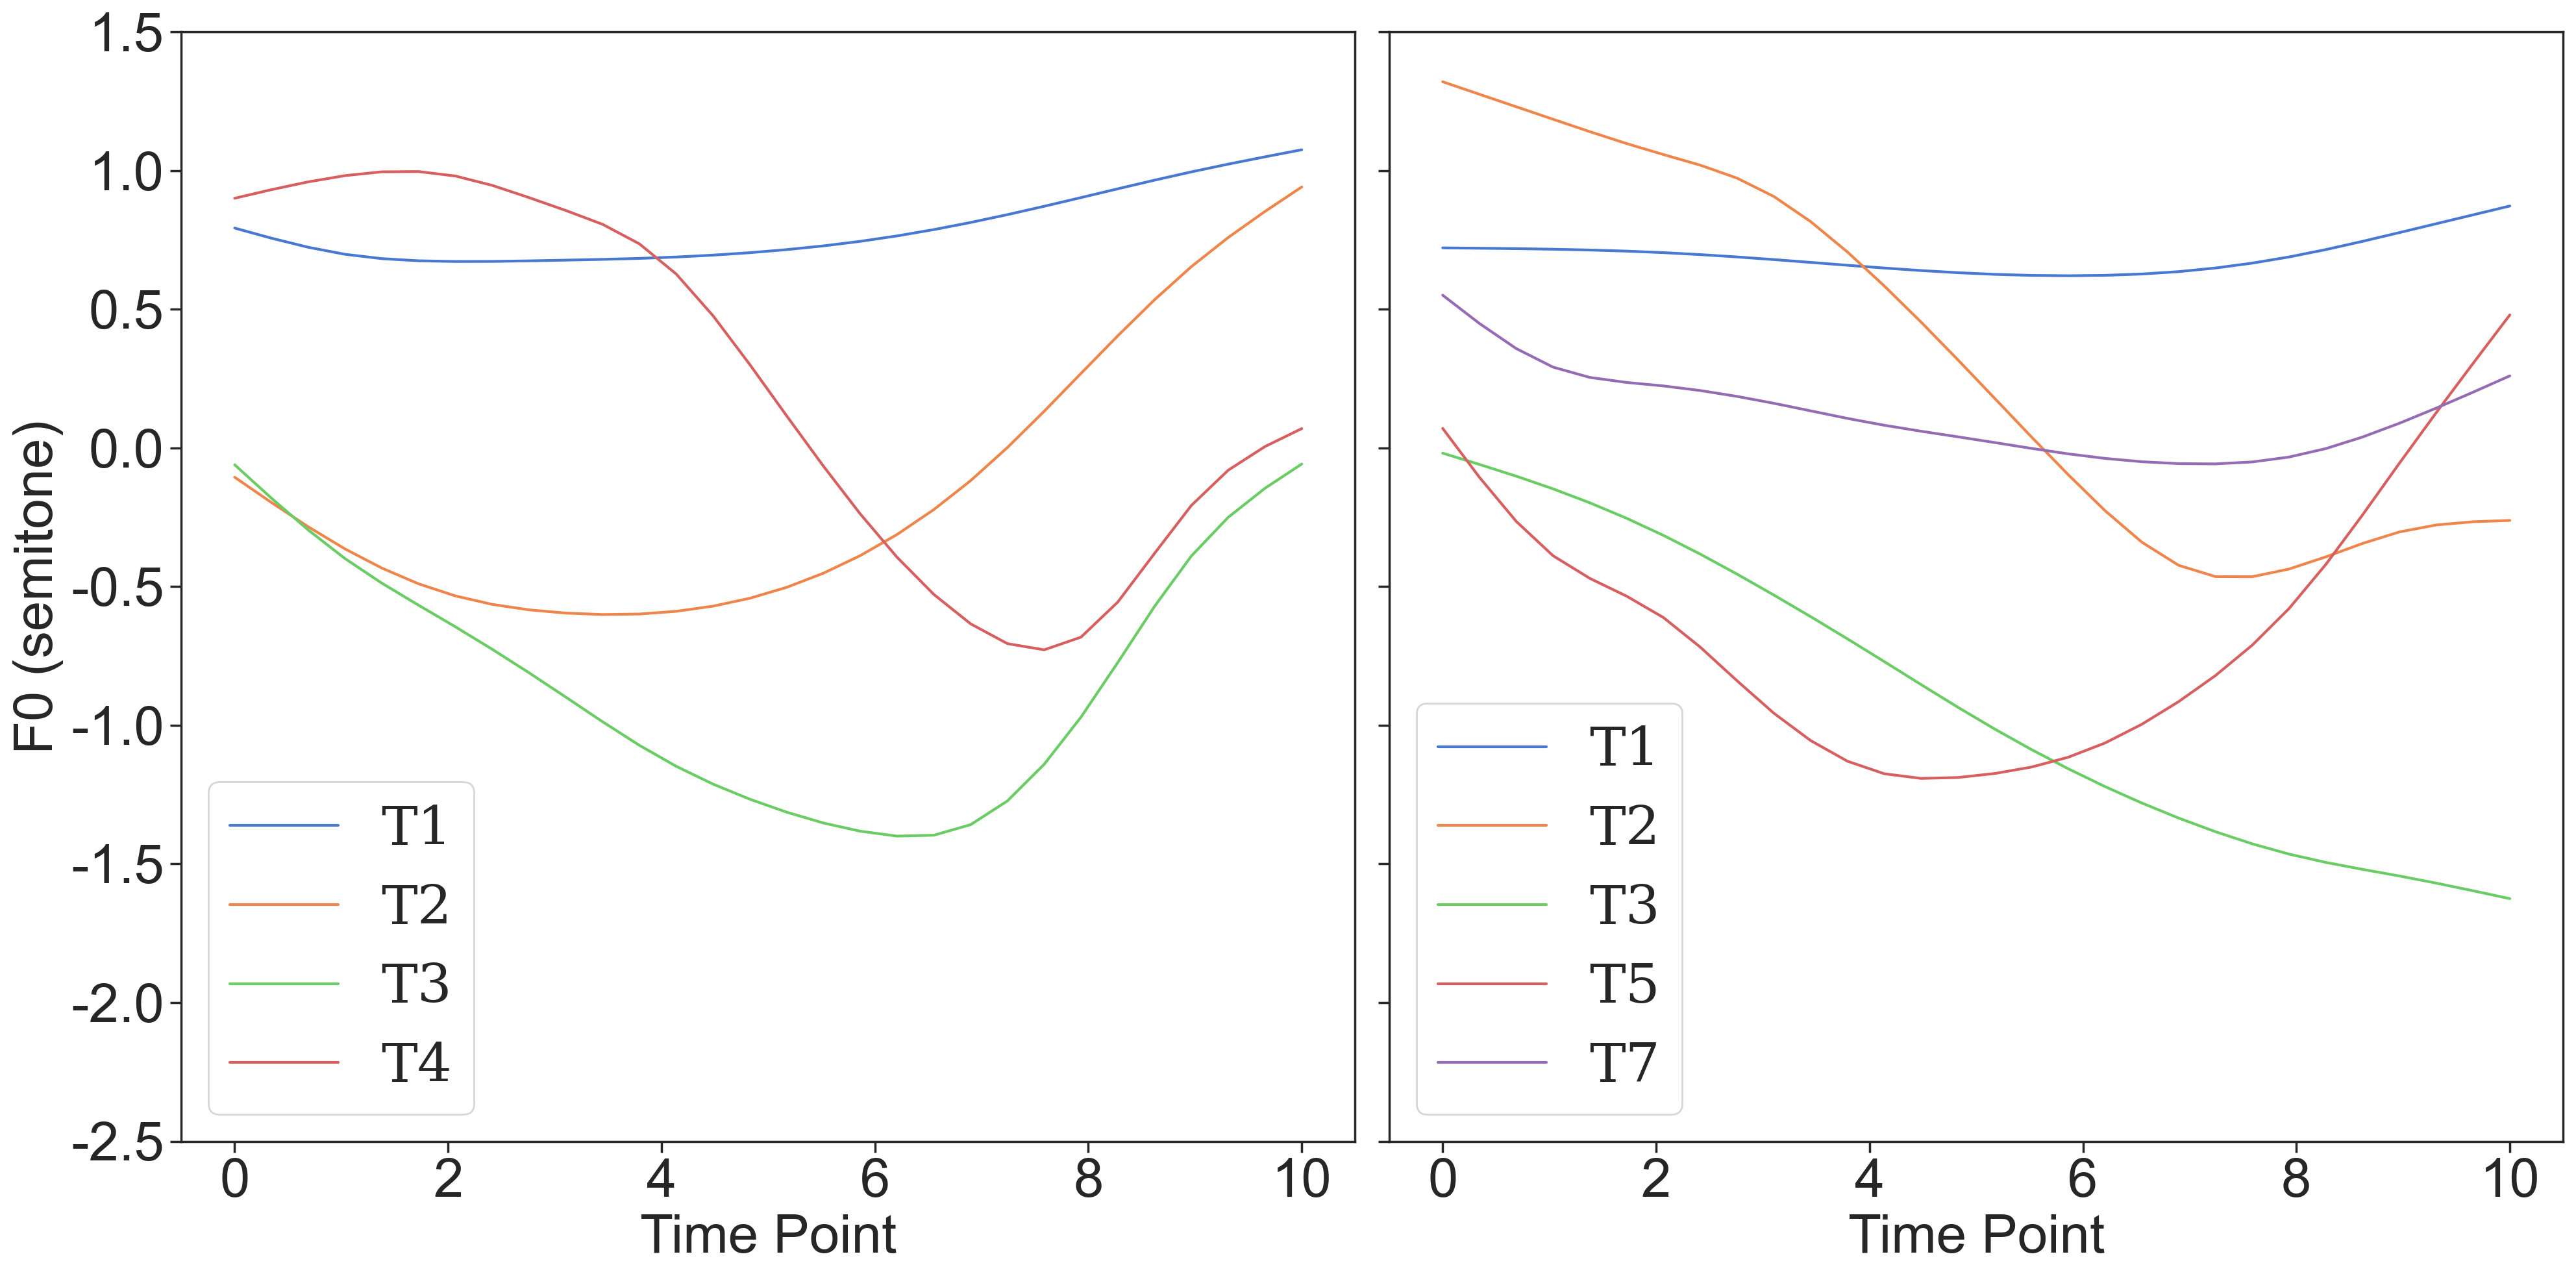
\includegraphics[scale=.3]{Figures/Mandarin_Min_tone_contours.png}
%\caption{Lexical tones in Taiwan Mandarin (left) and Taiwan Southern Min (right)}
%\label{Figure:MandarinMinTones}
%\end{figure}

The variation of one tone under coarticulation with ambient tones was first mentioned in \cite{Chao1968}, where he noted that Mandarin T2 (35) would become T1 when preceded by T1 (55) or T2 (35). While the phonological status of such tonal variation is doubted by some (e.g., \citealp{ShihSproat1992}; \citealp{Xu1994}), follow-up studies generally agree that such variation is acoustically present, and is asymmetric (cf. \citealp{Shen1990}, however, for opposite findings), with carry-over effects (the influence of preceding tones) being stronger and assimilatory, and anticipatory effects (the influence of following tones) being weaker and dissimilatory. A question naturally arises: if the acoustic reality of tones is so fussy, how do Mandarin speakers understand them? \cite{Xu1997} investigated this question and found that Mandarin speakers actually normalized for such tone variation. When a target tone was preceded by a high pitch offset, it was perceived as lower, and vice versa. In this case, a raised T2 (35), which became 55, would still likely be perceived as 35.

However, things might be complicated when we turn to Taiwan Southern Min. In Mandarin, there are only 4 tones, and each of them can be distinguished by either tone shape or tone value alone. In Taiwan Southern Min, nevertheless, there are three level tones (T1, T7, T3) that are contrasted only by tone value, and there are 7 tones in total. Intuitively, if the tonal variation is to be as strong as in Mandarin, perception would be much more painstaking. A realized 33 may well be a raised T3 (21), a true T7 (33), or a lowered T1 (55), and a surface T2 (51) may be acoustically very similar to both a raised T3 (21) or T7 (33), and that is only considering carry-over effects. Possible tonal variations in Taiwan Mandarin and Taiwan Southern Min are provided in table \ref{table:Probablevariations}. As we can see, even under tonal coarticulation, the probable allotones in Mandarin still have a general one-to-one relationship, while the same Taiwan Southern Min tones may have multiple correspondences under coarticulatory effects. It is therefore presumable that tonal coarticulation in Taiwan Southern Min might be different from that in Taiwan Mandarin, and the way its speakers deal with such variation may also be different.

\begin{flushleft}
\begin{table}[hbt!]
\begin{tabularx}{\textwidth}{ll|X|X|X|X|}
\hhline{~~----}
 & & T1 (55) & T2 (35) & T3 (21(4)) & T4 (51)\\
\hhline{~~|----}\noalign{\vspace*{\doublerulesep}}
\hhline{--||----}
\multicolumn{1}{|l}{\multirow{2}{*}{Carry-over}} & \multicolumn{1}{l||}{Raised} & - & T1 (55) & T4 (51) & -\\
\multicolumn{1}{|l}{}& \multicolumn{1}{l||}{Lowered} & T2 (35) & - & - & T3 (21)\\
\hhline{--||----}
\multicolumn{1}{|l}{\multirow{2}{*}{Anticipatory}} & \multicolumn{1}{l||}{Raised} & - & - & T2 (35) & T1 (55) \\
\multicolumn{1}{|l}{}& \multicolumn{1}{l||}{Lowered} & T4 (51) & T3 (214) & - & -\\
\hhline{--||----}
\end{tabularx}
\break
\break
\begin{tabularx}{\textwidth}{ll|X|X|X|X|X|}
\hhline{~~-----}
 & & T1/T2' (55) & T2/T3' (51) & T3/T7' (21) & T5 (35) & T7/T1' (33)\\
\hhline{~~|-----}\noalign{\vspace*{\doublerulesep}}
\hhline{--||-----}
\multicolumn{1}{|l}{\multirow{2}{*}{Carry-over}} & \multicolumn{1}{l||}{Raised} & - & - & T7 (33); T2 (51) & T1 (55) & T1 (55); T2 (51)\\
\multicolumn{1}{|l}{}& \multicolumn{1}{l||}{Lowered} & T5 (35); T7 (33) & T7 (33); T3 (21) & - & - & T3 (21)\\
\hhline{--||-----}
\multicolumn{1}{|l}{\multirow{2}{*}{Anticipatory}} & \multicolumn{1}{l||}{Raised} & - & T2' (55) & T1' (33) & - & T2' (55) \\
\multicolumn{1}{|l}{}& \multicolumn{1}{l||}{Lowered} & T1' (33); T3' (51) & - & - & T1' (33) & T7' (21)\\
\hhline{--||-----}
\end{tabularx}
\caption{Probable variations of Taiwan Mandarin (top) and Taiwan Southern Min (bottom) lexical tones under types of coarticulation}
\label{table:Probablevariations}
\end{table}
\end{flushleft}

Indeed, past studies in (Taiwan) Southern Min tonal coarticulation yielded rather different results from what we have seen in (Taiwan) Mandarin. While \cite{Peng1997} and \cite{Wang2002} found anticipatory (Peng and Wang) and carry-over (Wang) effects in Taiwan Southern Min, the effects were symmetric and both assimilatory, unlike the asymmetry attested in (Taiwan) Mandarin. Even, \cite{Lin1988} did not find significant coarticulatory effect in Taiwan Southern Min at all. \cite{ChangHsieh2012}, investigating the same issue in Malaysian Hokkien, a dialect of Southern Min, also found rather inconsistent results, where carry-over and anticipatory effects could be both assimilatory and dissimilatory. While the perception of tonal coarticulation may shed light on this issue, past researches on the perception of Taiwan Southern Min tonal coarticulation are rather sparse. To the author's knowledge, only \cite{Peng1997} and \cite{Wang2002} have investigated this issue. In \cite{Peng1997}, it was discovered that Taiwan Southern Min speakers had an above-chance identification rate of identical syllables followed by different tones even when they were truncated from the original words, which was taken as proof that tonal coarticulation was salient enough to be detected in perception. \cite{Wang2002} also found that tone identification rates were influenced when the ambient tones were swapped, though the results were inconsistent.

Overall it is likely tonal coarticulations in Taiwan Mandarin and Taiwan Southern Min are different, and the normalizing mechanisms of the speakers of the two languages to cope with tone variation are also possibly rather different. However, since no study so far have investigated and compared the tonal coarticulations of two different tone languages, and the experiment designs, materials used, and the goals of past studies were all different, a direct comparison between two languages is difficult. This paper thus aims to compare the production and perceptual normalization of tonal coarticulations in Taiwan Mandarin and Taiwan Southern Min with systematic and quantifiable designs. Crucially, the following questions are asked: 1) Are carry-over effects of tonal coarticulation of the same magnitude in both Taiwan Mandarin and Taiwan Southern Min? 2) If carry-over effects are of different magnitudes in these two languages, how may speakers of these two languages behave differently in the normalization for tonal coarticulation? 3) If the effects are equally strong in both languages, how then, do Taiwan Southern Min users cope with the possible confusions of lexical tones? One stipulation would be that Taiwan Southern Min does not have such strong tonal coarticulation as in Mandarin, and therefore would not need to compensate for such variation. Another possibility would be that while Taiwan Southern Min does have tonal coarticulation, Taiwan Southern Min users have stricter boundaries between the lexical tones, and therefore would not easily perceive a raised/lowered tone as other tones. The last scenario would be that both the production of coarticulated tones and their perception are identical in both Mandarin and Taiwan Southern Min, and that Taiwan Southern Min speakers have to result to other means such as lexicons to enable effective communication. These three scenarios are illustrated in figure \ref{Figure:ThreePossibleScenarios} as routes C, B, and A respectively. Among the three, routes B and C are not likely to lead to normalization, as the lexical tones are not perceived phonemically as other tones to start with, and therefore no compensation is in need. In route A, additional normalization will be likely since coarticulatorily -raised/-lowered tones are phonmeically recognized as other tones, and listeners may make correction based on the acknowledgement of such variation. Such a route, however, might be less probable in languages with larger inventories of lexical tones, since speakers may not know to what extent they should make the compensation. In Mandarin, a phonetically-realized high falling tone can be reasonably normalized back as a raised 21, while in Southern Min, the options can be both a raised 21 or a distorted 33. While Mandarin listeners need only know that the tone is raise, Southern Min listeners not only have to know that it is raised, but also how much, in order to facilitate faithful normalization.

\begin{figure}[hbt!]
\centering
\begin{tikzpicture}
\node [terminator] at (5,0) (block1) {Tone production};

\node [terminator] at (0,-2) (block2_1) {Strong tonal coarticulation};
\node [terminator] at (10,-2) (block2_2) {Weak tonal coarticulaiton};

\node [terminator] at (5,-4) (block3) {Phonetic-level perception};

\node [terminator] at (0,-6) (block4_1) {Loose tonal boundaries};
\node [terminator] at (5,-6) (block4_2) {Strict tonal boundaries};

\node [terminator] at (5,-8) (block5) {Phonemic-level perception};

\node [terminator] at (5,-10) (block6) {Normalization};

\node[draw=none] at (10-.3, -5) (text_1) {C};
\node[draw=none] at (0-.3, -5) (text_2) {A};
\node[draw=none] at (5-.3, -5) (text_3) {B};

\path [connector, color={rgb,255: red, 76; green, 0; blue, 153}] (block1) -| (block2_1);
\path [connector, color={rgb,255: red, 76; green, 153; blue, 0}] (block1) -| (block2_2);

\path [connector, color={rgb,255: red, 76; green, 0; blue, 153}] (block2_1) -- (block3);
\path [connector, color={rgb,255: red, 76; green, 153; blue, 0}] (block2_2) -- (block3);

\path [connector, color={rgb,255: red, 204; green, 0; blue, 0}] (block3) -| (block4_1);
\path [connector, color={rgb,255: red, 0; green, 128; blue, 255}] (block3) -- (block4_2);
\path [connector, color={rgb,255: red, 76; green, 153; blue, 0}] (block3.east) -- (10, -4)|-(block5);


\path [connector, color={rgb,255: red, 204; green, 0; blue, 0}] (block4_1) |- (block5);
\path [connector, color={rgb,255: red, 0; green, 128; blue, 255}] (block4_2) -- (block5);

\path [connector, color={rgb,255: red, 204; green, 0; blue, 0}] (block5) -- (block6);

\end{tikzpicture}
\caption{Three possible scenarios of tone perception under tonal coarticulation}
\label{Figure:ThreePossibleScenarios}
\end{figure}


In the next chapter, we shall first take a more detailed look at tonal coarticulation in (Taiwan) Mandarin and (Taiwan) Southern Min. We then review how tonal coarticulation is perceived in these two languages. In chapter 3, we talk about the experiment designs, data processing and analyses, and test results.

%===Backgrounds===
\pagebreak
\chapter{Background}

In this chapter, we shall review past studies on the production of and the normalization for tonal coarticulation in Taiwan Mandarin and Taiwan Southern Min. 
\section{Tonal coarticulation in Taiwan Mandarin and Taiwan Southern Min}\label{section:Tonal coarticulation in Taiwan Mandarin and Taiwan Southern Min}
In this section, we introduce tonal coarticulation, which refers to the tone variation caused by the preceding/following tones, in Taiwan Mandarin and Taiwan Southern Min. Typological findings generally agree on an asymmetric directionality of tonal coarticulation \citep{ChangHsieh2012}, with carry-over effects being strong and assimilatory and anticipatory effects being weak and dissimilatory. This is illustrated in table \ref{table:Typologicaldistribution}.

\begin{flushleft}
\begin{table}[hbt!]
\begin{tabularx}{\textwidth}{l|X|X|}
\hhline{~--}
 & Magnitude & Direction \\
\hhline{~|--}\noalign{\vspace*{\doublerulesep}}
\hhline{-||--}
\multicolumn{1}{|l||}{Carry-over} & Strong & Assimilatory\\
\hhline{-||--}
\multicolumn{1}{|l||}{Anticipatory} & Weak & Dissimilatory\\
\hhline{-||--}
\end{tabularx}
\caption{Typological distribution of tonal coarticulation}
\label{table:Typologicaldistribution}
\end{table}
\end{flushleft}

While production studies of Mandarin tones seem to support such distribution, both the presence and distribution of tonal coarticulation in Taiwan Southern Min is lacking consensus in the literature. For the remainder of this section, we shall go through past studies on the production of tonal coarticulation in these two languages.

\section{Tonal coarticulation in Taiwan Mandarin}
Following \cite{Chao1968}, several studies have been conducted in attempt to measure tonal coarticulation in Mandarin.

\cite{ShihSproat1992} measured the pitch height of T1 (55)-T2 (35)-T1 (55) and all T1 (55) trisyllabic words in isolation, read sentences, and conversation, and found that the pitch contour flattened as it went from being in isolation to in conversation. The authors found a general positive correlation between the amounts of F0 displacement and the duration of the words. This correlation, however, was weak within the read sentence and conversation groups. The authors additionally looked into quadrisyllabic words where T2 (35) was either in the second (weak) syllable or the third (strong) syllable, and it was found that F0 displacement was lower in weak syllables than in strong syllables. The authors therefore concluded that prosodic stress was the primary reason for Chao's T2-T1 tone variation rule.

A more holistic study on the coarticulation of Mandarin tones was conducted in \cite{Shen1990}, where trisyllabic non-words /\tip{pa.pa.pa}/ with combinatorial tone combinations were used as test materials. Subjects were asked to pace themselves so the three syllables were of the same durations.  She found that tone variation along with surrounding tones was not exclusive to T2 (35) but was applied to all tone combinations, to varying degrees, and unlike the typological distribution, these effects were symmetric, and affect not only part, but the whole syllable. It was also noticed that such coarticulatory effect only affects the tone values, but not the direction of the tones. Crucially, T2 (35) was found to raise its adjacent tones the most, followed by T1 (55), while T3 (21) effectively lowered their following tones. T4 (51) also lowered its following tones, but did not raise its preceding tones as mush as T1 (55) or T2 (35).

\cite{Xu1994} additionally investigated Mandarin rising tone and falling tone in compatible (i.e., low offset before and high onset after the rising tone, and high offset before and low onset after the falling tone) contexts and conflicting (i.e., opposite directions as the compatible contexts) contexts, and found that rising tones were slightly falling in conflicting contexts, and that falling tones were less steep in such contexts. This was rather different from \cite{Shen1990}, where tone movements were invariable and only F0 values were affected.

More results supporting an asymmetric distribution were borne out in \citeauthor{Xu1994a} (\citeyear{Xu1994a}, \citeyear{Xu1997}), where disyllabic syllables of /\tip{ma.ma}/ of tone combinations in carrier sentences with different pitch onsets/offsets were measured. Like \cite{Shen1990}, Xu found coarticulatory effects from both preceding and following tones. What was different was that the anticipatory effects found in \citeauthor{Xu1994a} (\citeyear{Xu1994a}, \citeyear{Xu1997}) were dissimilatory in nature, and the magnitude was also much weaker.

An asymmetry of tonal coarticulation was also found in \cite{LinYan1991}, who also measured quadrisyllabic words, and found that tonal coarticulation in Mandarin was unidirectional, that is, each tone was under either carry-over or anticipatory effect.

Another inconsistency in the literature was that while \cite{Shen1990} and \citeauthor{Xu1994a} (\citeyear{Xu1994a}, \citeyear{Xu1997}) both found that coarticulatory effects could affect as large as the whole adjacent syllable, \cite{LinYan1991} noted that such effects would fade and did not span across the syllable.

Overall, the literature seems to support an asymmetric distribution of Mandarin tonal coarticulation, though inconsistencies exist.

\section{Tonal coarticulation in Taiwan Southern Min}
While past studies on tonal coarticulation in (Taiwan) Mandarin were plenty, much fewer related works can be found in (Taiwan) Southern Min. One of them is \cite{Peng1997}, where the syllables /\tip{kaw}/ of different tones followed by a high- (55), mid- (33) or low- (21) level tone in phrase -initial, -medial, and -final and utterance-final positions were used as materials, and produced by 4 (2 females) Taiwan Southern Min native speakers. Both prosodic positions, tonal contexts, and their interactions were found to have significant effects on tone variations. Crucially, the coarticulatory effects (i.e., anticipatory effects) were mostly assimilatory, contrary to what we see in Mandarin and typology. An identification test also showed that the subjects could detect such coarticulatory effect. In the identification test, the target syllables /\tip{kau}/ were exercised from the original sentences produced by one of the female subjects, and subjects were asked to guess which syllable the exercised syllable was. The subjects achieved an above-chance identification rate. This was taken by the author as proof that such anticipatory coarticulation was salient enough to be detected by the subjects. It should be noted, however, that  the materials used in these two experiments were sentential, and that one of the main aims of this study was to measure the prosodic effect on tone variation. It is therefore hard to assess to which extent the prosodic effect was at work and how it might have interacted with tonal contexts in sentence production. Crucially, the materials used in the identification test were not synthesized; the duration, prosody, and intensity were all retained. Since tones have intrinsic durations, and other suprasegmental properties may also give hints to the listeners, it seems audacious to assert such results were directly associated with tonal coarticulation.

Two more comprehensive works that studied both the anticipatory and carry-over effects were \cite{Lin1988} and \cite{Wang2002}. In \cite{Lin1988}, Taiwan Southern Min Tones in isolation and in sequence were measured. Though small carry-over effect was observed, the author found generally no much coarticulatory effect in Taiwan Southern Min. This is in contradiction with \cite{Wang2002}, where trisyllabic non-words, with T1' (55)/T7' (21) as the first syllables, T2' (55)/T1' (33)/T7' (21) as the second syllables, and T5 (24)/T2 (51) as the last syllable, were used as test materials. 6 male college students participated in the production. Partial significance of stronger carry-over and weaker anticipatory effects were found between some pairs. It should be noted, however, that the subjects were Taiwanese college students at the 2000s, it is presumable that they were very likely also native in Mandarin, and the words used were non-words, with all the tones except T1' (33) also present in Mandarin. Therefore, there is virtually no knowing to what extent these non-words could be perceived as Taiwan Southern Min by the subjects, and whether their production was influenced by Mandarin. \cite{ShihSproat1992} also noted that Mandarin non-words induced different coarticulatory effects than did real words. It is possible that tonal coarticulation would have different distribution between non-words and real words.

Finally, another related work, \cite{ChangHsieh2012}, which investigated tonal coarticulation in Malaysian Hokkien, a dialect of Southern Min, looked into monosyllables and disyllables. Disyllables were grouped into higher/lower onset/offset groups to compare anticipatory and carry-over effects. Two types of grouping were used: one with the tonal scales, where tone values with 3 or above were categorized as higher, and with 2 or below as lower; the other one used the centroid of the tones as the threshold. The first kind of grouping yielded virtually no significant coarticulatory effect in Malaysian Hokkien, while significant, but mixed effects were found in the second grouping, where both the carry-over and anticipatory effects could be assimilatory or dissimilatory.

Overall, past studies in the literature have rather inconsistent results regarding tonal coarticulation in (Taiwan) Southern Min. This may well be due to the different research goals, test materials, statistical quantifications, and different dialects studied.

\subsection{Section summary}

In this section, we reviewed tonal coarticulation in (Taiwan) Mandarin and (Taiwan) Southern Min. Discrepancies exist among the literature. Crucially, while most studies agree tonal coarticulation in (Taiwan) Mandarin exists and is asymmetric, a consensus regarding this issue is lacking in (Taiwan) Southern Min. A cross-linguistic comparison will therefore require a consistent and quantifiable experiment design.

\section{Normalization and tonal coarticulation normalization in Taiwan Mandarin and Taiwan Southern Min}

In this section, we shall first briefly discuss perceptual compensation/normalization in general, including the two major kinds of normalization, and the issue of whether and to what extent normalization is speech-specific. For the second half of this section, we will discuss past studies on the normalization of tonal coarticulations in (Taiwan) Mandarin and Taiwan Southern Min.

\subsection{Kinds of normalization and the speech-specificity of normalization}

Speech is built on the production and perception of phonetic categories including both segmental and suprasegmental elements. The acoustics of speech in real-life circumstances, however, are highly variable, subject to factors such as talker differences (e.g., the morphology of vocal tracts due to sex, age, and race; \citealp{Markovaetal2016}), acoustic effects of adjacent sounds, or the physical environment in which the speech takes place. These variances can be further categorized into two major types: inter-talker variances, and intra-talker variances \citep{Francisetal2003}. The former includes the formant and pitch range differences caused by the size of vocal tracts, larynxes and morphology of vocal folds \citep{JohnsonSjerps2018}, and individual speech styles. The latter refers to the variances of the same phonological elements within the same speaker. This may be caused by factors such as coarticulation with ambient sounds (\citealp{WangFillmore1961}), the prosodic location of the target element (e.g., \citealp{Peng1997}), or the register of the speaker at the moment of speech (e.g., \citealp{Schaferetal2000}). Tonal coarticulation in this sense is a kind of intra-talker variance.

In order for a speech to be successful, listeners have to make accommodations for such acoustic variances. These accommodations are commonly referred to as ``normalizations'' or ``perceptual compensations'' (cf. \cite{Zhangetal2022} for a more detailed distinction of terminology; in this paper, we follow the conventional ``normalization''). Normalization according to the types of variance, can be inter-talker normalization (or simply talker normalization) or intra-talker normalization (which includes tonal coarticulation normalization). Such theme was first explored in \cite{LadefogedBroadbent1957}, where the authors investigated the perception of four English vowels /\tip{I}/, /\tip{E}/, /\tip{5}/, /\tip{2}/ in the words \textit{bit}, \textit{bet}, \textit{bat}, and \textit{but}, preceded by 6 introduction sentences with varying F1's and/or F2's. Their results showed that acoustically identical tokens were perceived as different words when followed by sentences with different F1-F2 spaces. This suggests that in perception, listeners do not only blindly follow the intrinsic acoustics of the sounds, but make use of extrinsic cues and make normalization accordingly.

Such talker normalization is also found for suprasegmental elements such as the perception of tones. \cite{WongDiehl2003} investigated the tone perception of Cantonese level tones on three monosyllabic words /\tip{si}1/ `teacher', /\tip{si}3/ `to try', and /\tip{si}6/ `yes', with T1, T3, and T6 being respectively high-, mid-, and low- level tones, and found that the identification rates were significantly higher in talker-blocked conditions than when the talkers were mixed within the same block. In addition, such talker normalization was found to change the categorization of level tones when they were preceded by contexts with higher/lower F0's. Contexts with 2 semitones higher than the neutral contexts were found to lower the perceived F0 of the target tones, leading all three words to be identified as /\tip{si}6/, and contexts with 2 semitones lower raised the perceived F0 of the following words, which were identified as /\tip{si}1/. 

However, several studies have put this kind of speech-specific stance into question, suggesting that what is viewed as normalization is but a general cognitive process that can be induced by even non-speech contexts. \citeauthor{WatkinsMakin1994} (\citeyear{WatkinsMakin1994}; \citeyear{WatkinsMakin1996}) imitated the experiment design of \cite{LadefogedBroadbent1957}, but substituted the introduction sentences with non-speech materials, and still successfully induced similar perceptual compensation. 

In sections 2.2 and 2.3, we will look at tone normalization, including inter-talker normalization and normalization for tonal coarticulation, and show that judging from past studies, normalization, at least that of tone, is not purely speech-irrelevant, and thus might be affected by language-specific variables.

\subsection{Intra-talker tone normalization and tonal coarticulation normalization in Taiwan Mandarin and Taiwan Southern Min}

As seen in section 2.1, inter-talker normalization is found not only for segments but also for tones, such as in Cantonese \citep{WongDiehl2003}. This phenomenon is also attested in Mandarin. In \cite{HuangHolt2009}, a T1-T2 continuum, with T1 being a high-level (55) tone, and T2 a mid-rising (35) tone, as the targets were preceded by two context sentences, one with an average F0 of 200 Hz, and the other with an average F0 of 165 Hz. They found that higher context sentences shifted the T1-T2 threshold backward as the targets went from mid-rising to high-level, suggesting that higher-F0 contexts also lowered the perceived F0 of the targets. 

Similar results were borne out in tonal coarticulation normalization in Mandarin. \cite{Xu1994} examined the identification of target T2 (25) and T4 (51) tones with the original preceding tones swapped with higher-/lower- offset tones in trisyllabic non-words. While identification rates were similar in compatible sequences (cf. section 1.1), the identification rates in conflicting sequences were found to be significantly lower when the tones were swapped. In addition, \cite{Zhangetal2022}, by creating a continuum from T3 (21) to T4 (51), preceded by T1 (55), T2 (35) and T4 (51) with minimal contrasting pairs, also found that higher preceding offsets shifted the perception toward T3 (21), while when the first syllables had lower tone offsets, the targets were more easily perceived as T4 (51).

Related works in Taiwan Southern Min, again are sparse. \cite{Wang2002}, however, did report certain effect of normalization of Taiwan Southern Min tonal coarticulation. The author swapped tones in Taiwan Southern Min trisyllables produced by one of the subjects in the production experiment mentioned in section 1.2, and found that T2' (55) and T1' (33) seemed to be perceived as lower when preceded by higher offsets, and vice versa. The results were not systematic, though. In addition, the author only reported a general significant effect of tone swapping on identification rates. It is hard to tell exactly what kind of effect (i.e., the directionality) it was, and since the measurement was the identification frequency, systematic quantification would be difficult. Crucially, the stimuli were not synthesized, and were non-words. The same issue mentioned in section 1.2 regarding \citeauthor{Peng1997}'s (\citeyear{Peng1997}) identification test design and this author's production test would also happen.

However, if we are to compare normalization of tonal coarticulation between Taiwan Mandarin and Taiwan Southern Min, we shall first address the issue of whether normalization is speech-specific or is simply a general perceptual process. If it is a general perceptual process, immediately there would be no need for such cross-linguistic comparison, since it is not reserved for language in the first place.

The theme of speech-specificity of tone normalization was explored in \cite{HuangHolt2009} and \cite{Zhangetal2022}. In the former, aside from using context sentences of high/low mean F0's, the authors also used pure tones as preceding contexts. Similar results were seen both when the preceding contexts were sentences and when they were non-speech. \cite{Zhangetal2022} also found that non-speech preceding syllables could elicit similar effects as could speech syllables, only to a much lesser degree. \cite{Zhangetal2022} therefore stipulated that tone normalization had both general perceptual processes and other factors involved, which contributed to the larger effect seen for the speech group versus the non-speech group. Why this difference in magnitude was not seen in \cite{HuangHolt2009} could be due to the smaller F0 difference between the context materials \citep{Zhangetal2022}.

Overall, we shall conclude that while tone normalization may be partially due to general cognition, speech-specificity, and therefore language-specificity, may also be present.

\subsection{Section summary}
In this section we reviewed past studies on normalization, inter-talker tone normalization and, more importantly, tonal coarticulation normalization. It is found that both Taiwan Mandarin and Taiwan Southern Min tone production may be subject to the normalization of coarticulation, though a direct comparison is not possible with the studies at hand.

\section{Summary}
Discrepancies exist in the results of tonal coarticulation and the normalization of it in (Taiwan) Mandarin and (Taiwan) Southern Min. Specifically, no study have systematically compared tonal coarticulation in two languages with different tone systems, and a quantifiable test for measuring tonal coarticulation normalization in the two languages, especially Taiwan Southern Min is lacking. This study therefore hopes to fill in this gap with a cross-linguistic comparable design. In the next chapter, we shall talk about the three experiments conducted in this study.

%===Methods===

\pagebreak
\chapter{Methods}

In this chapter, we will talk about the experiments conducted in this study, including the experiment designs, data processing, analyses, results, and discussions. The first experiment is a production task that measures both carry-over and anticipatory effects in Taiwan Mandarin and Taiwan Southern Min. The second experiment is a replication of \cite{Zhangetal2022}, where the magnitude of normalization of tonal coarticulation is measured. The last is a word-non-word test, aiming to examine how strict the subjects were on the tone boundaries.


\section{Experiment 1}
Experiment 1 measures tone productions in monosyllabic and disyllabic words in Taiwan Mandarin and Taiwan Southern Min. This experiment seeks to reexamine the magnitudes and behaviors of tonal coarticulations in these two languages.

While it is established in the literature that the pitch values of Mandarin tones are subject to those of their preceding (carry-over effects) and following tones (anticipatory effects), with carry-over effects being stronger and assimilatory, and anticipatory effects being weaker and generally dissimilatory, studies on tonal coarticulation in (Taiwan) Southern Min lead to less consistent results: while \cite{Peng1997} finds anticipatory tonal coarticulation in Taiwan Southern Min, and \cite{Wang2002} stronger carry-over effects and weaker anticipatory effects, \cite{ChangHsieh2012} finds inconsistent assimilatory and dissimilatory effects for both carry-over and anticipatory coarticulations. This may be due to the different experiment designs and dialects examined: in \cite{Wang2002}, non-words were used as stimuli, with syllables also found in Taiwan Mandarin. Such design may lead the speakers to be influenced by Mandarin, in which they were presumably also native; in \cite{ChangHsieh2012}, it is Malaysian Hokkien that was examined, while in \cite{Peng1997} and \cite{Wang2002}, it was Taiwan Southern Min. A reexamination with a consistent design is thus in need if we are to compare tonal coarticulations in these two languages, and to observe how the differences in tonal coarticulations may exert different effects on the way the speakers compensate for them perceptually.

\subsection{Participants}

This study recruited 43 Taiwanese college students (25 females; 20–27 y.o., mean=21.93) as participants. 15 of them were native speakers of Taiwan Mandarin. These subjects were not speakers of Taiwan Southern Min (upon self-report). These speakers are hereafter refereed to as the monolingual group. 28 of them were native speakers of Taiwan Southern Min. These subjects were also speakers of Taiwan Mandarin. These speakers will be referred to as the bilingual group. Among the bilingual speakers, 11 speakers were advanced Taiwan Southern Min speakers, with self-reported points of 8 or higher on a fluency scale from 1–10. These 11 speakers will be referred to as the advanced bilingual group. The rest of the bilingual speakers will be referred to as the intermediate bilingual group. All of the subjects were not speakers of other tonal languages. See Appendix \ref{Appendix:ParticipantInfo} for a full list of the participants. 

For Experiment 1, only the monolingual speakers\footnote{Except for P22.} and the advanced bilingual speakers participated. The monolingual speakers produced the Mandarin stimuli; the bilingual speakers produced both the Southern Min and Mandarin stimuli.

\subsection{Stimuli}
To examine the influence of ambient tones on the target tones, a disyllabic word was chosen for each of the 16 (4 tones × 4 tones, for Taiwan Mandarin)/25 (5 tones × 5 tones\footnotemark, for Taiwan Southern Min) tone combinations as stimuli. Syllables with voiceless obstruents, affricates or fricatives were avoided. In addition, to observe the tones in neutral positions , 4 monosyllabic words with the 4 tones were chosen for Taiwan Mandarin group, and 7 monosyllabic words likewise for Taiwan Southern Min group. These resulted in a total of 20 words for Taiwan Mandarin group and 56 words for Taiwan Southern Min group, with 10 repetitions each. See Appendix \ref{Appendix:StimuliforExperiment1} for a full list of the stimuli.

\footnotetext{Check tones were excluded.}

\subsection{Apparatus}
The audio data were collected with a microphone (Audio–Technica Carcoid AT2035) plus a portable audio interface (USBPre 2), and saved as WAV files, with a sampling frequency of 44100 Hz.

\subsection{Procedure}
Subjects were first led through a list of the stimuli they would encounter, and made sure they are familiar with the words. The stimuli were then randomly presented on a MacBook Pro (13-inch, 2018) one at a time. For Taiwan Mandarin group, stimuli were presented in Traditional Chinese characters; for Taiwan Southern Min group, stimuli were presented in both Traditional Chinese characters and romanized forms, with their Mandarin glosses underneath. Subjects were asked to say the word when they saw it, at a relaxed pace. Subjects might press the button and proceed to the next word when they were ready. The stimuli were divided into two blocks, with a break in between. The whole process took about 10 minutes for Taiwan Mandarin group and 30 minutes for Taiwan Southern Min group. This experiment was done after Experiments 2 and 3.

\subsection{Data processing}
\subsubsection{Labeling}
The audio data were examined and processed with \textit{Praat} \citep{BoersmaWeenink2018}. Syllable boundaries were labeled and saved as \textit{Praat}’s TextGrid. Boundaries are determined with intensity and formant transition. A part of the TextGrids is shown below in figure \ref{Figure:TextGridExample}.

\begin{figure}[hbt!]
\centering
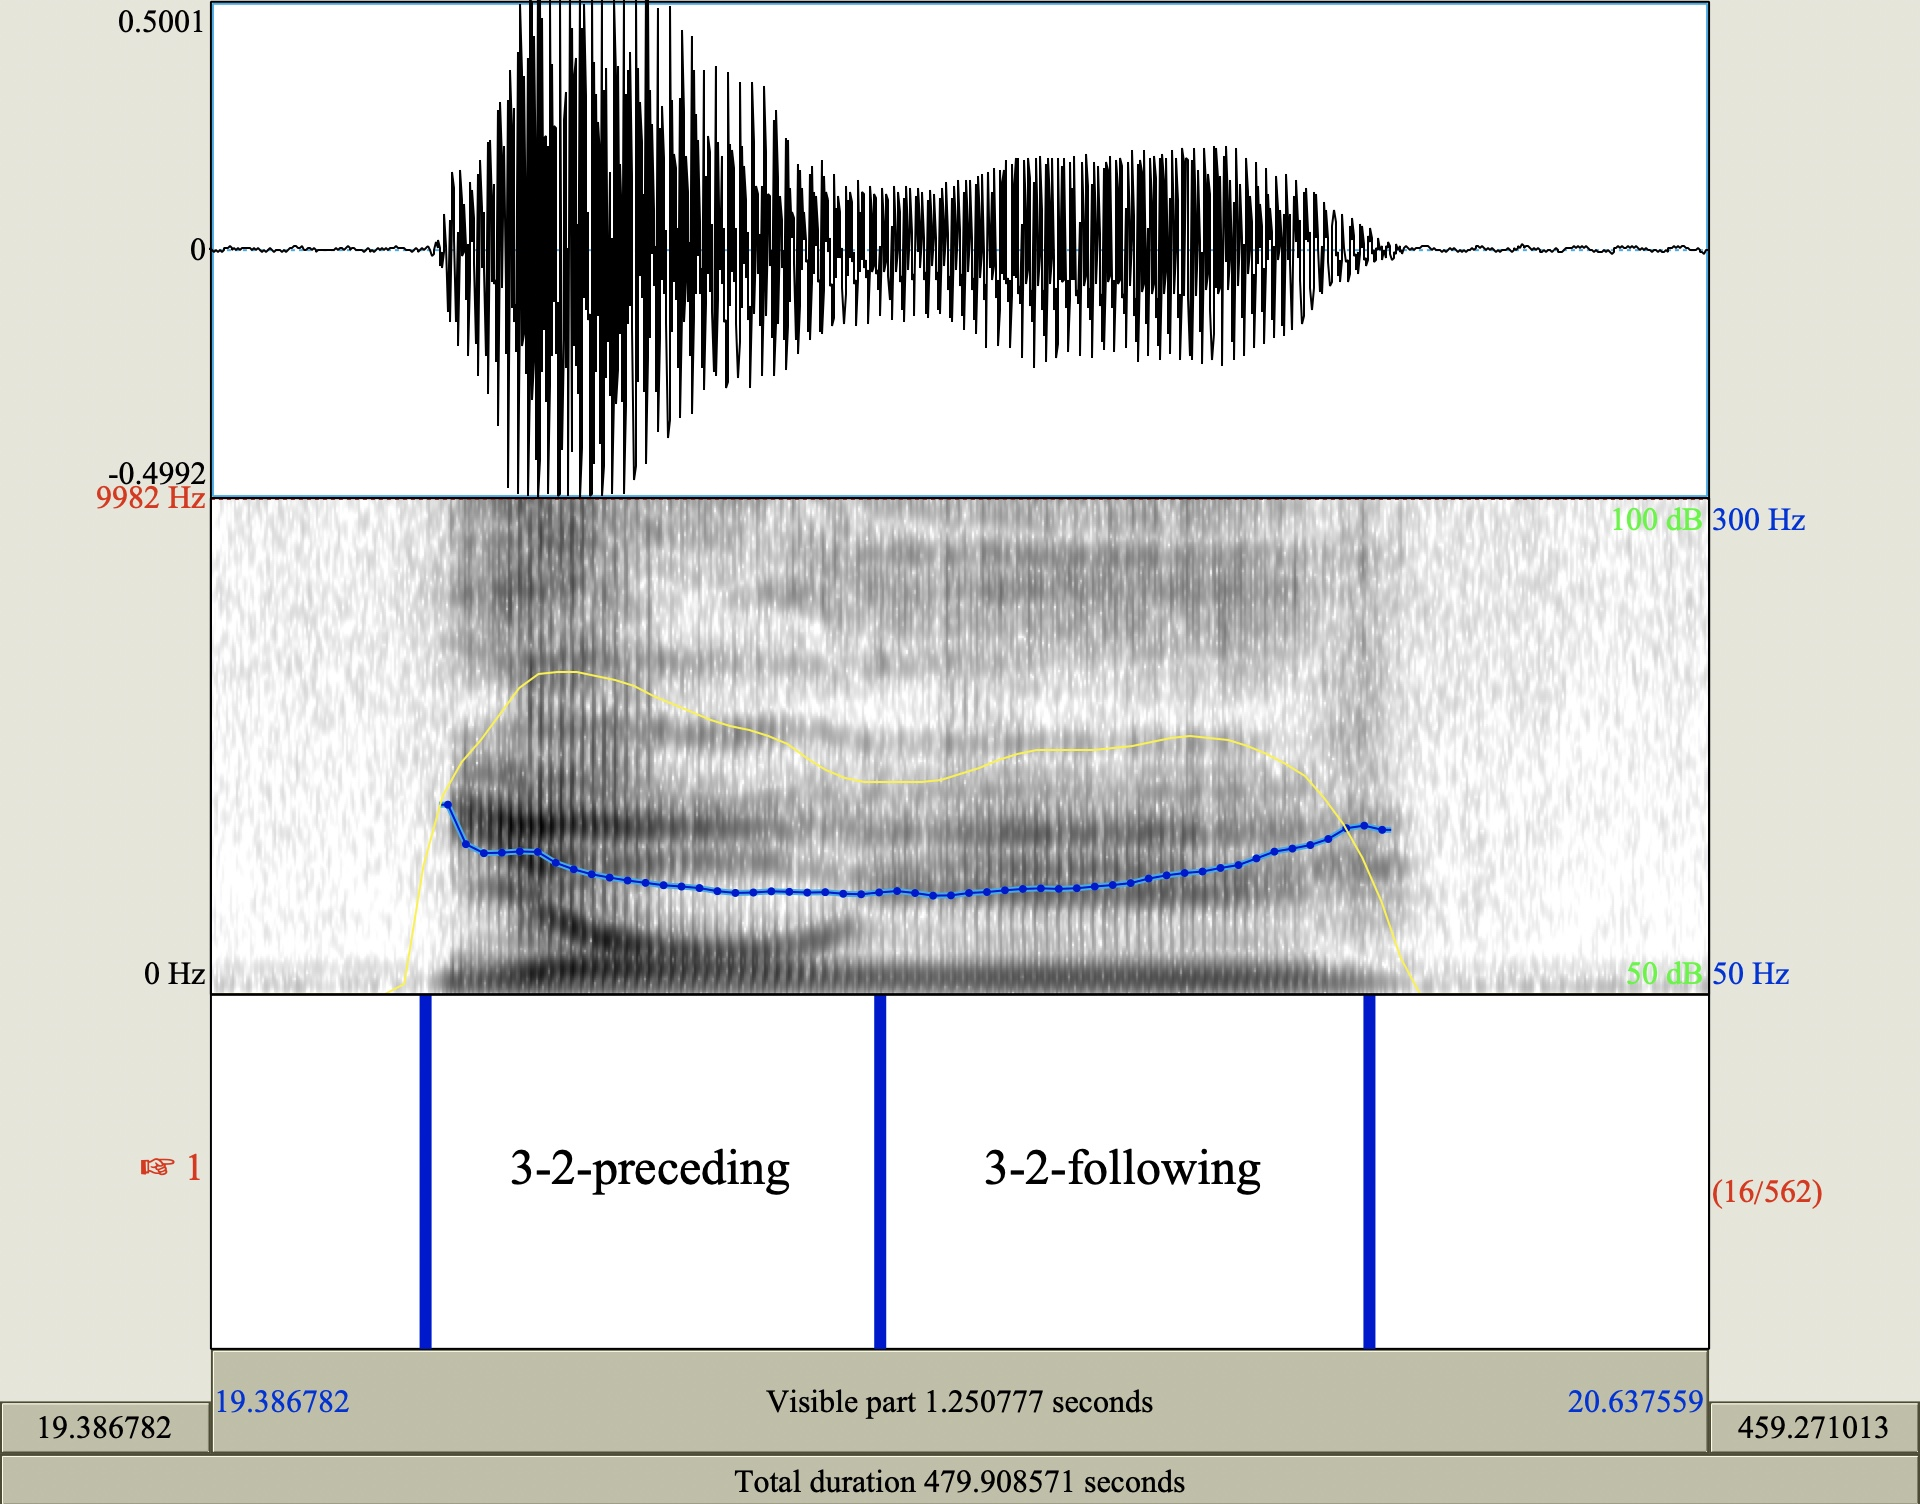
\includegraphics[scale=.45]{Figures/E1/TextGridExample.jpg}
\caption{Example of TextGrid labeling.}
\label{Figure:TextGridExample}
\end{figure}

\subsubsection{Pitch extraction}\label{section:PitchExtraction}
F0 values were extracted using \textit{Praat}, \textit{Parselmouth} \citep{Jadouletal2018}, and \textit{TextGridTools} \citep{BuschmeierWlodarczak2013} on Python 3.9 \citep{vanRossumDrake2009}. The time step was 0.01s. The pitch ceiling and floor values were determined individually for the each tone for each subject. To avoid possible failure to capture the F0 value for every time step, principally due to creaky voicing or extra-low pitch, for each tone production, the F0 values were divided into 11 proportions, missing values in a proportion were ignored, and the mean of the F0 values in each proportion was calculated. If all values in a proportion were missing, this proportion was discarded; if more than 3 of the 11 time points were discarded, this tone production was discarded. After all F0 values were extracted, they were converted to z-transformed semitones to make cross-subject comparison.

\subsection{Analyses}
\subsubsection{Pitch contour comparison}
For visualization and direct observation, F0 data were fitted through generalized additive mixed models (GAMMs; \citealp{Wieling2018}) with R Core \citep{RCoreTeam2019}’s \textit{lme4} package \citep{Batesetal2015}.

\subsubsection{Tonal coarticulation}
To quantify the magnitude of tonal coarticulation, the pitch onsets and offsets were first calculated. These were determined as the F0 means of the first and last 9.0\% (i.e. the first and last of the 11 time points mentioned in section \ref{section:PitchExtraction}) of each tone production, with missing values ignored. Linear mixed-effect models were fitted with R Core \citep{RCoreTeam2019}’s \textit{lme4} package \citep{Batesetal2015}. Several candidate models were compared according to their AIC scores. The chosen models had as the fixed effects the values of preceding offsets (in the case of carry-over coarticulation)/following onsets (in the case of anticipatory coarticulation, shown as \textit{x} in the code), language (Mandarin vs. Southern Min), and tones. Participants were taken as random inetrcepts, with a random slope of \textit{x} on each of level of \textit{participant}. The formula for carry-over coarticulation is provided below as an example\footnote{In the case of carry-over coarticulation, \textit{y} is the values of the following onsets}:

\begin{lstlisting}
    model <- lmer(y ~ x*language*tone + (x|participant))
\end{lstlisting}

In order to compare the magnitudes of carry-over and anticipatory effects within each of the two languages, other two models were fitted, with the fitted effects being the onset/offset values, positions (carry-over vs. anticipatory), and tones, and the same random effects as in the previous models.

\begin{lstlisting}
    model <- lmer(y ~ x*position*tone + (x|participant))
\end{lstlisting}

In this study, significant results (p<.05) were taken as indicator of existence of tonal coarticulation; positive coefficients were taken as indicator of assimilatory effects, and negative ones indicator of dissimilatory effects.

\section{Experiment 2}\label{section:Experiment2}
Experiment 2 measures the perceptual compensation for tonal coarticulation in Taiwan Mandarin and Taiwan Southern Min. Following the design of \cite{Zhangetal2022}, a continuum from low-level tone to falling tone preceded by tones of different pitch levels of offsets were synthesized into disyllabic stimuli, and subjects were asked to judge whether they hear a low-level tone or a falling tone. If perceptual compensation is at work, different pitch levels of preceding offsets should render different thresholds of low-level tone/falling tone judgement.

This experiment was divided into a Mandarin version and a Southern Min version.

\subsection{Participants}
All 41 participants participated in this experiment. The monolingual group did the Mandarin version. The bilingual group did both the Southern Min and Mandarin versions.

\subsection{Stimuli}
\subsubsection{Word selection}
3 Pairs of Taiwan Mandarin disyllabic words and 4 pairs of Taiwan Southern Min words were chosen for each of the two versions. These pairs were minimal pairs that differed only in the tones of the second syllables. Within each pair, the first syllables were the same and served as the primes, while the second syllables were the targets, and were a low-level tone and a falling tone, respectively. In this experiment, all tones in both languages that were suitable to serve as the primes were accounted for. In Taiwan Mandarin version, there were 3 pairs of words, with the primes (i.e., first syllables) of each pair being (55) (T1), 35 (T2) and 51 (T4), respectively, and the low-level tone being 21 (T3) and falling tone 51 (T4). The pairs were therefore T1+T3/T4, T2+T3/T4, T4+T3/T4. T3 as the primes were excluded due to tone sandhi. For Taiwan Southern Min version, 4 pairs of words were chosen, with the first syllables of each pair being 33 (T5'), 55 (T2'), 51 (T3'), and 21 (T7'), and the low-level tone being 21 (T3), and falling tone 51 (T2). The checked tones, 32 (T4'), and 54 (T8'), were excluded due to their inherently shorter durations. T1' was ignored since its value was the same as T5' (33) in the dialect we chose (the Southern dialect). 35 (T2') was also excluded since only the Quan dialect applies this sandhi rule. The pairs were thus T5'+T3/T2, T2'+T3/T2, T3'+T3/T2, T7'+T3/T2. See Appendix \ref{Appendix:StimuliforExperiment2} for the words used.

\subsubsection{Stimuli recording}
The words were produced by one male native speaker (25 y.o.) of Taiwan Mandarin and one male native speaker of Taiwan Southern Min (24 y.o.). The same apparatus used in Experiment 1 was used.

\subsubsection{Stimuli syntheses}
Following \cite{Zhangetal2022}, the stimuli were synthesized into continua where the pitch contours of the first syllables were made sure to be the same, and the pitch contours of the second syllables went from a low-level contour to a falling contour. The F0 values for the contours of the primes were converted from the five-level tone sacles with the equation of \cite{FonChiang1999}:
\[scale = \dfrac{1}{2}(39.86\times \log (\dfrac{f_{i}}{f_{min}})) + 1\] In this study, the $f_{min}$ was set at 100 Hz. This was approximately the natural pitch low point of the two speakers. The converted F0 values from scale 1 to 5 were: 100, 112.25, 125.99, 141.43, and 158.75 Hz. The starting F0 values of the targets were divided into 10 levels according on Bark's scale. The minimum was 0.9 and the maximum 1.9 on Bark's scale, with the step being 0.1. The end point was the minimum (0.9). The F0 values of this continuum in Hz were: 90.34, 101.59, 112.88, 124.2, 135.57, 146.99, 158.45, 169.97, 181.55, 193.19. The mean intensities of all syllables were scaled to be the same, and the durations of all syllables were 0.3 s. Illustrations of the synthesized pitch contours are given in figure \ref{Figure:SynthesizedToneContours}.

\begin{figure}[h]
\centering
\includegraphics[scale=.3, trim={0 8.5cm 0 0}]{Figures/E2/SynthesizedToneContours.png}
\caption{Illustrations of synthesized pitch contours (top: Taiwan Mandarin version; bottom: Taiwan Southern Min version).}
\label{Figure:SynthesizedToneContours}
\end{figure}

The audio data of the original disyllabic words produced by the two speakers were first exercised into separate syllables. The syllables's F0 values were then synthesized to match those presented in figure \ref{Figure:SynthesizedToneContours}. The durations and intensities of the syllables were then adjusted using \textit{FFmpeg} \citep{Tomar2006}. The separate syllables were then concatenated back into a single audio file with Python's \textit{wave} package.

For Taiwan Mandarin version, there were a total of 150 stimuli (10 levels$\times$3 tones$\times$5 repetitions). For Taiwan Southern Min version, there were a total of 200 stimuli (10 levels$\times$4 tones$\times$5 repetitions).

\subsection{Procedure}
The experiment was created with PsychoPy \citep{Peirce2019} and Javascript \citep{Flanagan2006}, and hosted on Pavlovia (\url{https://pavlovia.org}). For each trial, the subject would first see a cross, then hear the stimulus, and then the two corresponding minimal pairs would appear. The subject was required to click on the one he/she thought he/she heard. For Taiwan Mandarin version, the words were presented in Traditional Chinese; for Taiwan Southern Min version, both the Traditional Chinese characters and their romanizations were presented, where word 1 was the one that ended with the low-level tone, and word 2 the one with the falling tone. An illustration of a single trial is given in figure  \ref{Figure:Experiment2Procedure}. The stimuli were pseudo-randomly shuffled so no words in the same pair would be used in two consecutive trials. Before the formal trials started, the subject was given 4 practice trials. The Taiwan Mandarin verison took about 7 minutes and the Taiwan Southern Min version about 10 minutes. To ensure the subjects were familiar with the stimuli, they were presented slides with the the orthographies of the stimuli, illustrative pictures, and the stimuli's meanings on them. One of the slides is shown in figure \ref{Figure:Experiment2SlideExample}.

\begin{figure}[h]
\centering

\includegraphics[scale=.2]{Figures/E2/SlideExample.jpg}
\caption{Example of the slides used to familiarize the subjects with the stimuli.}
\label{Figure:Experiment2SlideExample}
\end{figure}


\begin{figure}[h]
\centering
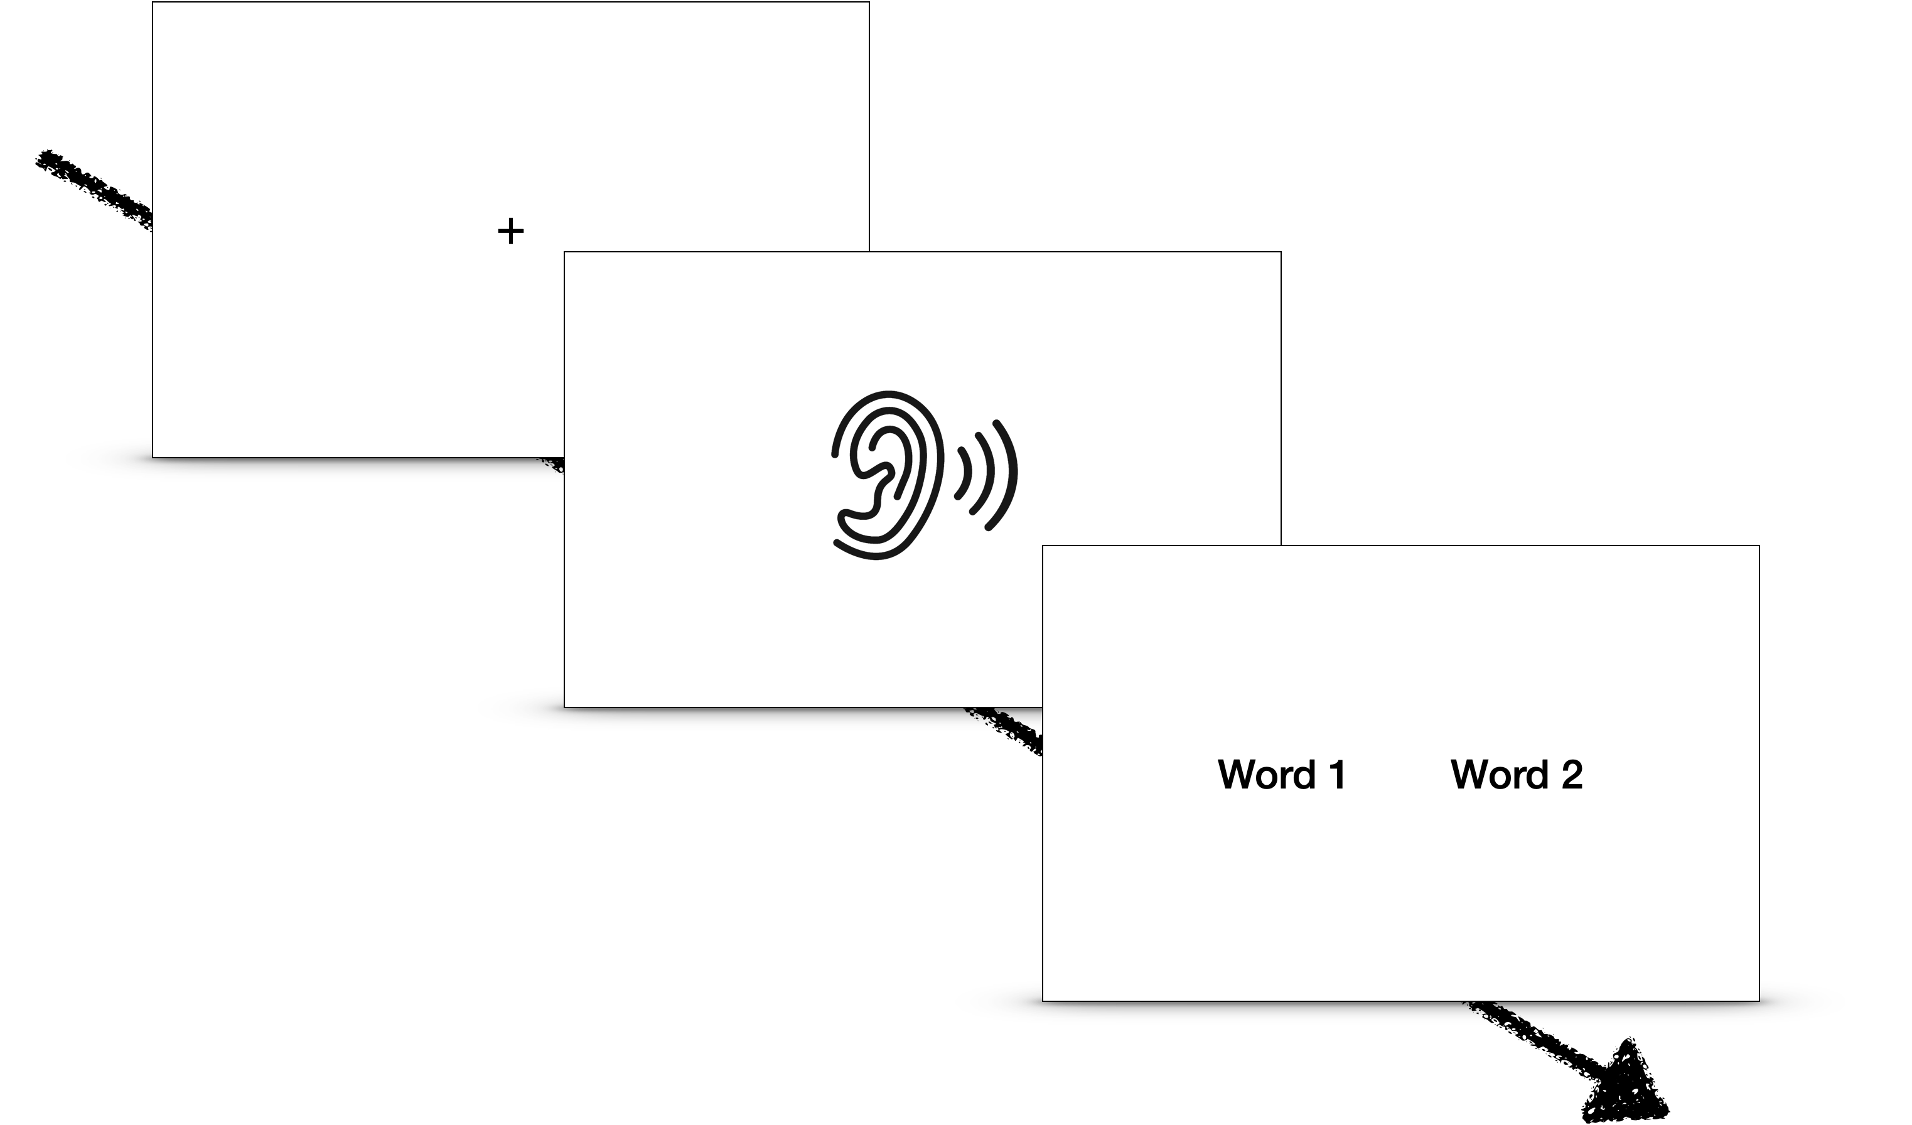
\includegraphics[scale=.25]{Figures/E2/Procedure.png}
\caption{Procedure of Experiment 2.}
\label{Figure:Experiment2Procedure}
\end{figure}

\subsection{Analyses}
The responses of the subjects were calculated as percentages of falling tone responses (cf. figure \ref{Figure:E2RawExample}), and then fitted through logistic regression models. A 25\% and a 75\% thresholds were set. Mean differences between the smallest and the largest crossing points on the two thresholds were taken as indicators of the magnitudes of perceptual compensation for tonal coarticulation. An illustration of such calculation is provided in figure \ref{Figure:E2ProcessedExample}.

\begin{figure}[h]
\centering
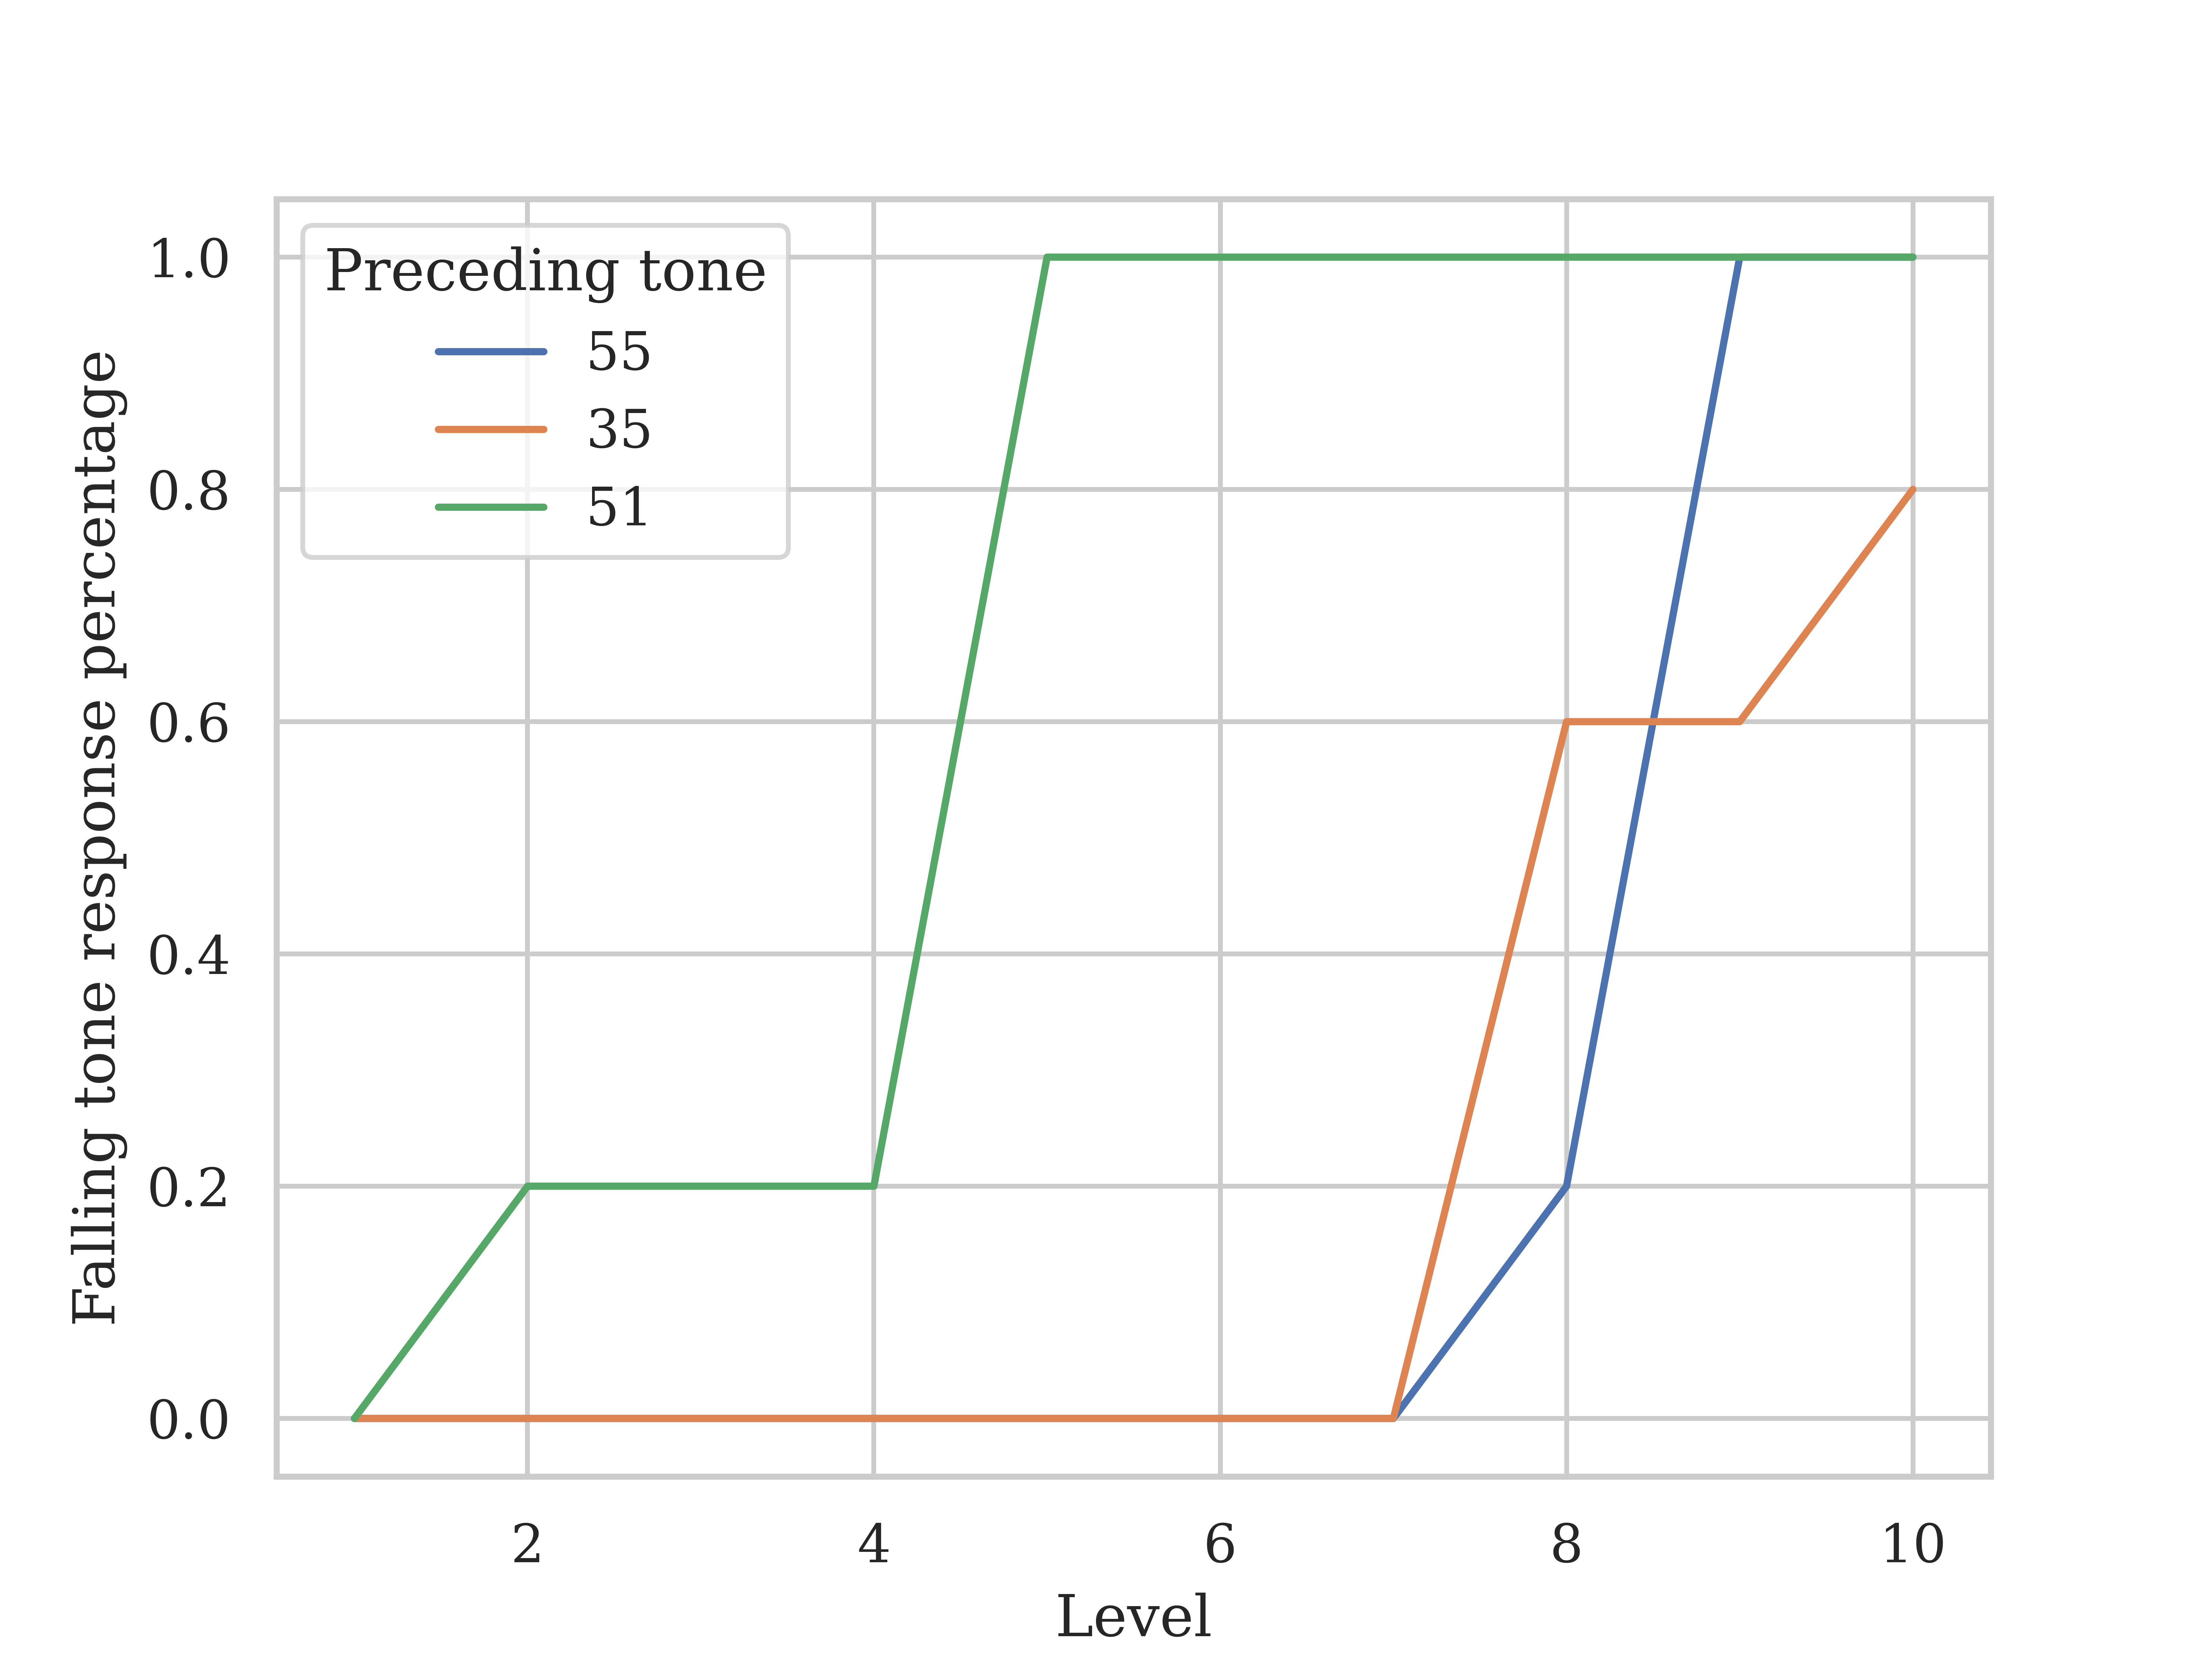
\includegraphics[scale=1]{Figures/E2/RawExample.png}
\caption{Example of percentages of falling tone responses (data of P1).}
\label{Figure:E2RawExample}
\end{figure}

\begin{figure}[h]
\centering
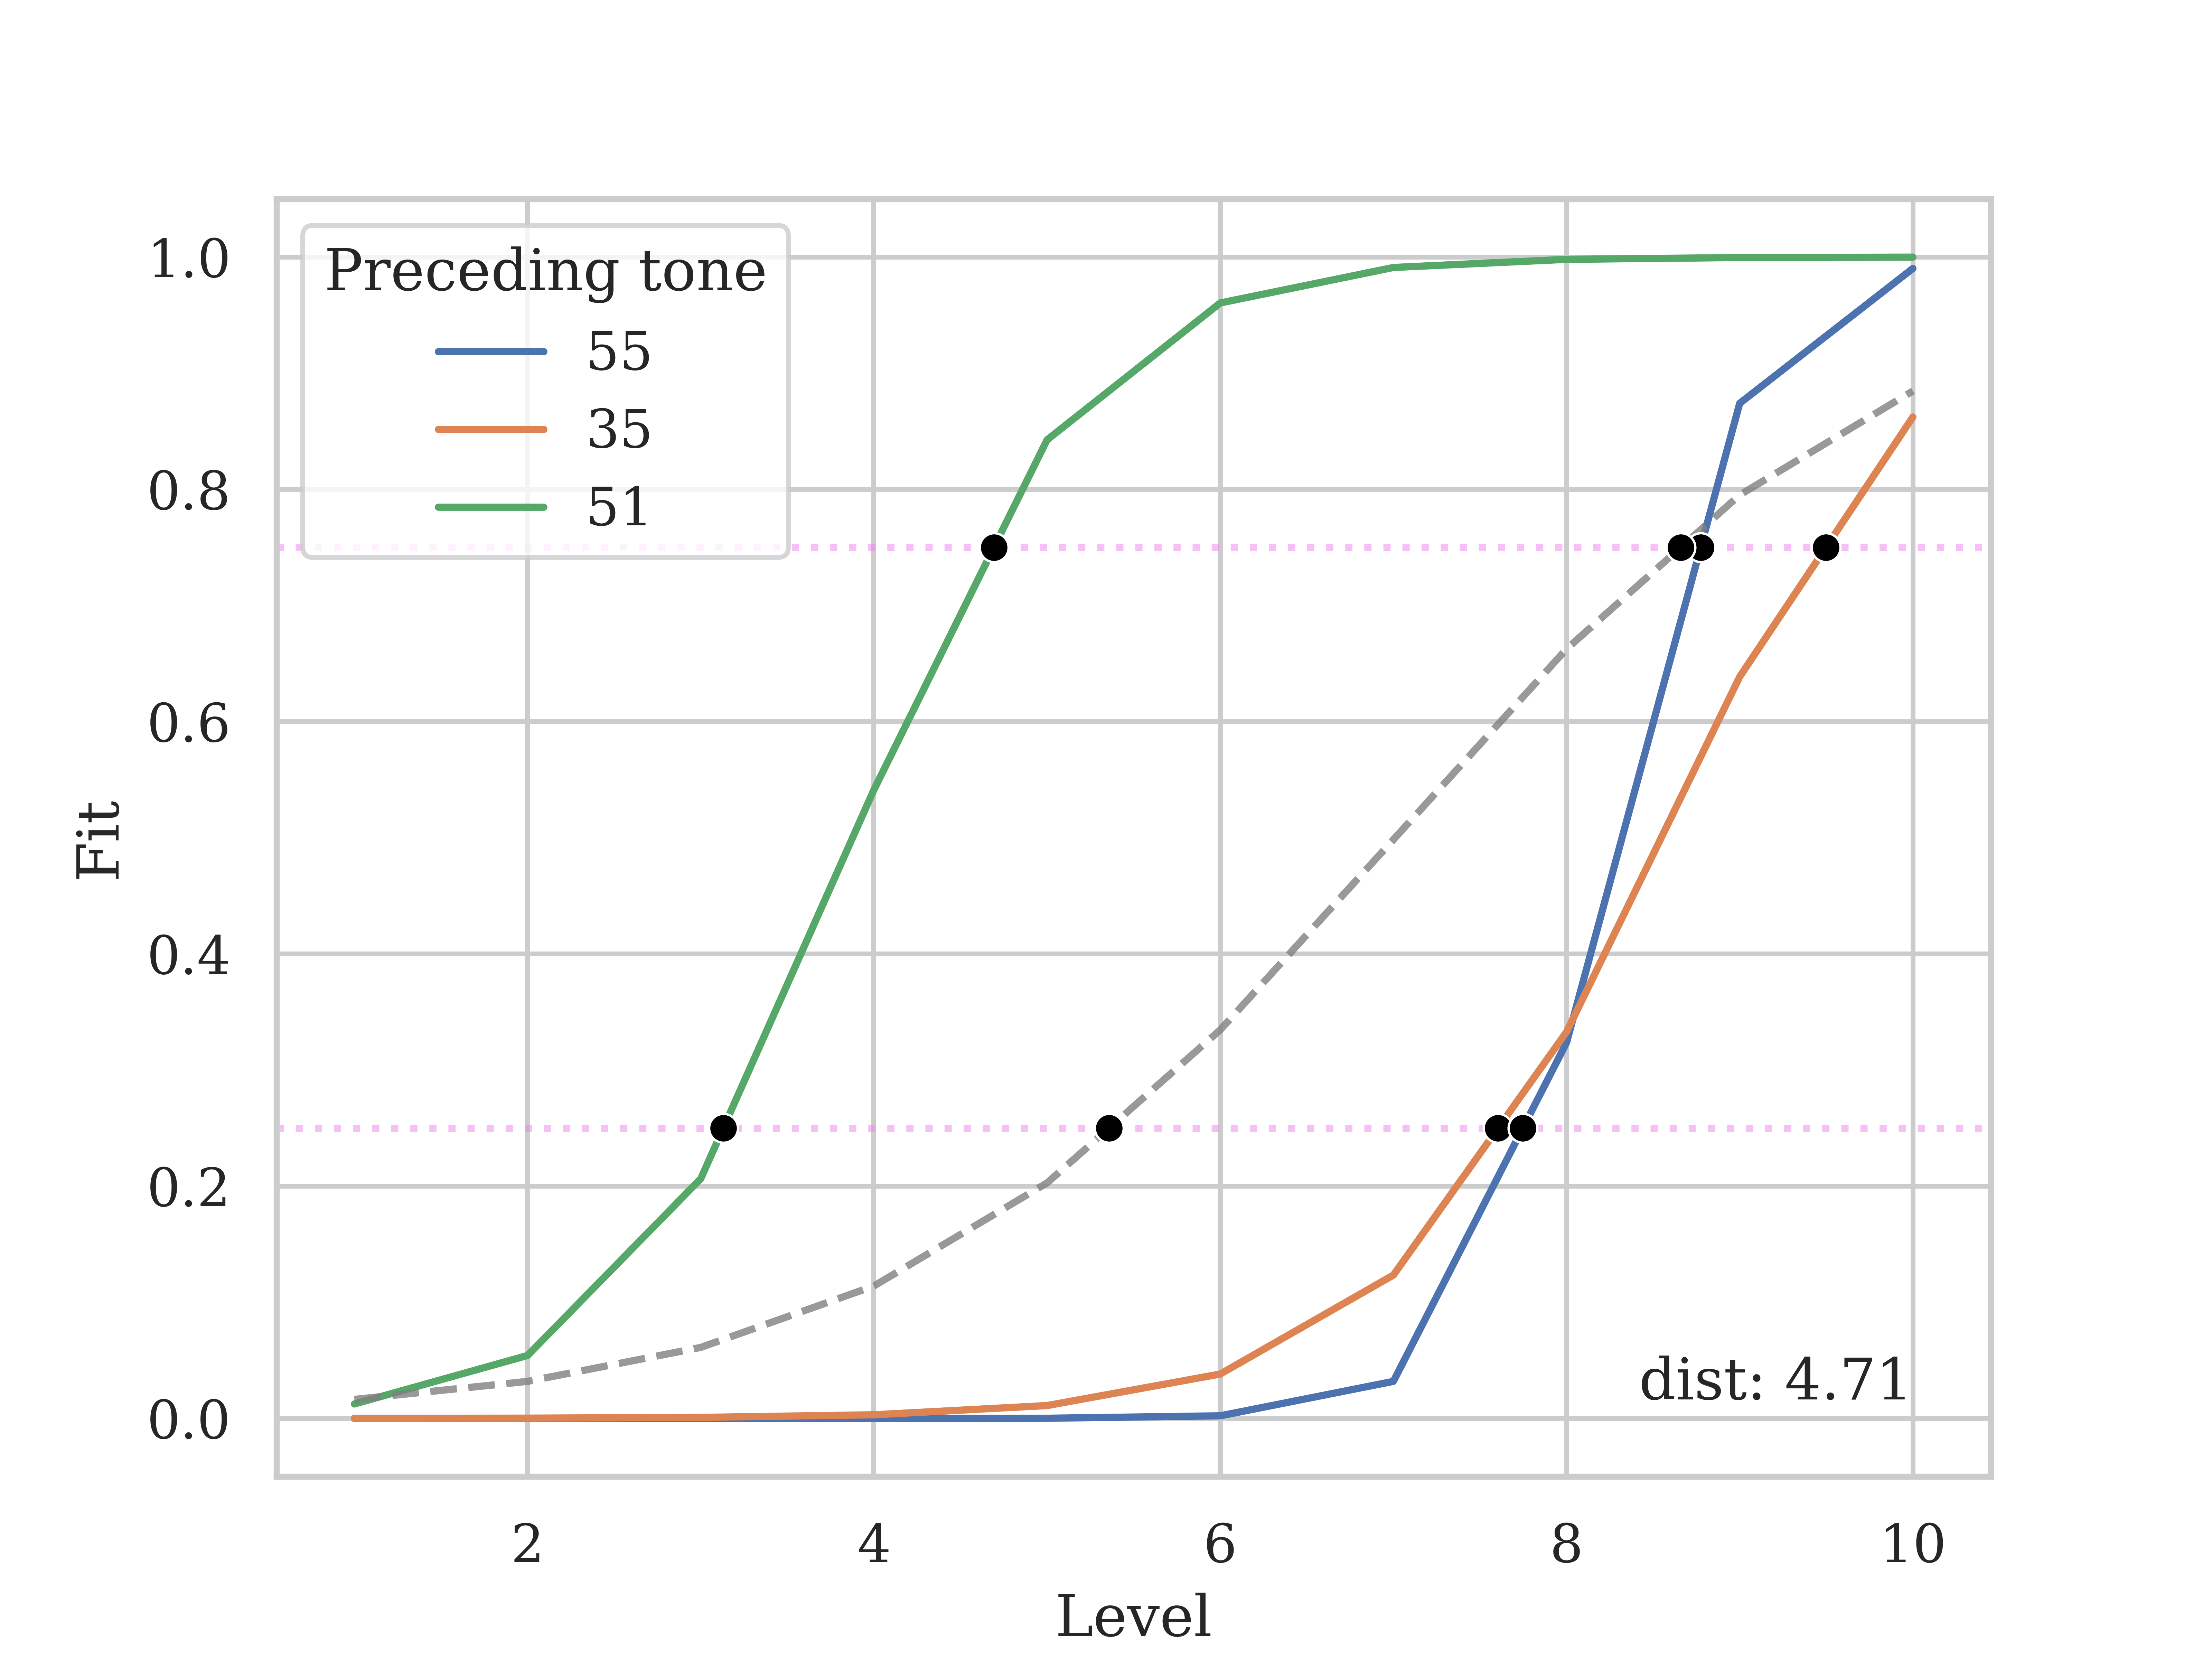
\includegraphics[scale=1]{Figures/E2/ProcessedExample.png}
\caption{Example of mean distance calculation (data of P1).}
\label{Figure:E2ProcessedExample}
\end{figure}

\section{Experiment 3}\label{section:Experiment3}
To explore the relation between perceptual compensation for tonal coarticulation and strictness of tone boundaries, Experiment 3 was conducted to see whether there exists differences between the acceptance ranges of falling and low-level tones in Taiwan Mandarin speakers and Taiwan Southern Min speakers.

To measure the subjects' strictness of tone boundaries, subjects listened to a continuum of falling and low-level tones after the high-level (55) tone (T1 in Taiwan Mandarin; T2' in Taiwan Southern Min), and were asked to judge whether what they heard were good tokens of the supposed target tones.

This experiment is also divided into the Mandarin and Southern Min versions.

\subsection{Participants}
The same subjects in Experiments 2 participated in this experiment. The monolingual group did the Mandarin version; the bilingual group did both the Mandarin and Southern Min versions.

\subsection{Stimuli}
\subsubsection{Word selection} In each version, 10 disyllabic words were used. All of their first syllables were the high-level tone. 5 of them had as their second syllables the falling tone, and 5 of them the low-level tone. There were therefore 2 groups of stimuli: 55 "(T1 in Taiwan Mandarin; T2' in Taiwan Southern Min)+51 (T4 in Taiwan Mandarin; T2 in Taiwan Southern Min) and 55+21 (T3 in Taiwan Mandarin and Taiwan Southern Min). The words were made sure to have no minimal pair counterparts; that is, the words in the 55+21 group would be non-words if the second syllables were changed into a falling tone, and vice versa. See Appendix \ref{Appendix:StimuliforExperiment3} for the words used.

\subsubsection{Stimuli recording and synthesis}
Stimuli were produced by the same speakers in Experiment 2, and recorded and synthesized the same way as in Experiment 2. Since the words, unlike those in Experiment 2, were not minimal pairs, a 55+21 stimulus would be less like a word as the level went up on the continuum, and vice versa for a 55+51 stimulus.

For each level of the 55+21 and 55+51 groups, there were 10 repetitions. For each repetition, one of the five words were randomly chosen. There were therefore a total of 200 (2 groups$\times$10 levels$\times$10 repetitions) stimuli.

\subsection{Procedure}
This experiment was conducted after Experiment 2, after a minimal 1 minute break. The procedure and presentation were the same as those of Experiment 2, except that only one word was presented in the middle of the screen, with two buttons, a cross and a circle, underneath. The subject was asked to decide whether he/she thought it was a correct production of the word they saw. Figure \ref{Figure:Experiment3Procedure} illustrates such process. Participants were familiarized with the stimuli the same way as in Experiment 2.

\begin{figure}[h]
\centering
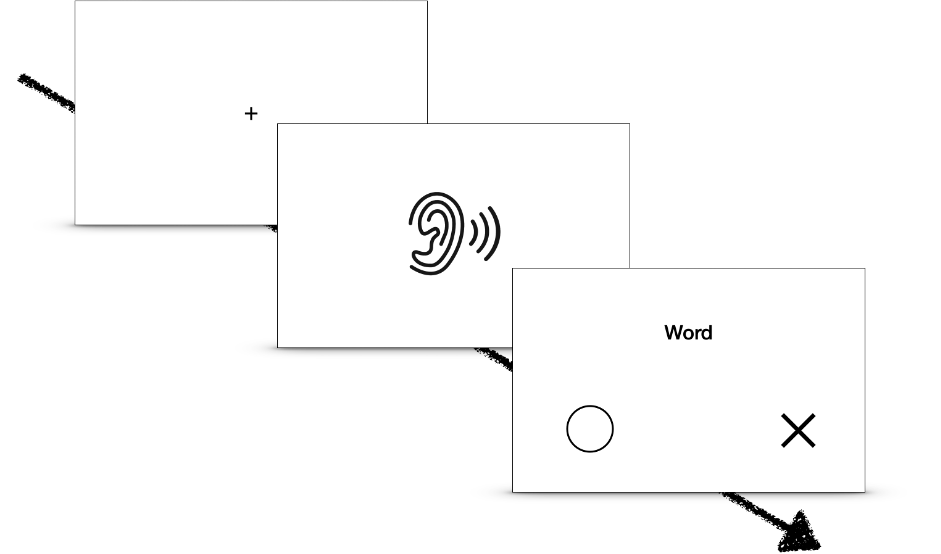
\includegraphics[scale=1]{Figures/E3/Procedure.png}
\caption{Procedure of Experiment 3.}
\label{Figure:Experiment3Procedure}
\end{figure}

\subsection{Analyses}
The subjects' responses were calculated as percentages and taken as acceptance rates of each of the 10 levels. These were then fitted through logistic regression models. The maximum slopes of each regression lines were taken as indicators of how strict/tolerant the subjects' tonal acceptances were. A steep slope would indicate that the subject was very strict on how the pitch values/contours of a given tone should be, and a flatter slope would suggest the subject had a wider acceptance range for the pitch of a given tone. An illustration is provided in figure \ref{Figure:E3ProcessedExample}.

\begin{figure}[h]
\centering
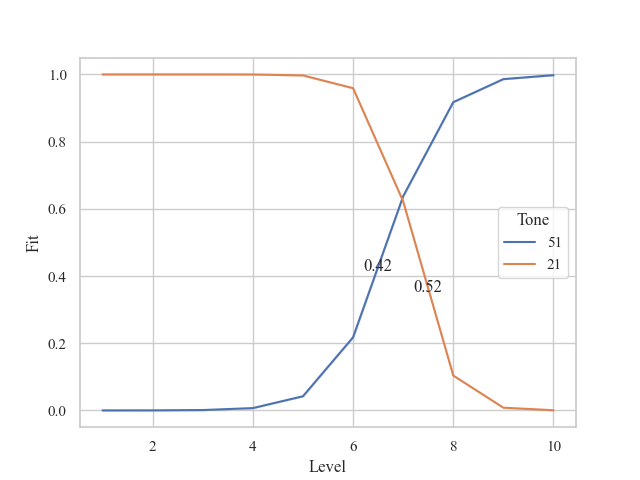
\includegraphics[scale=1]{Figures/E3/ProcessedExample.png}
\caption{Example of maximum slope calculation (data of P1).}
\label{Figure:E3ProcessedExample}
\end{figure}

%===Results===
\pagebreak
\chapter{Results}
\section{Taiwan Mandarin and Taiwan Southern Min tones under coarticulation}

\subsection{Tone contours}

Tone contours of Taiwan Mandarin and Taiwan Southern Min tones in carryover and anticipatory positions are shown in Appendix \ref{Appendix:ToneContours}.

\subsection{Directionalities and magnitudes of coarticulatory effects in the two languages}

Tonal coarticulation of Taiwan Mandarin and Taiwan Southern Min in carry-over and anticipatory positions respectively are shown in figures \ref{Figure:LMMCarryover} and \ref{Figure:LMMAnticipatory}. Rather similar distributions of coarticulatory effects were found for both languages. For both languages, in both positions, the ambient tones were shown to exert positive impact on the target tones, that is, a high ambient tone raised, and a low ambient tone lowered the target tone. In terms of magnitudes, for both positions, no significant difference was found between the two languages. Meaning the two languages showed a similar degree of carry-over and anticipatory effects. Within-language comparisons also revealed essentially no difference between the two kinds of effects in both Taiwan Mandarin and Taiwan Southern Min.

\begin{figure}[hbt!]
\centering
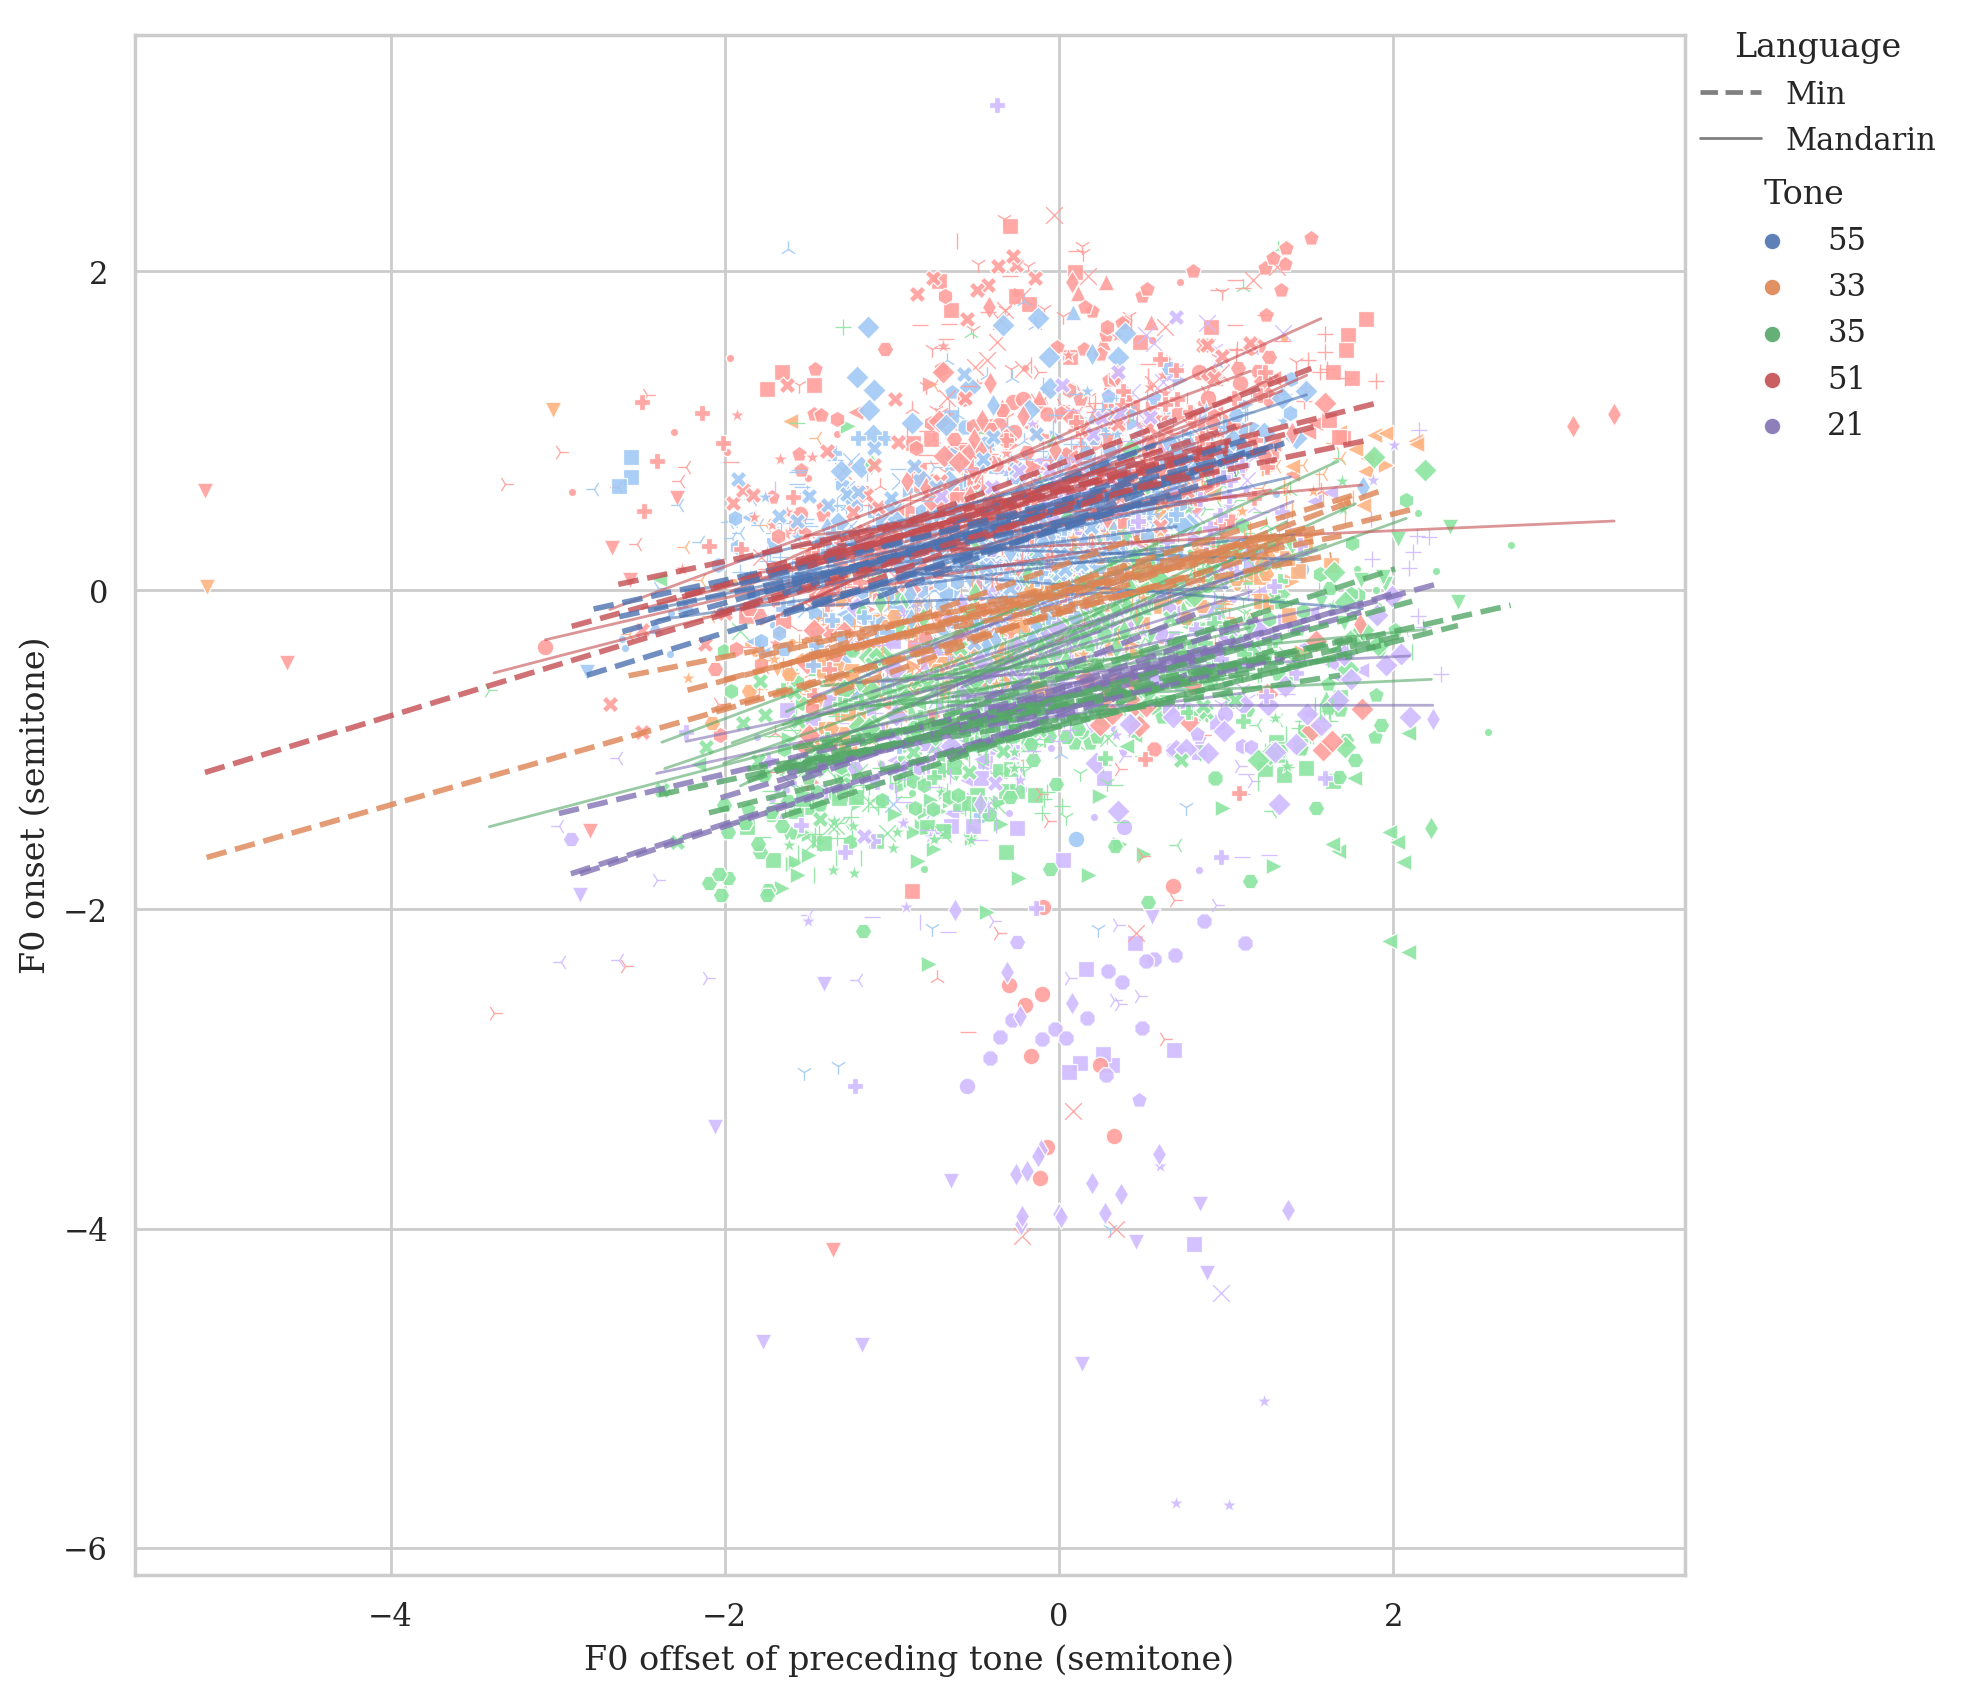
\includegraphics[scale=.45, trim={0 .5cm 0 0}]{Figures/E1/Carryover.png}
\caption{Fitted LMM model of tone onsets and offsets in carry-over positions.}
\label{Figure:LMMCarryover}
\end{figure}

\begin{figure}[hbt!]
\centering
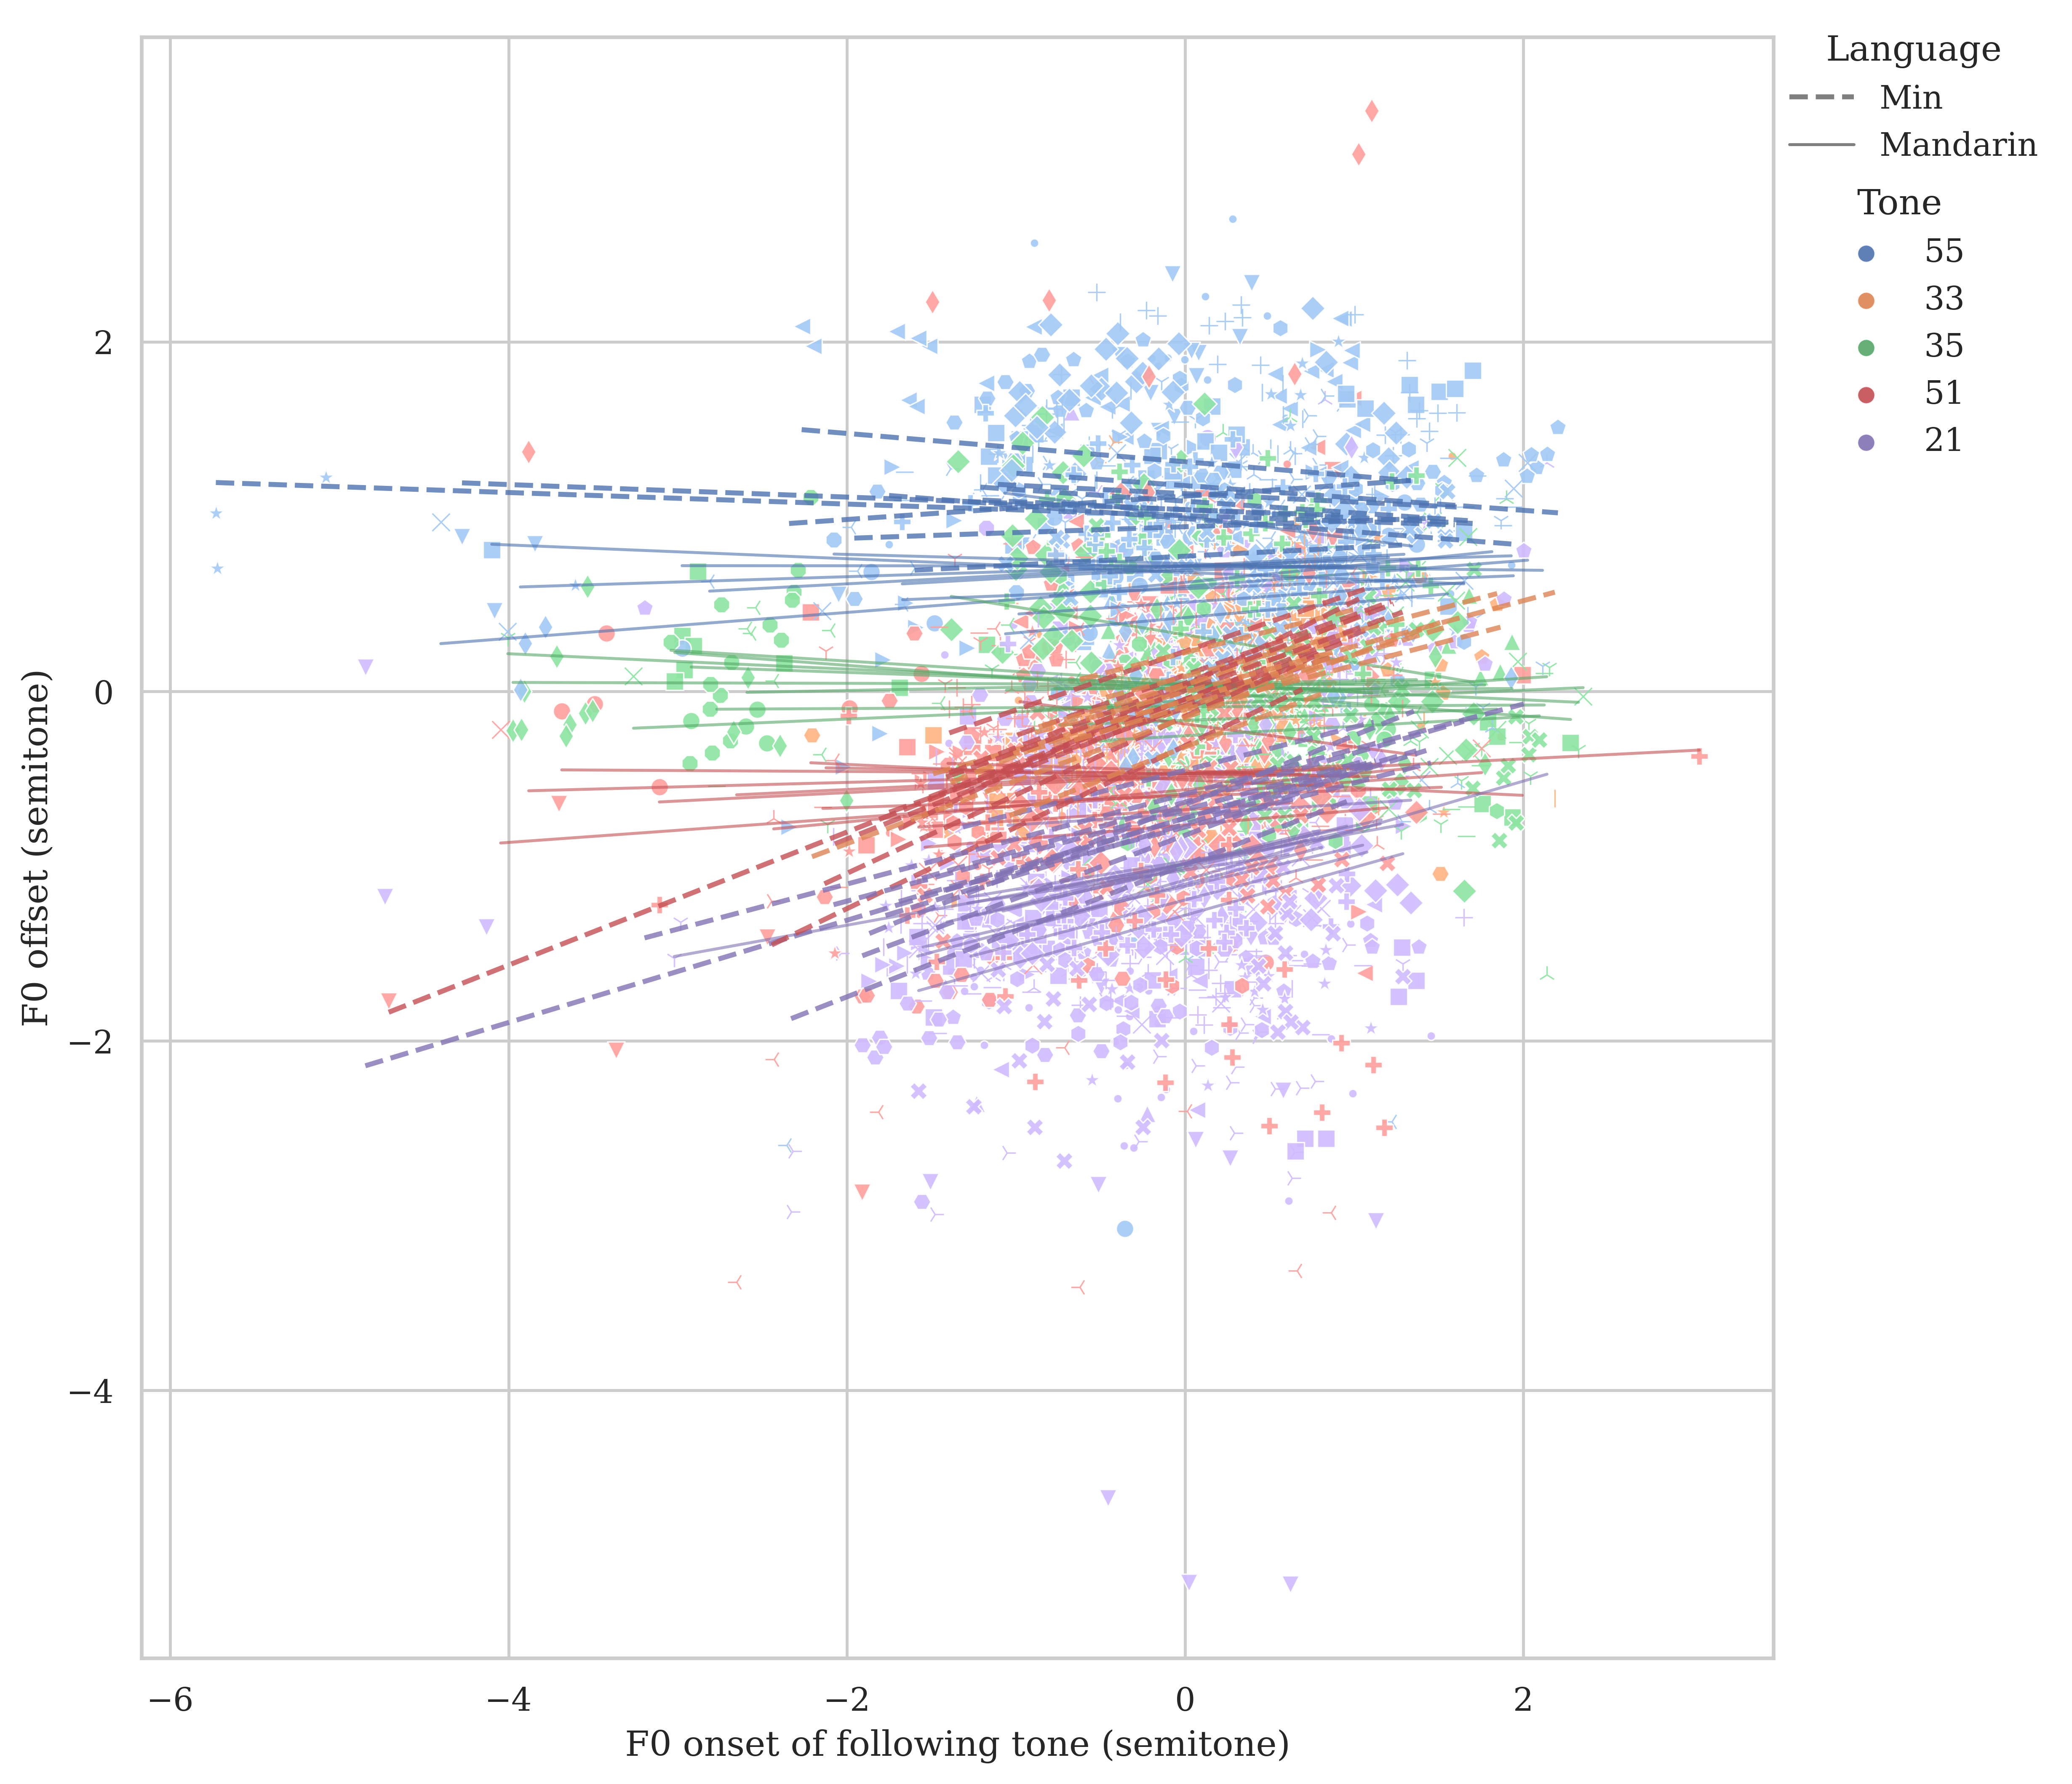
\includegraphics[scale=.45, trim={0 .5cm 0 0}]{Figures/E1/Anticipatory.png}
\caption{Fitted LMM model of tone onsets and offsets in anticipatory positions.}
\label{Figure:LMMAnticipatory}
\end{figure}

In general, tonal coarticulation in Taiwan Mandarin and Taiwan Southern Min were almost identical in both directionality and magnitudes. Symmetries were found in both languages, and no difference of magnitude was found. This can be summarized in tables \ref{table:MandarinMinDistribution} and \ref{table:MandarinMinDistributionComparison}.

\begin{flushleft}
\begin{table}[hbt!]
\begin{tabularx}{\textwidth}{l|X|X|}
\cline{2-3}
 & Magnitude & Direction \\
%\hhline{-::==}
\hhline{~|--}\noalign{\vspace*{\doublerulesep}}
\hhline{-||--}
\multicolumn{1}{|X||}{Carry-over} & \multirow{2}{*}{Equally strong} & \multirow{2}{*}{Assimilatory}\\
\hhline{|-||~~}
\multicolumn{1}{|X||}{Anticipatory} &  & \\
\hhline{|-||-|-|}
\end{tabularx}
\caption{Distribution of tonal coarticulation in Taiwan Mandarin and Taiwan Southern Min}
\label{table:MandarinMinDistribution}
\end{table}
\end{flushleft}

\begin{flushleft}
\begin{table}[hbt!]
\begin{tabularx}{\textwidth}{l|X|X|}
\cline{2-3}
 & Carry-over & Anticipatory \\
\hhline{~|--}\noalign{\vspace*{\doublerulesep}}
\hhline{-||--}
\multicolumn{1}{|X||}{Taiwan Mandarin} & \multirow{2}{*}{Equally strong} & \multirow{2}{*}{Equally strong}\\
\hhline{|-||~~}
\multicolumn{1}{|X||}{Taiwan Southern Min} &  & \\
\hhline{|-||-|-|}
\end{tabularx}
\caption{Comparison of tonal coarticulation between Taiwan Mandarin and Taiwan Southern Min}
\label{table:MandarinMinDistributionComparison}
\end{table}
\end{flushleft}

\section{Normalization for tonal coarticulation in Taiwan Mandarin and Taiwan Southern Min}
Fitted falling tone responses of the the monolingual and bilingual groups in Mandarin and Southern Min are shown in Figure \ref{Figure:E2Raw}.

\begin{figure}[hbt!]
\centering
\begin{subfigure}[b]{.45\textwidth}
\centering
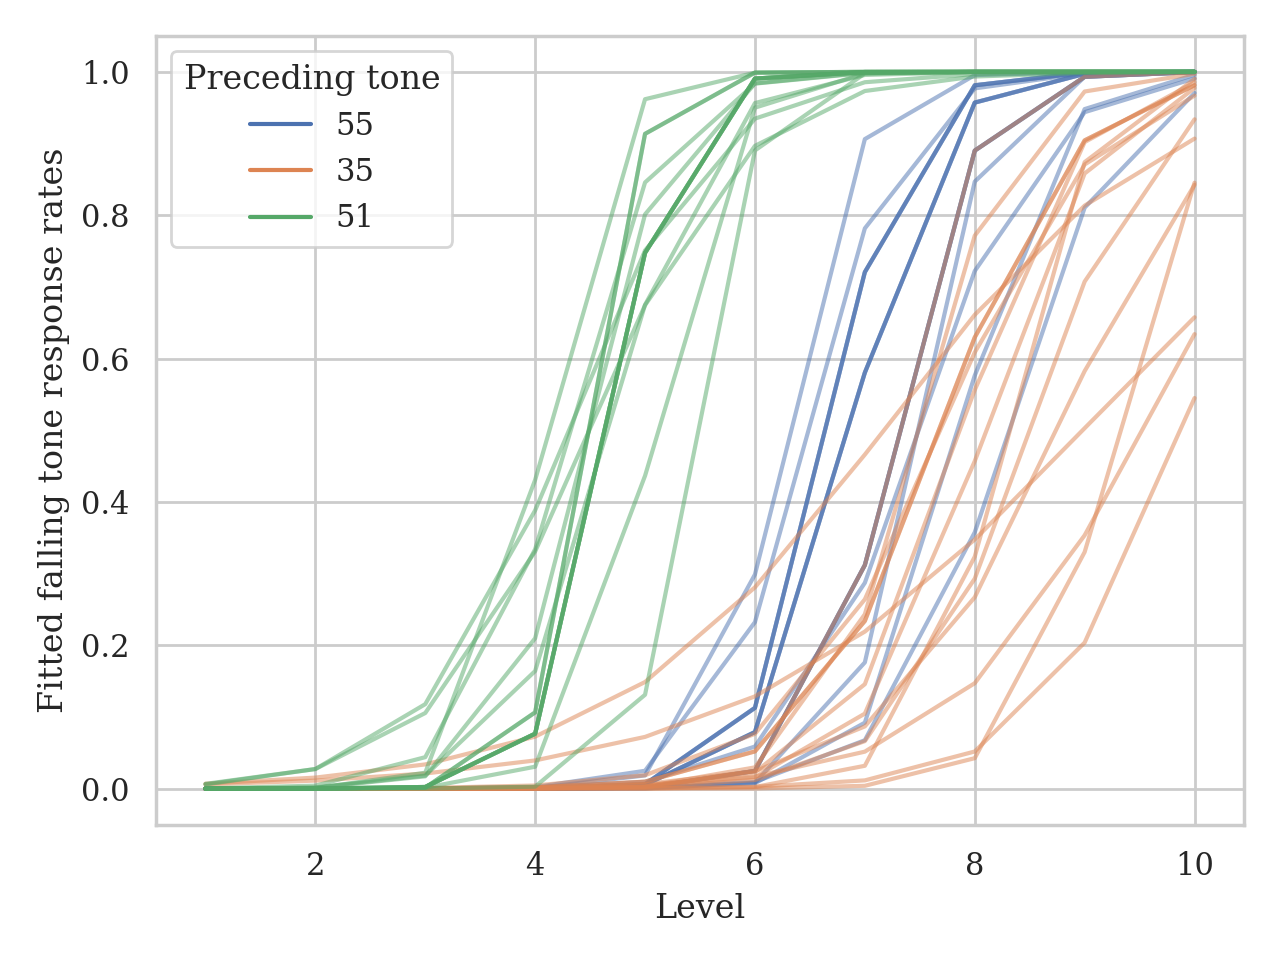
\includegraphics[width=\textwidth]{Figures/E2/Mandarin_monolingual_E2_raw.png}
\end{subfigure}
\hfill
\begin{subfigure}[b]{.45\textwidth}
\centering
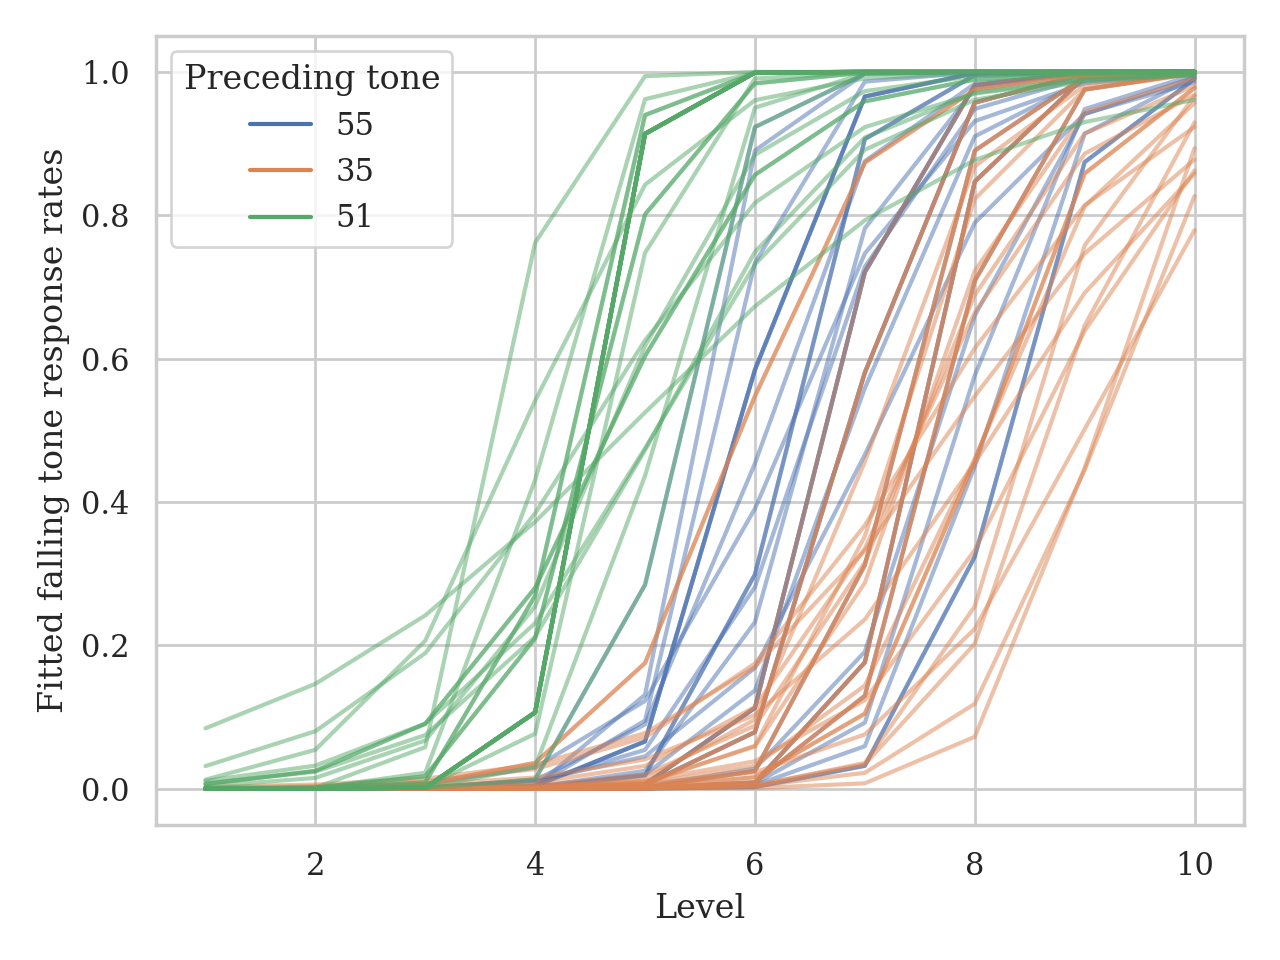
\includegraphics[width=\textwidth]{Figures/E2/Mandarin_bilingual_E2_raw.png}
\end{subfigure}
\hfill
\begin{subfigure}[b]{.45\textwidth}
\centering
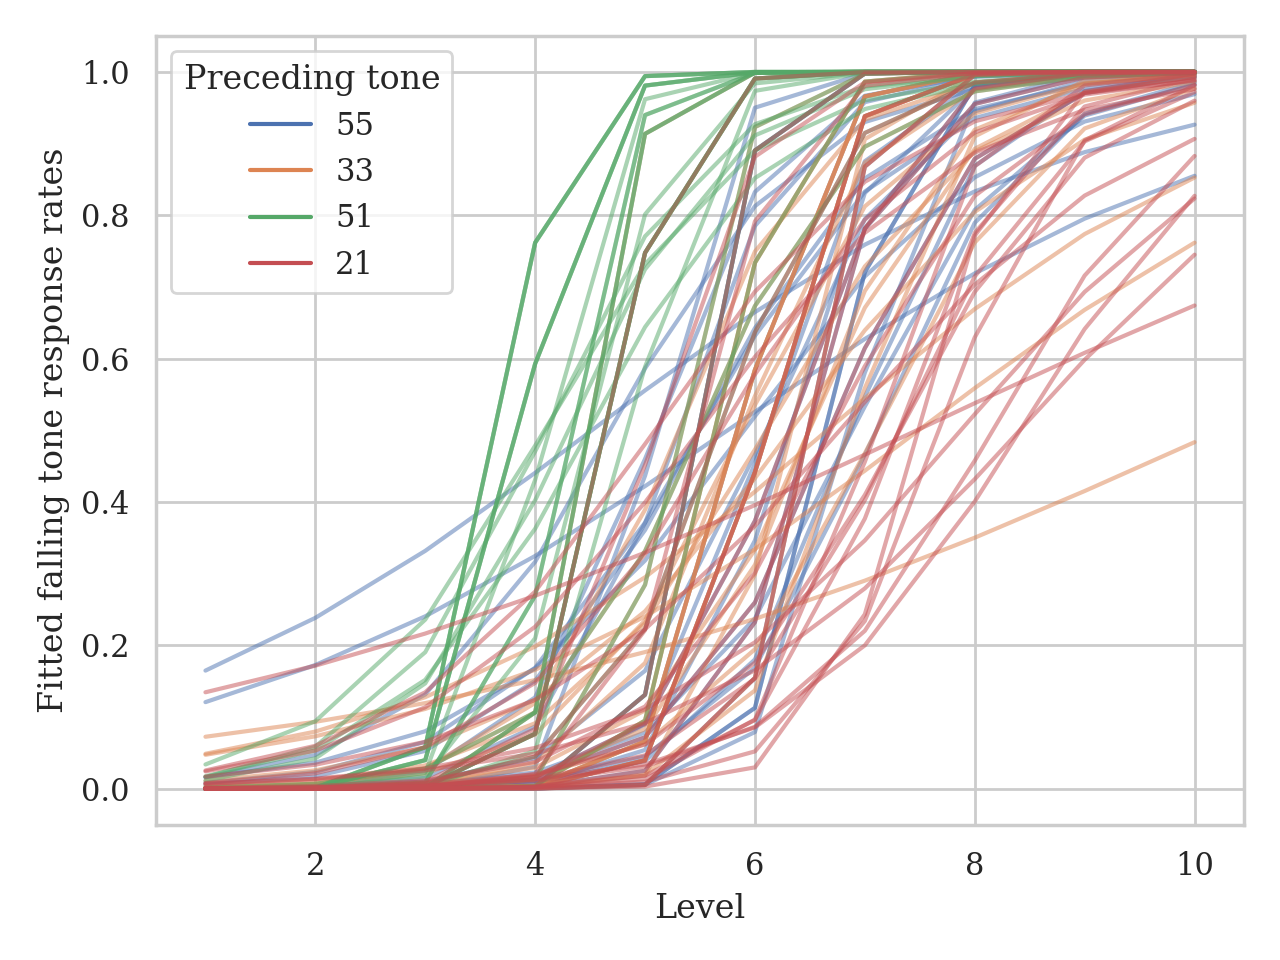
\includegraphics[width=\textwidth]{Figures/E2/Min_E2_raw.png}
\end{subfigure}
\caption{Falling tone response percentages in Experiment 2 (top left: Mandarin (monolingual); top right: Mandarin (bilingual); bottom: Southern Min).}
\label{Figure:E2Raw}
\end{figure}

Upon first sight, we see an obvious difference between the monolingual group's Mandarin results and the bilingual group's Southern Min results, with the latter being generally narrower. The means of the maximum distances between these low-tone-to-falling-tone responses on the 0.25 and 0.75 thresholds are shown in figure \ref{Figure:DistBoxPlot}.

\begin{figure}[hbt!]
\centering
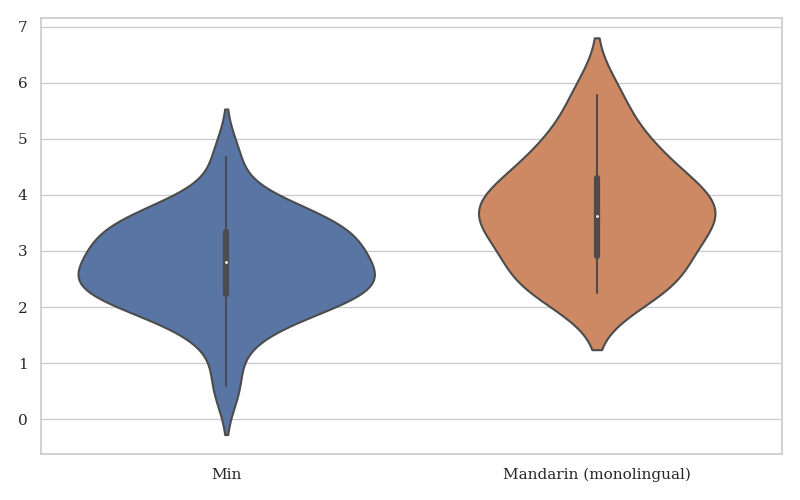
\includegraphics[scale=.7, trim={0 .5cm 0 0}]{Figures/E2/Result.png}
\caption{Calculated mean maximum distances (level) in Experiment 2.}
\label{Figure:DistBoxPlot}
\end{figure}

%A one-way ANOVA revealed that there was significant difference between at least two of the Southern Min results, and the monolingual and bilingual groups' Mandarin results (F(2, 62)=5.53, p<.01**).

As mentioned in section \ref{section:Experiment2}, this measurement serves as a means of quantification of the magnitudes of perceptual normalization for tonal coarticulation. A simple t-test showed that the the distances in Taiwan Southern Min are significantly shorter than the distances in Mandarin on the monolingual group (p<.001**)\footnote{Post-hoc power analyses have been done for this and following reported significant results, all results gained a power of 71\% or higher.}. This suggests that normalization for tonal coarticulation was of a smaller amplitude in Taiwan Southern Min than in Taiwan Mandarin. Interestingly, this difference between Mandarin and Southern Min was present not only between groups, but also within subjects, as shown in figure \ref{Figure:DistBilingualBoxPlot}. A paired t-test showed that even on the same speakers of the advanced bilingual group, this normalization was stronger in Mandarin than in Southern Min (p<.05*). This linguistic discrepancy, however, faded away on intermediate bilinguals (p=.32).

\begin{figure}[hbt!]
\centering
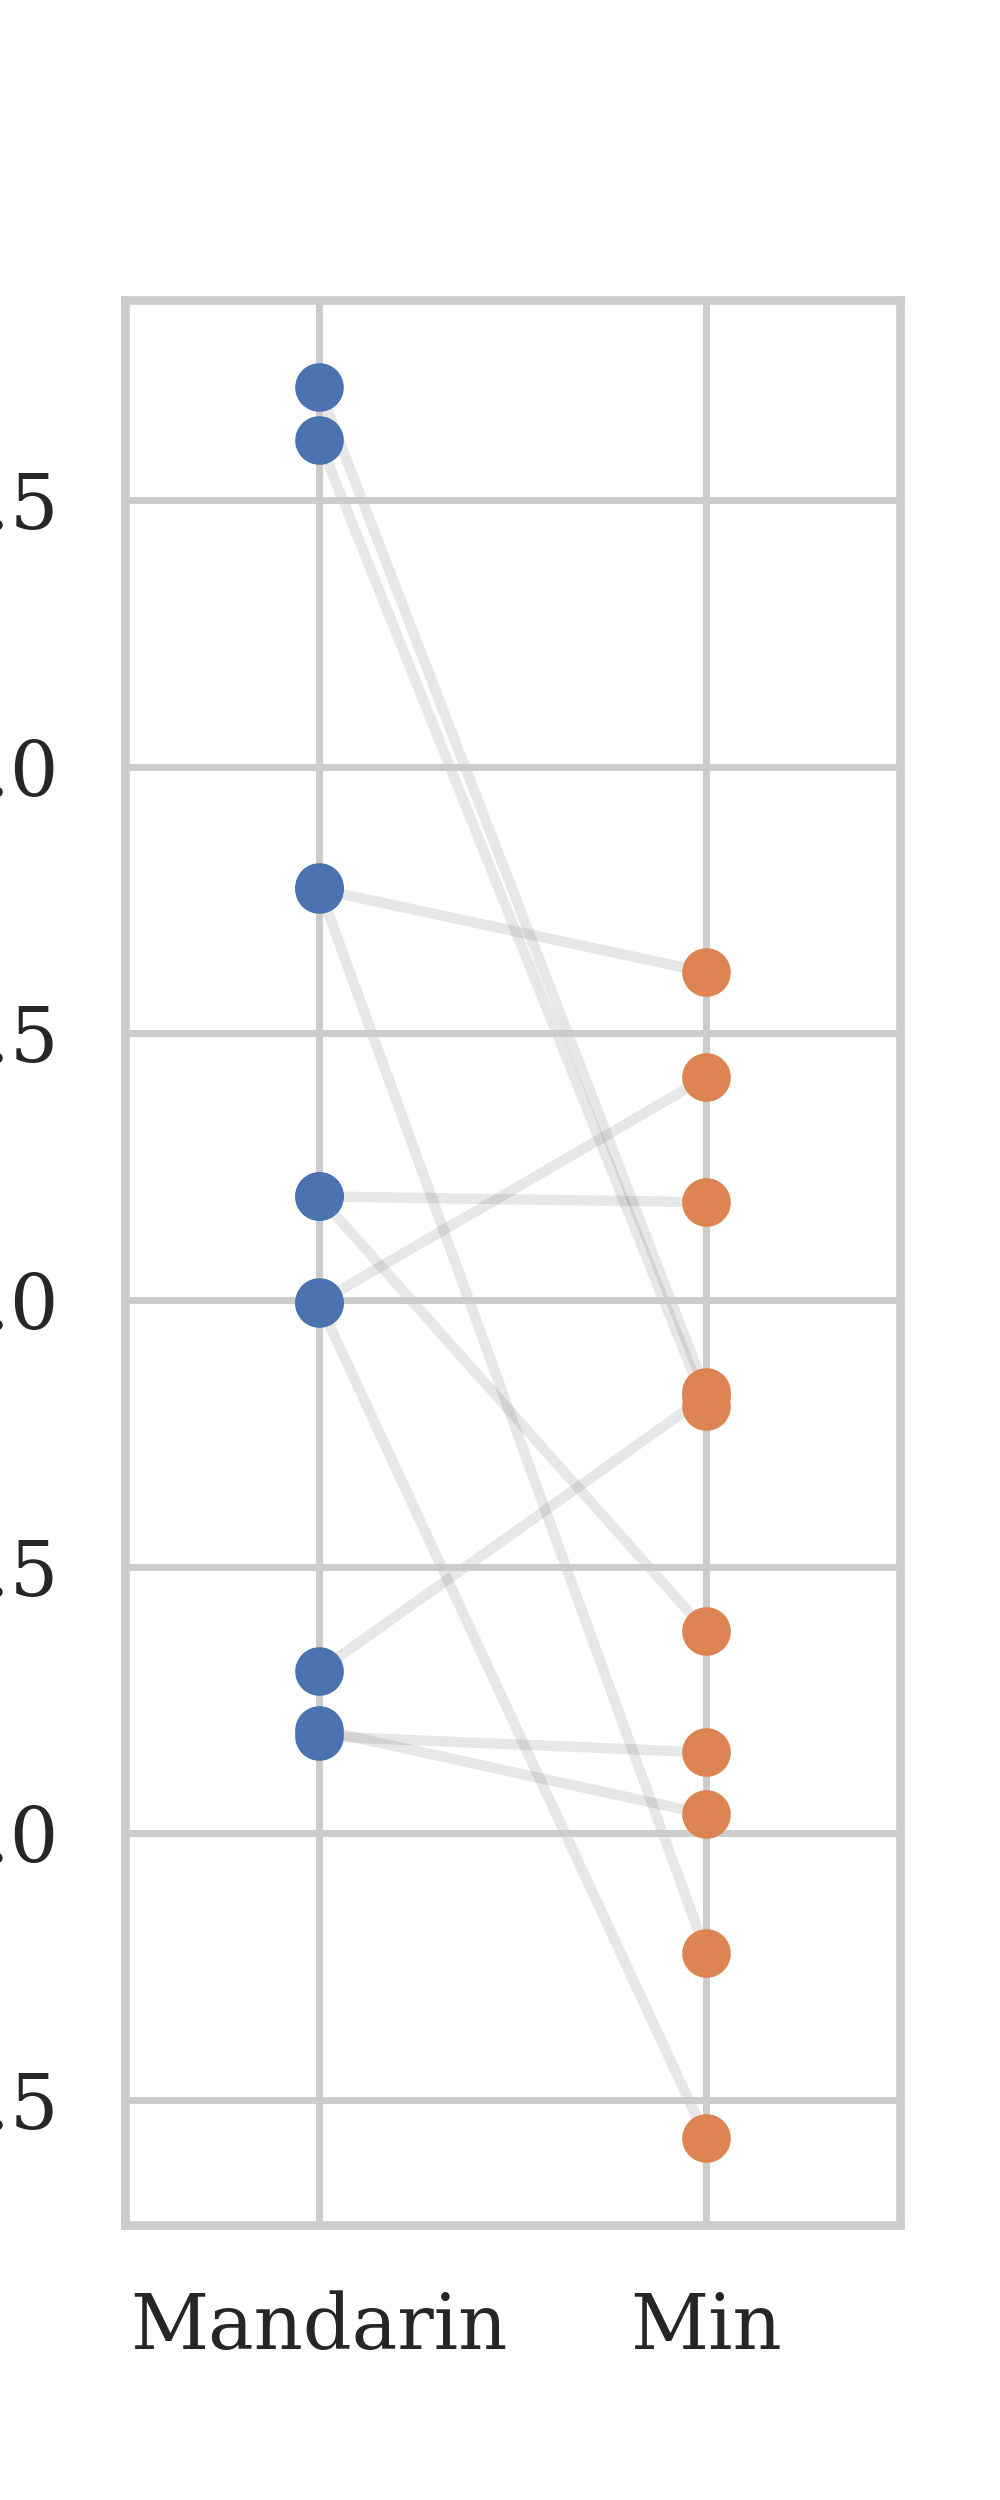
\includegraphics[scale=1, trim={0 .5cm 0 0}]{Figures/E2/Result_bilingual.png}
\caption{Pairwise comparison of calculated mean maximum distances (level) of advanced bilingual subjects in Experiment 2.}
\label{Figure:DistBilingualBoxPlot}
\end{figure}

\section{Tone boundaries between the low tone and the falling tone in Mandarin and Taiwan Southern Min}

Fitted acceptance rates of the falling tone and the low tone in Mandarin and Southern Min of the monolingual and bilingual groups are shown in Figure \ref{Figure:E3Raw}.

\begin{figure}[hbt!]
\centering
\begin{subfigure}[b]{.45\textwidth}
\centering
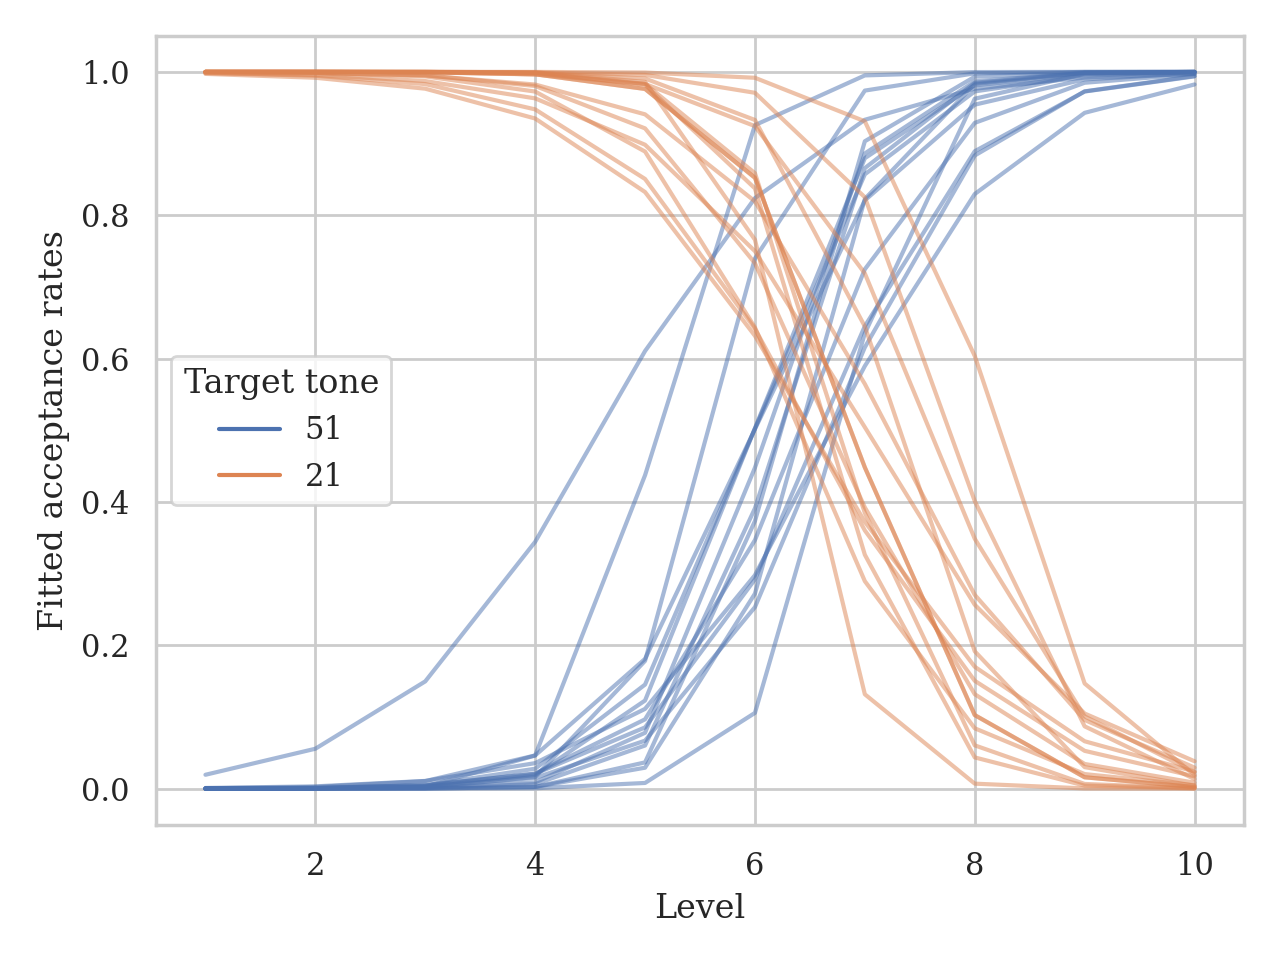
\includegraphics[width=\textwidth]{Figures/E3/Mandarin_monolingual_E3_raw.png}
\end{subfigure}
\hfill
\begin{subfigure}[b]{.45\textwidth}
\centering
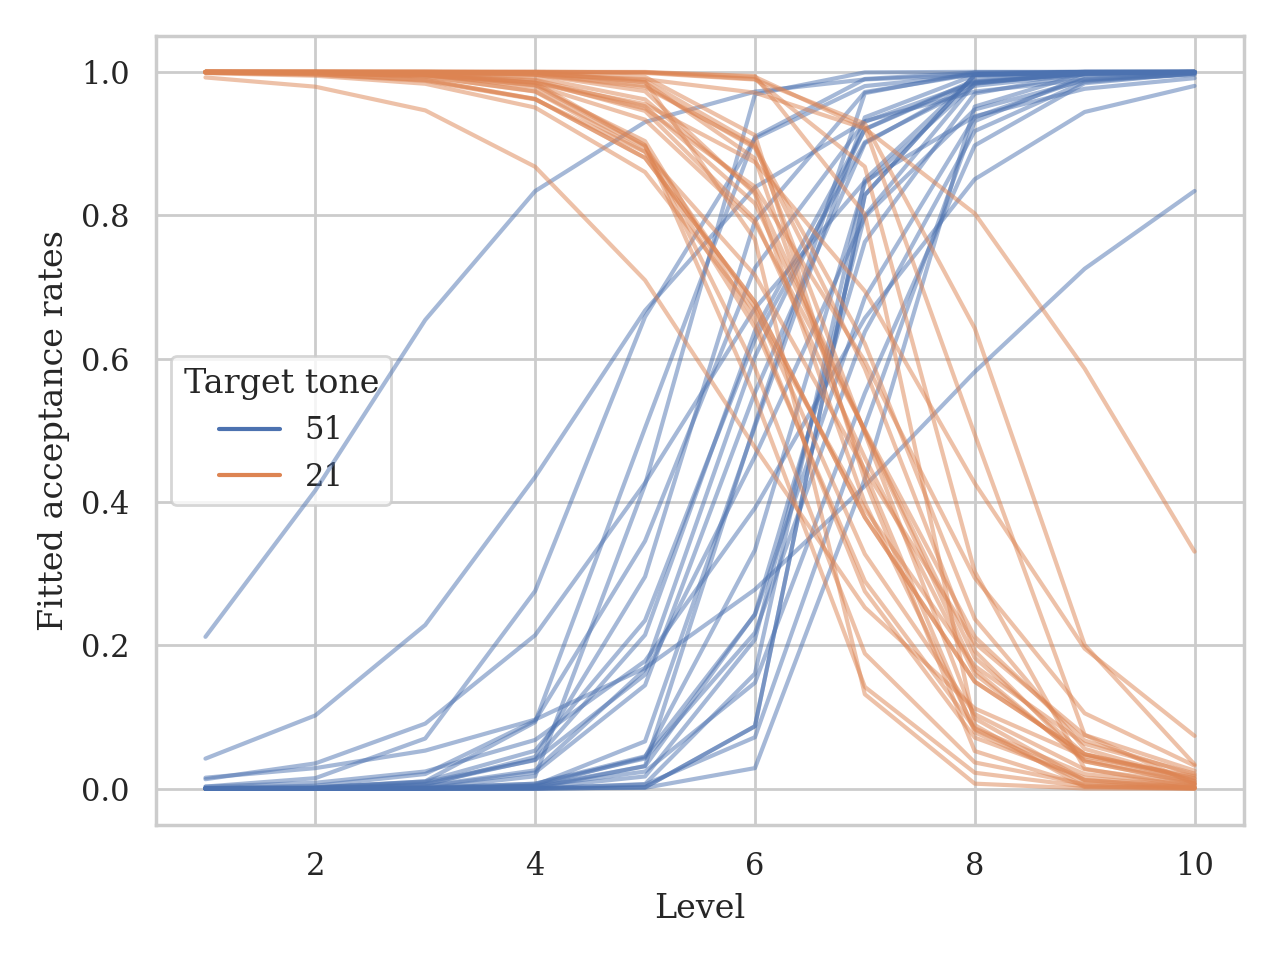
\includegraphics[width=\textwidth]{Figures/E3/Mandarin_bilingual_E3_raw.png}
\end{subfigure}
\hfill
\begin{subfigure}[b]{.45\textwidth}
\centering
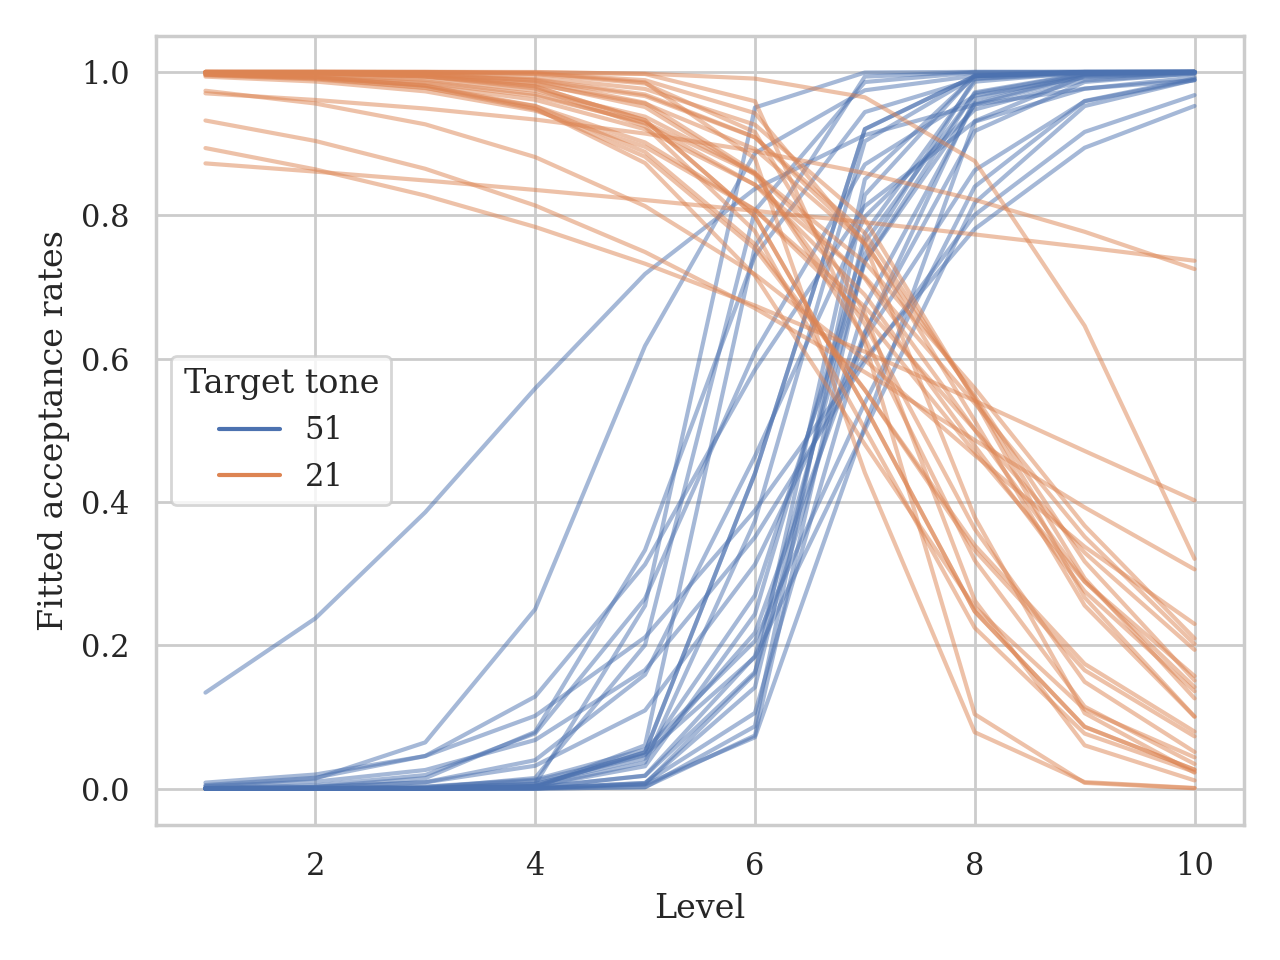
\includegraphics[width=\textwidth]{Figures/E3/Min_E3_raw.png}
\end{subfigure}
\caption{Acceptance rates in Experiment 3 (top left: Mandarin (monolingual); top right: Mandarin (bilingual); bottom: Southern Min).}
\label{Figure:E3Raw}
\end{figure}

In general, we see that the falling tone had stricter boundaries than the low tone. Maximum slopes of the regressions of the two tones in Mandarin and Southern Min are shown in Figure \ref{Figure:E3BoxPlot}.

\begin{figure}[hbt!]
\centering
\begin{subfigure}[b]{.49\textwidth}
\centering
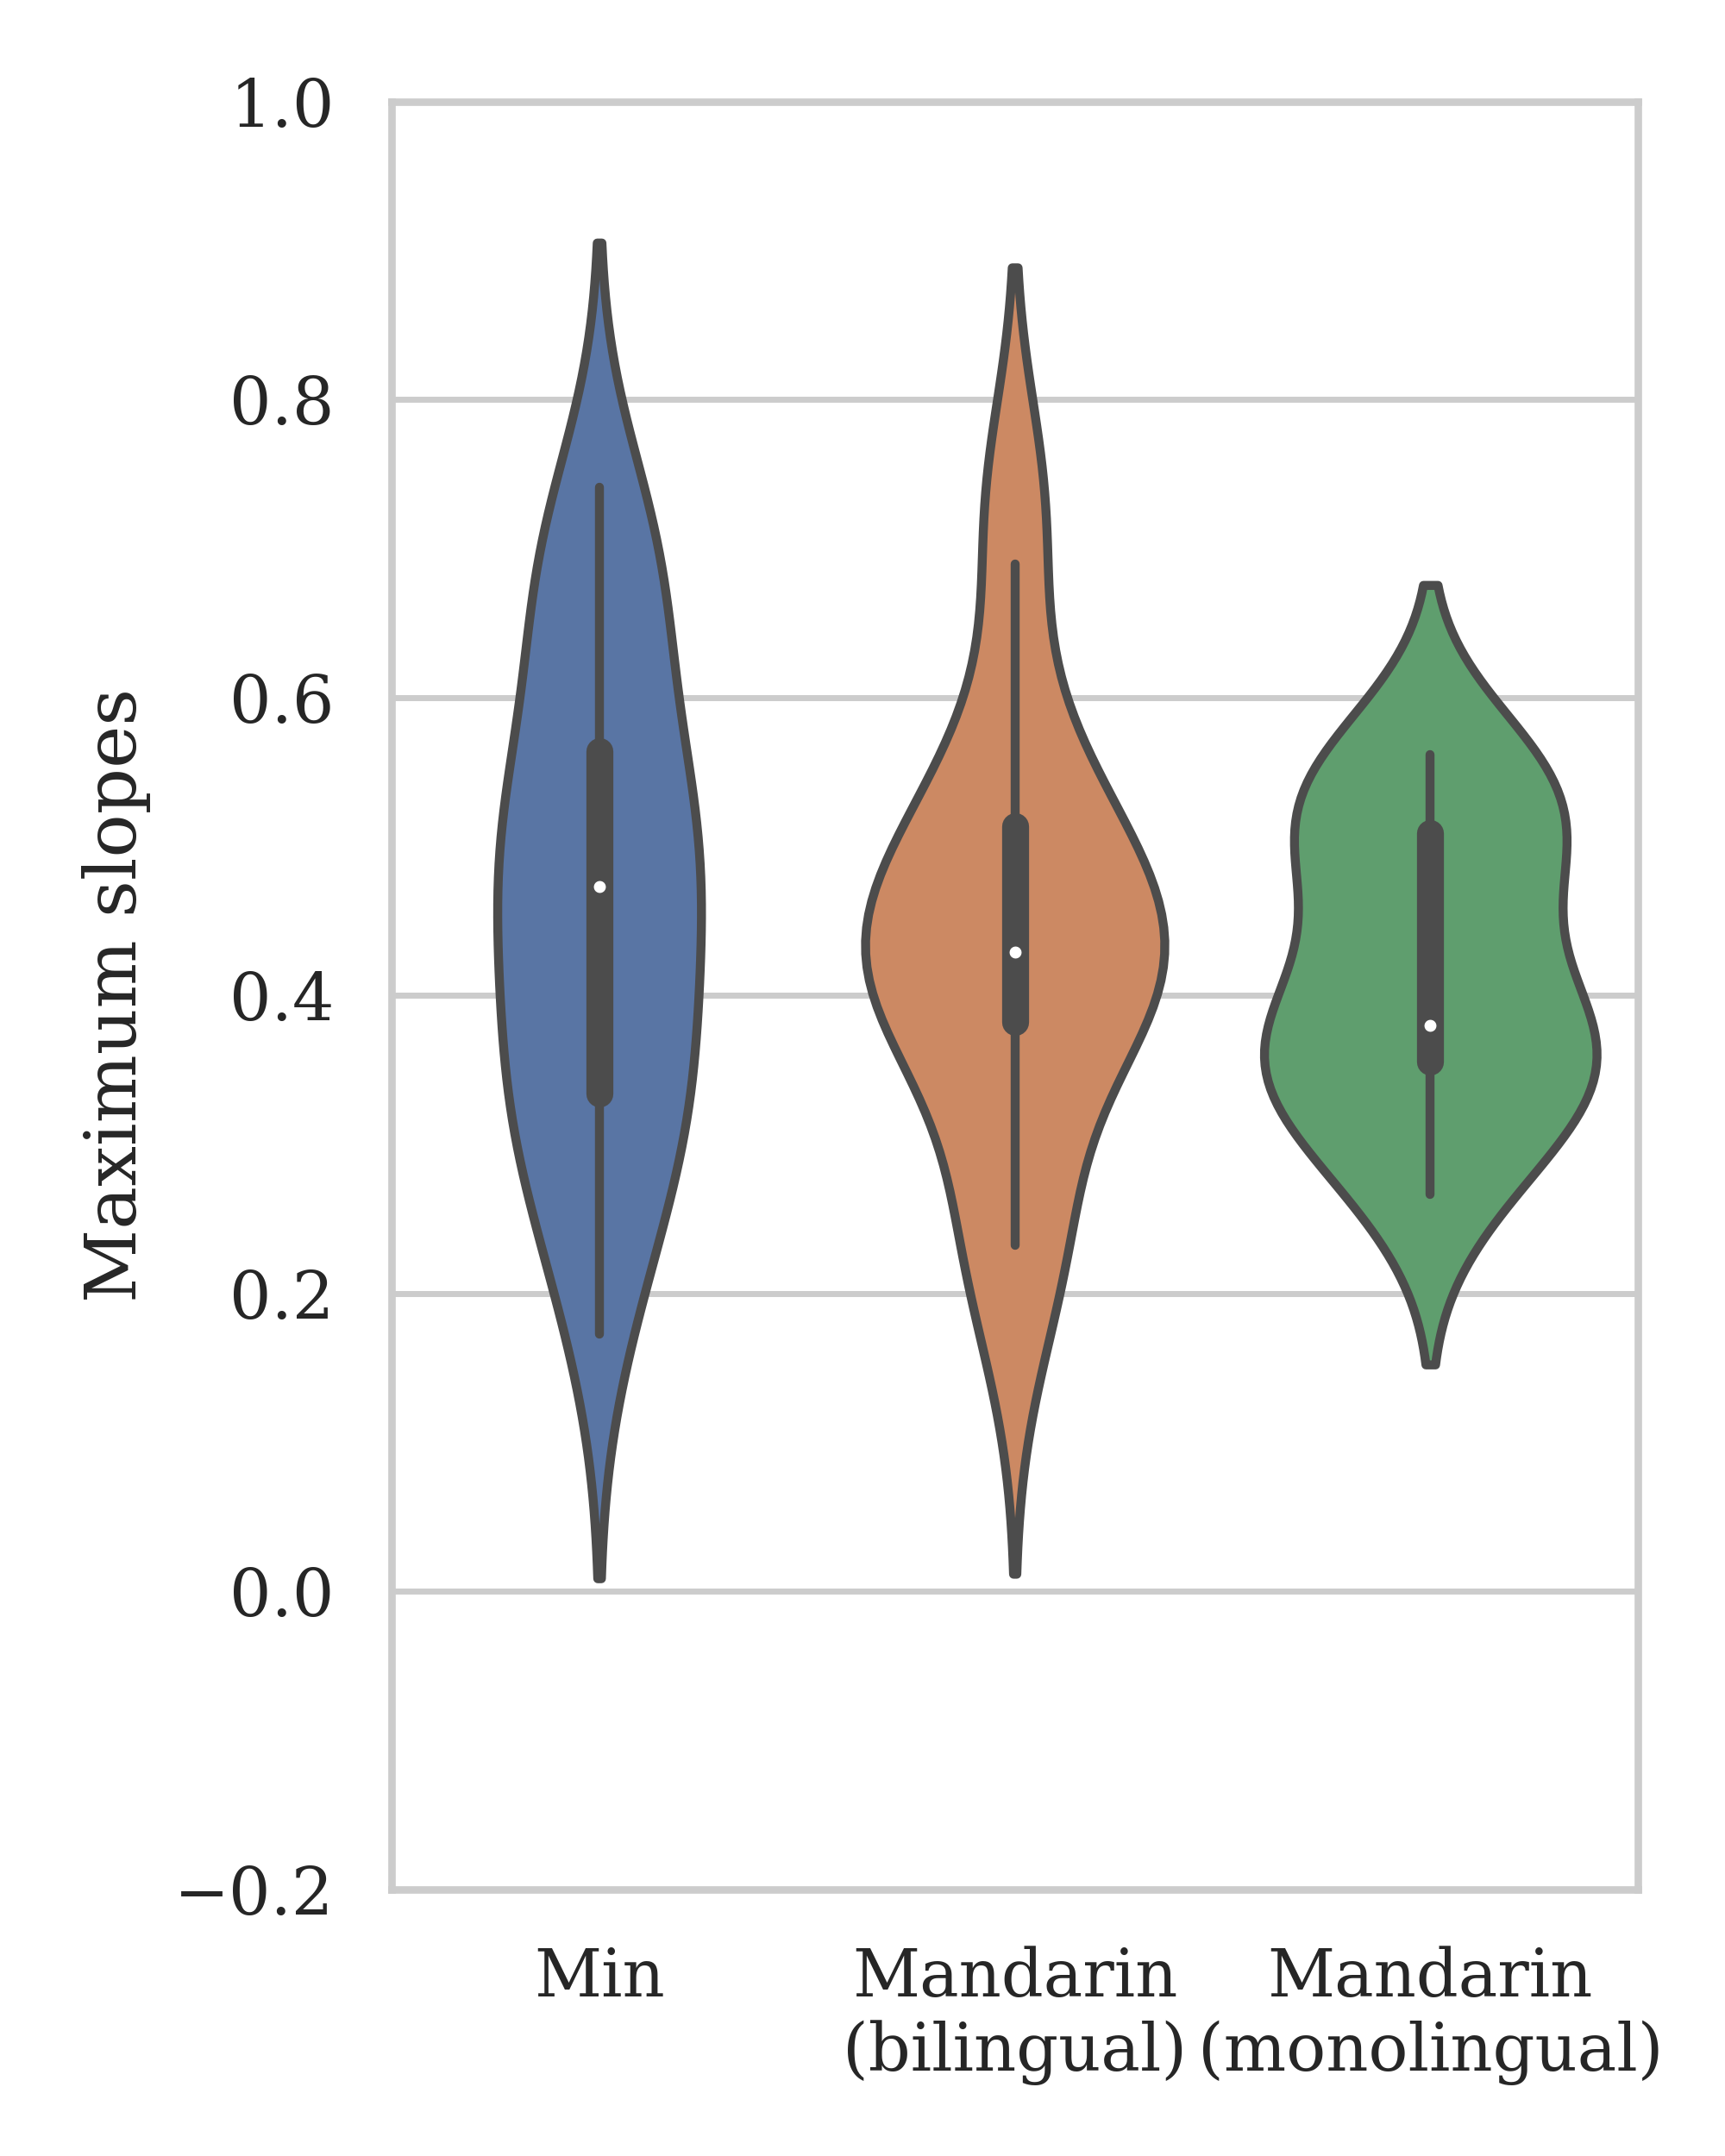
\includegraphics[width=\textwidth]{Figures/E3/Result_51.png}
\end{subfigure}
\hfill
\begin{subfigure}[b]{.49\textwidth}
\centering
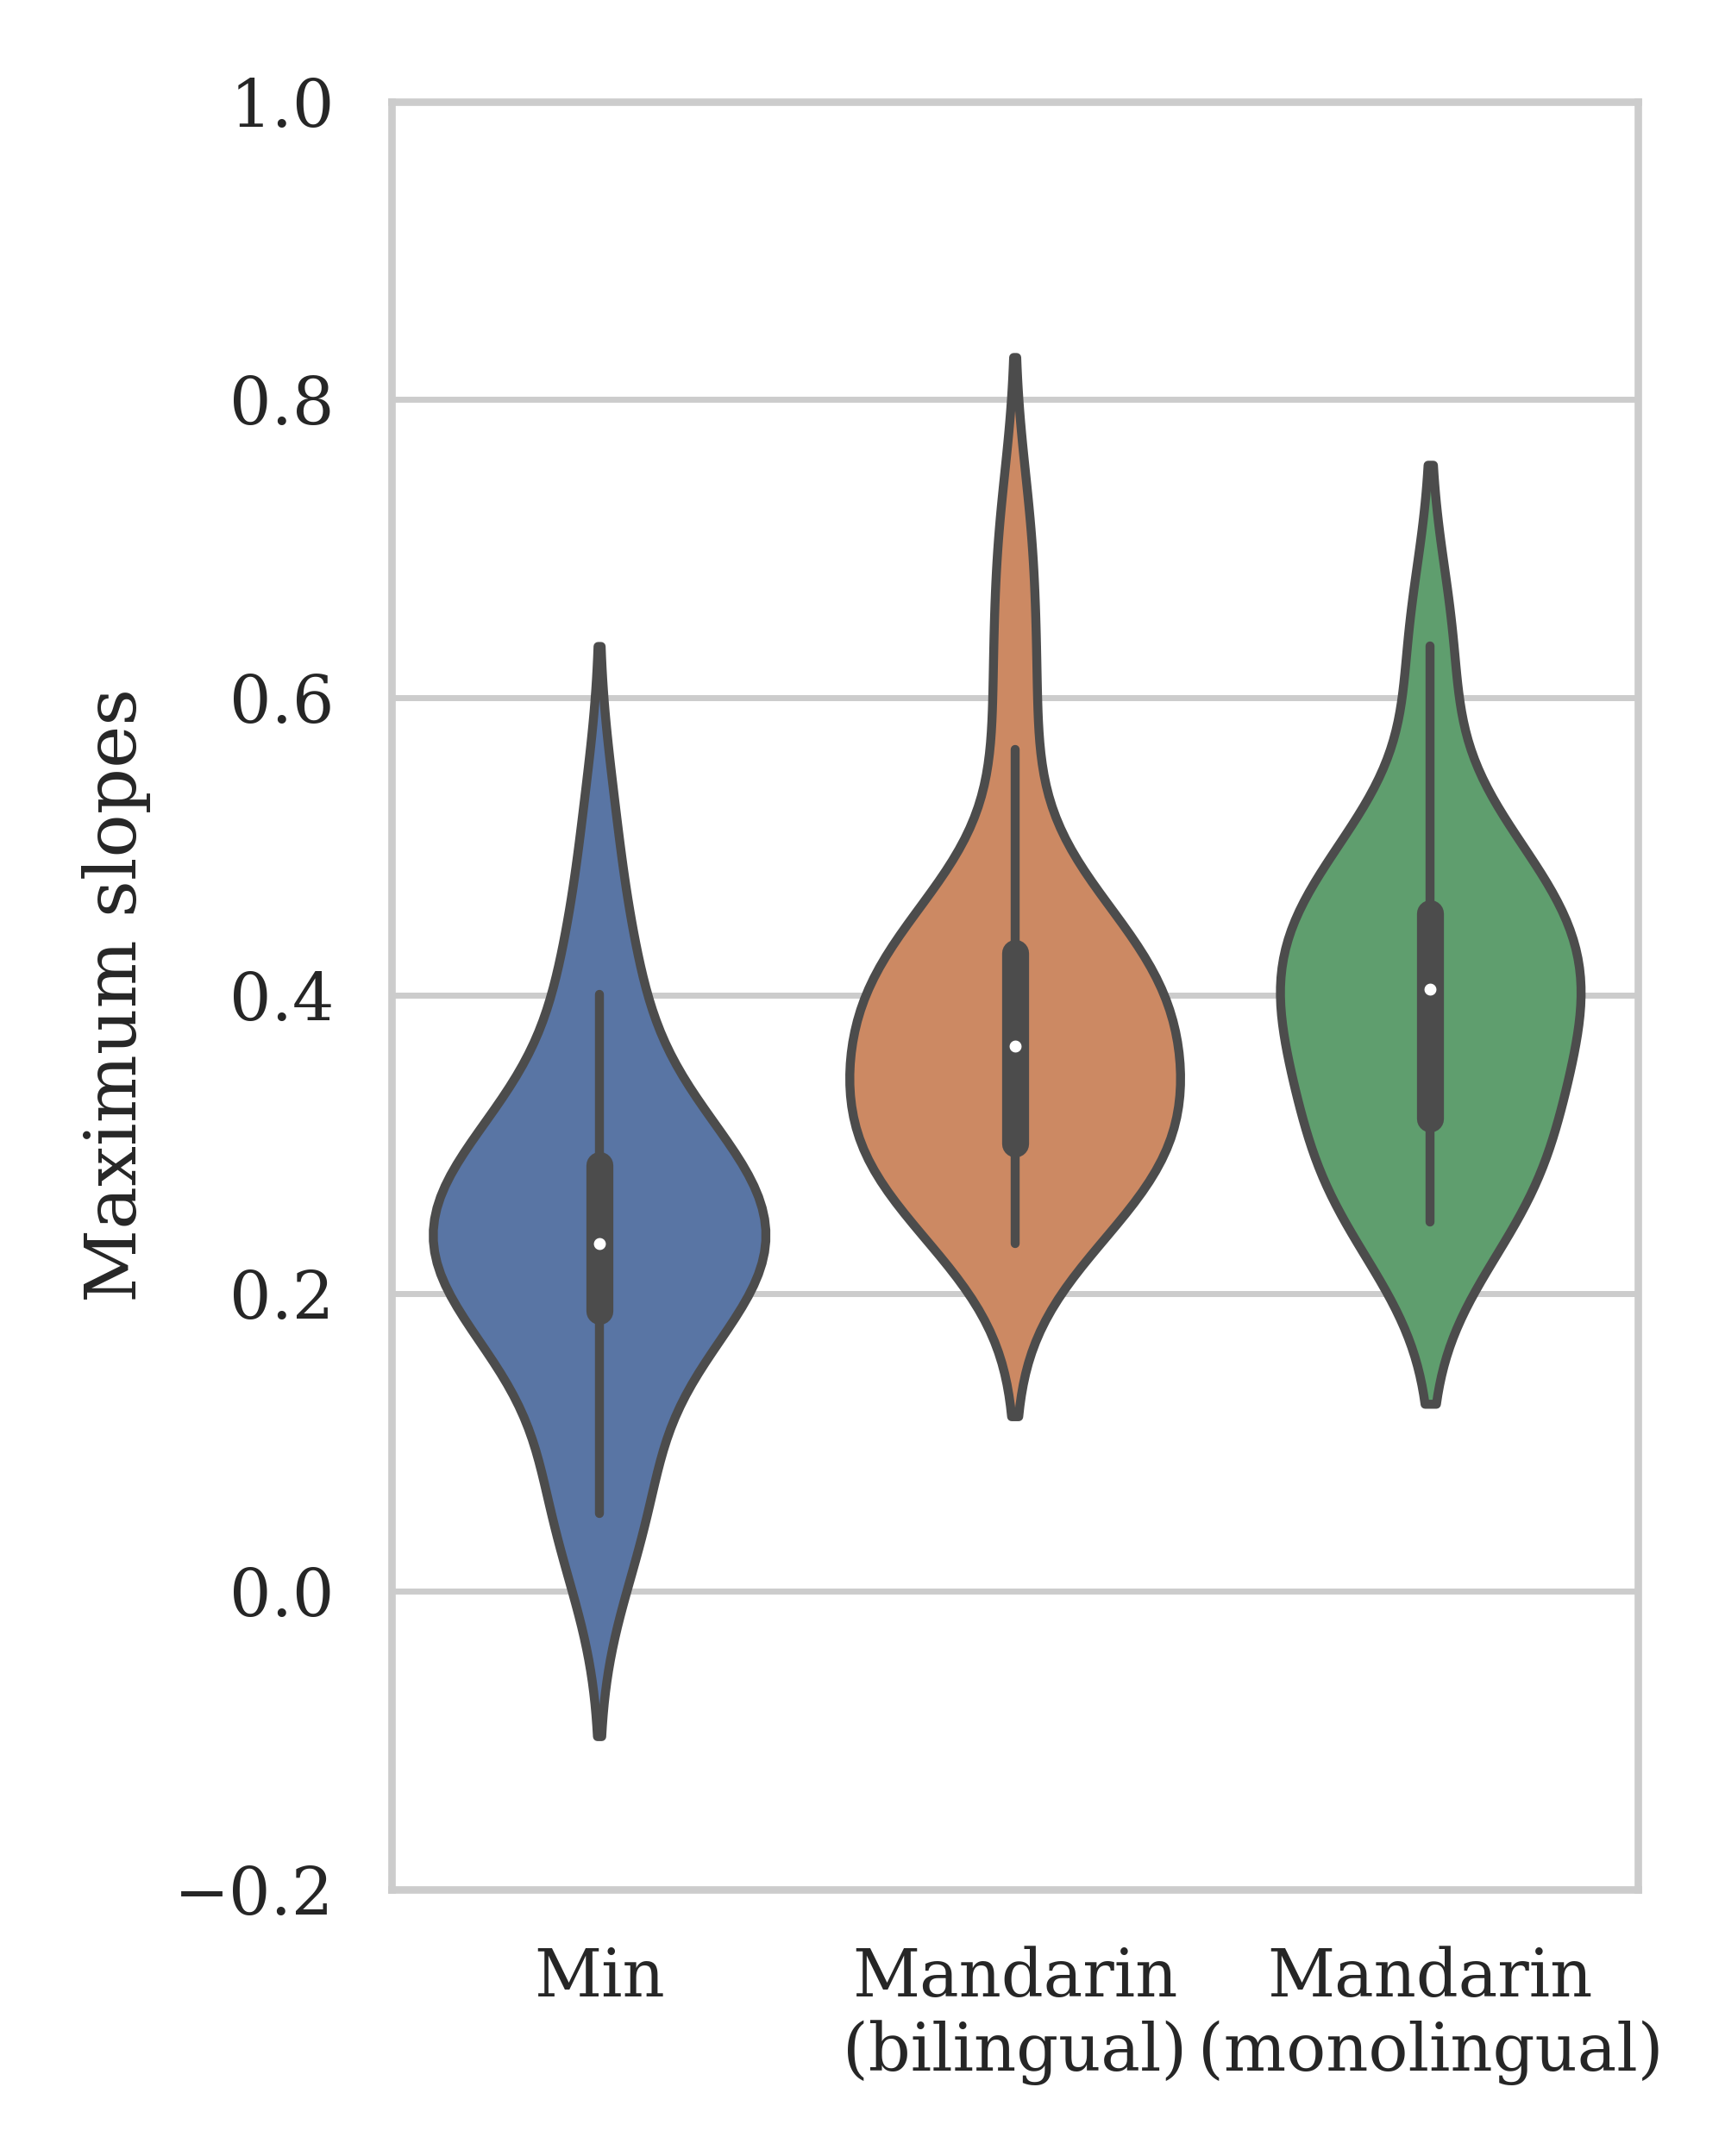
\includegraphics[width=\textwidth]{Figures/E3/Result_21.png}
\end{subfigure}

\caption{Maximum slopes of tone acceptance rate regression lines (left: falling tone; right: low tone).}
\label{Figure:E3BoxPlot}
\end{figure}

\begin{figure}[hbt!]
\centering
\begin{subfigure}[b]{.49\textwidth}
\centering
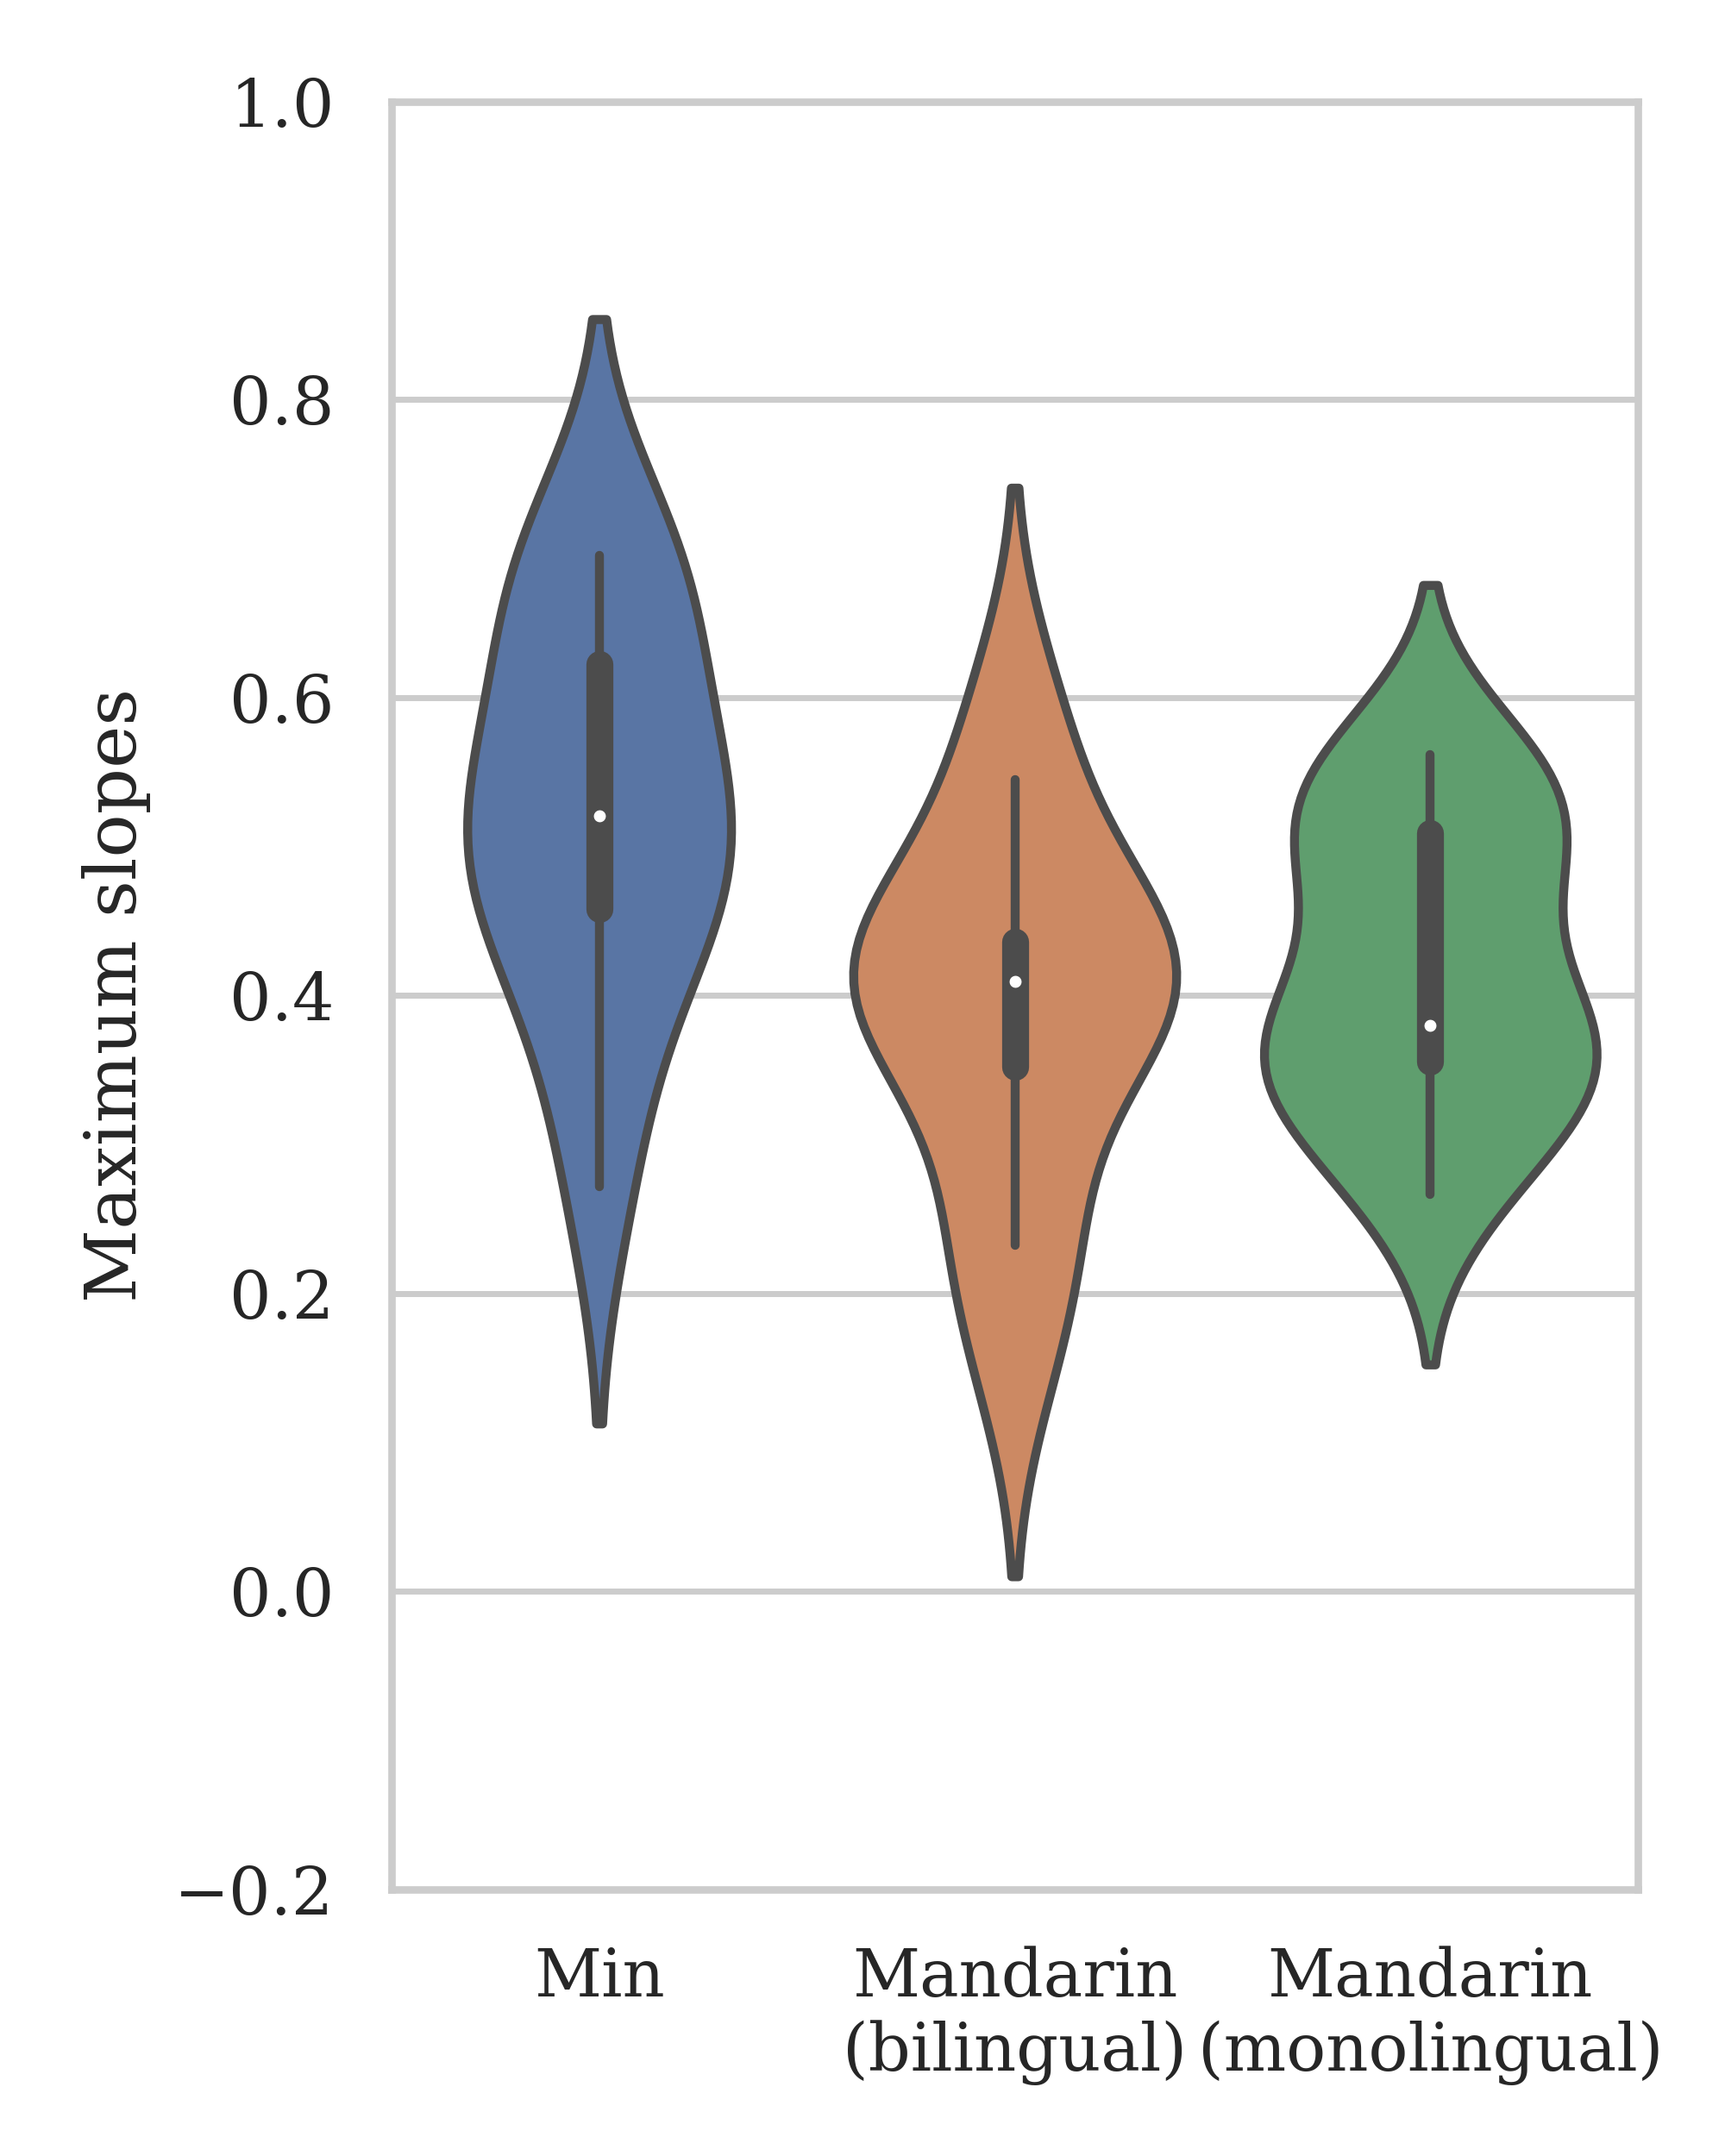
\includegraphics[width=\textwidth]{Figures/E3/Result_51_advanced.png}
\end{subfigure}
\hfill
\begin{subfigure}[b]{.49\textwidth}
\centering
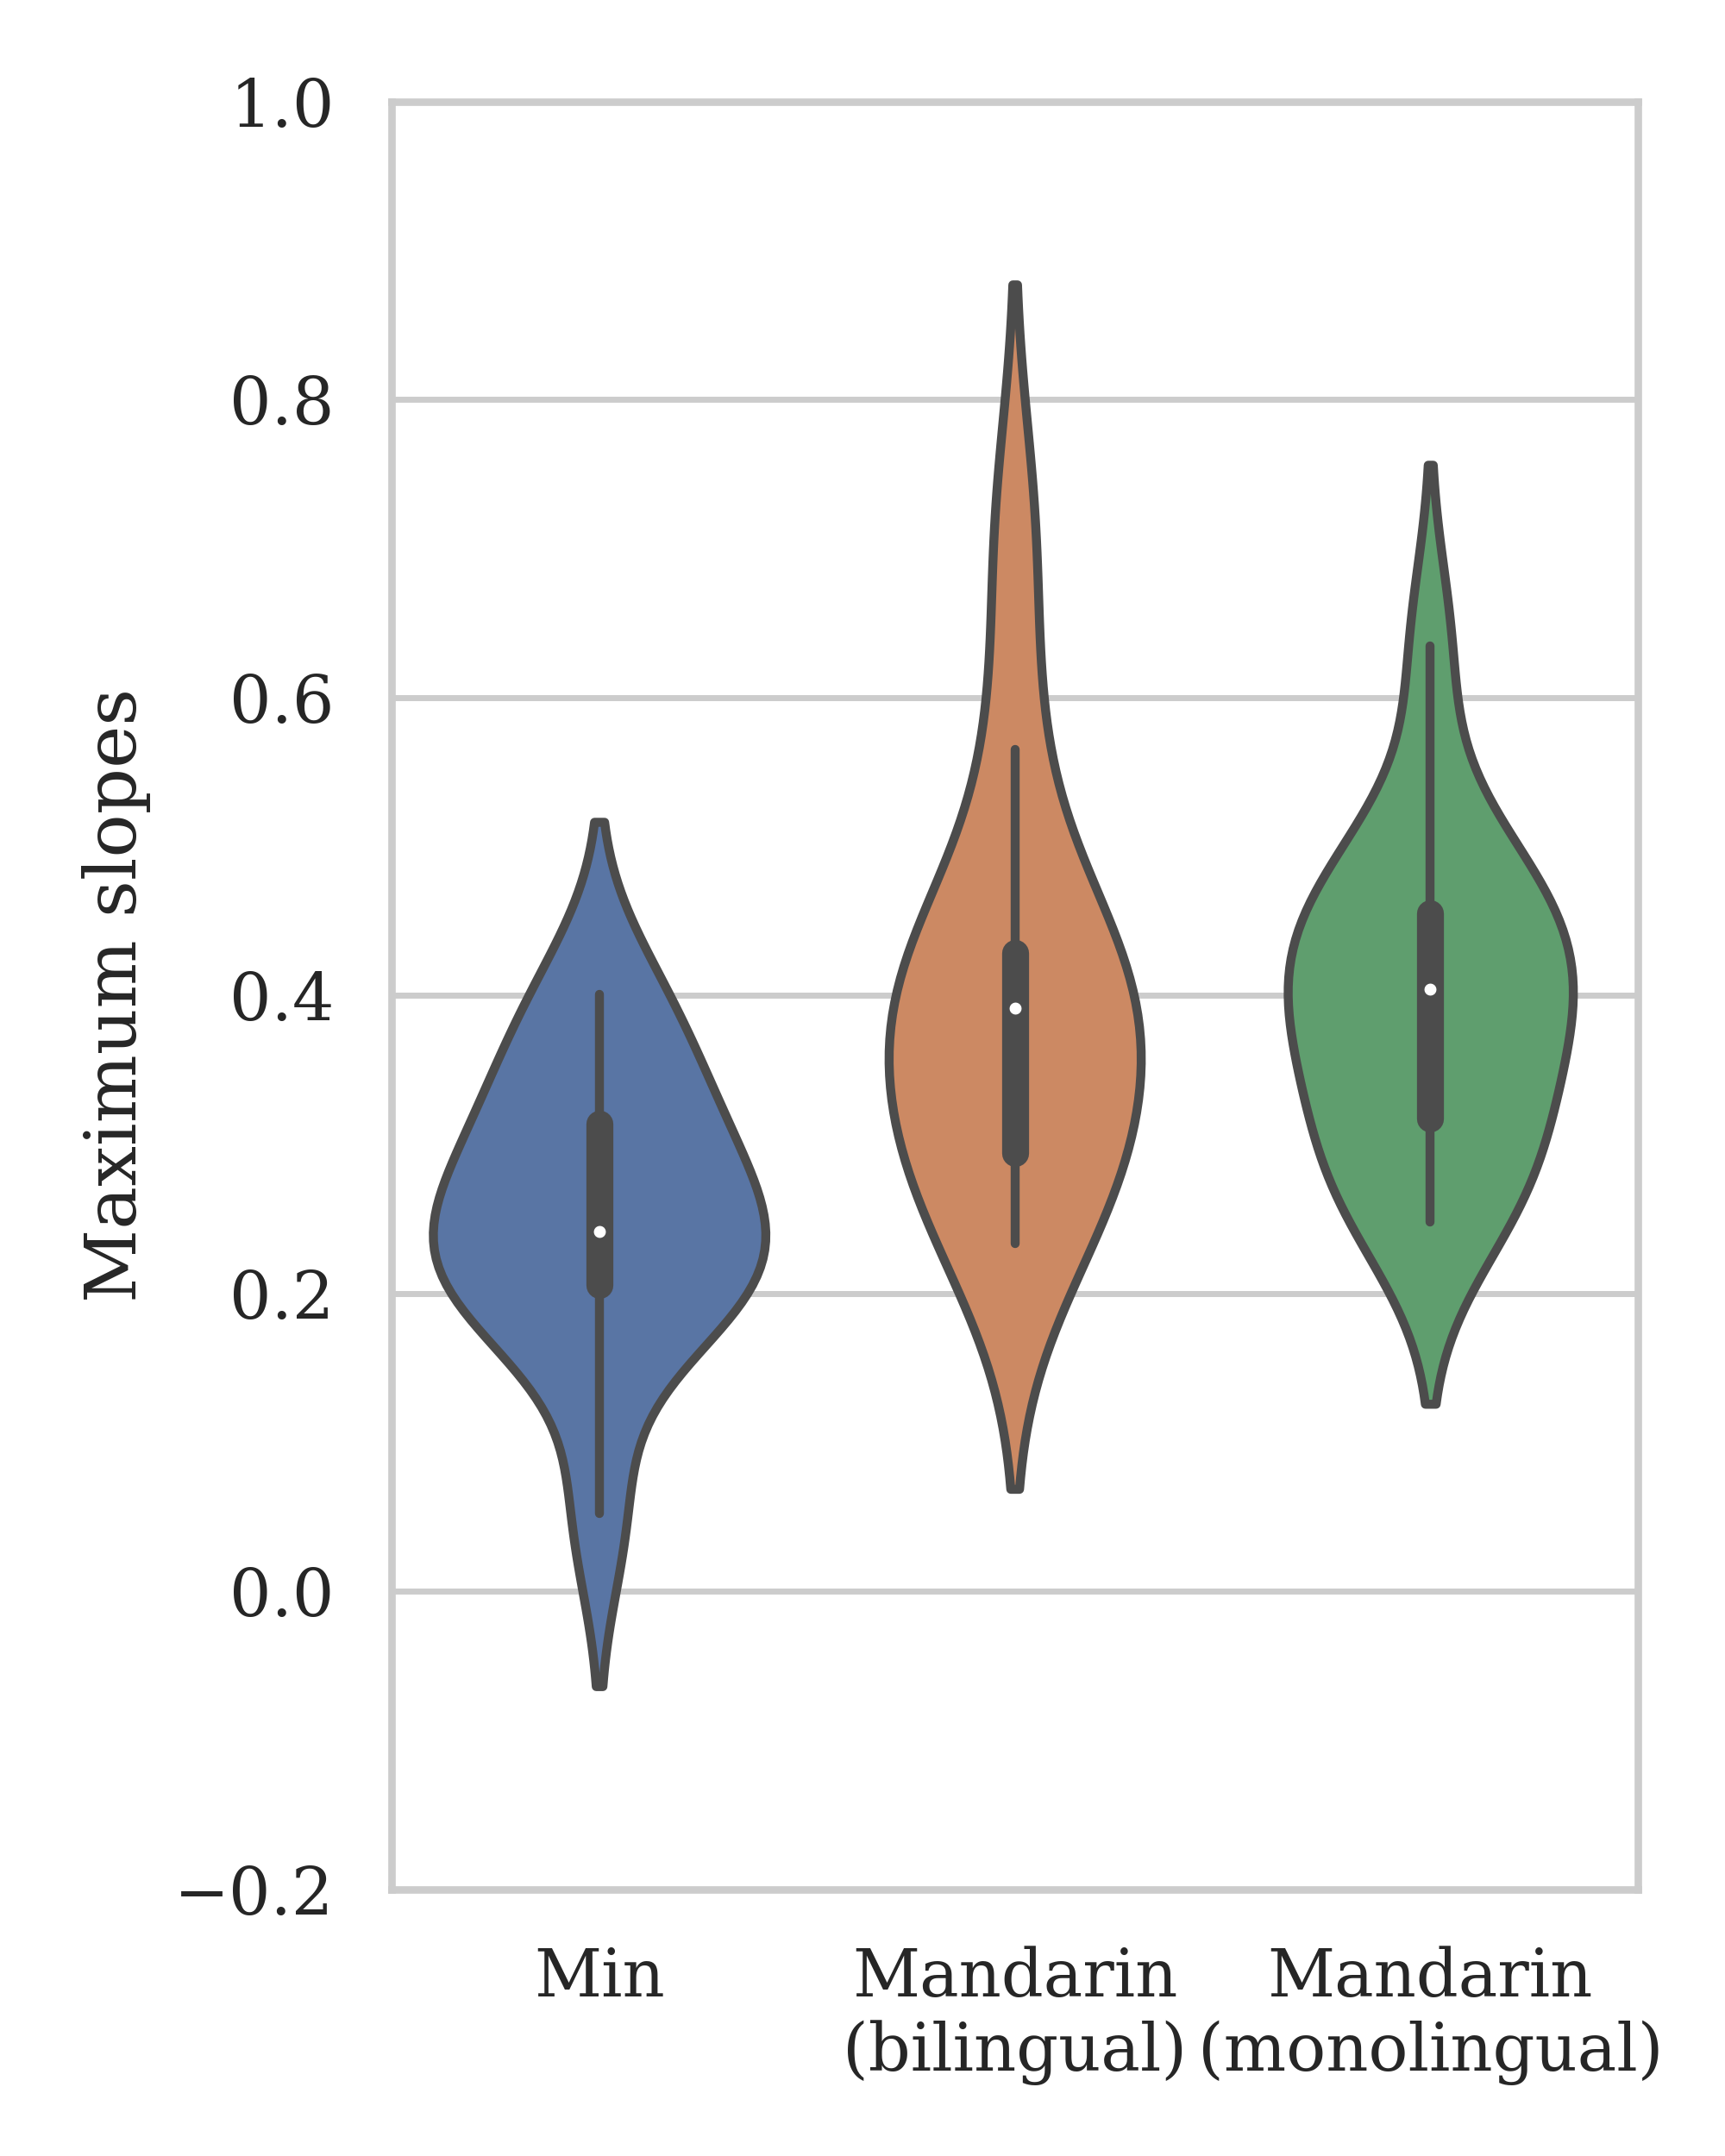
\includegraphics[width=\textwidth]{Figures/E3/Result_21_advanced.png}
\end{subfigure}

\caption{Maximum slopes of tone acceptance rate regression lines (left: falling tone; right: low tone; advanced subjects only).}
\label{Figure:E3BoxPlot}
\end{figure}

%Two one-way ANOVA's were done to examine the differences among the the maximum slopes of the bilingual group's Southern Min and Mandarin regression lines, and the monolingual group's Mandarin regression lines for falling and low tones respectively. For falling tone regression maximum slopes, no significant difference was found (F(2, 62)=.65, p=.52). For low tone regression maximum slopes, at least one of the three language$\times$group combinations were found to be different (F(2, 62)=13.23, p<.001***). A Simple t-test showed that bilingual subjects' Min low tone regression maximum slopes were significantly smaller than monolingual subjects' Mandarin results (p<.001***). A paired t-test revealed such linguistic difference was kept even within the bilingual subjects (p<.05*).
%
%To further investigate whether differences would be found when bilingual subjects were advanced speakers only, other two one-way ANOVA's were done again with the intermediate bilingual group's data taken out. This time, falling tone results were found to be significantly different between at least one of the language$\times$group combinations (F(2, 62)=5.31, p<.05*), and so were the low tone results (F(2, 62)=6.76, p<.01**).

Simple t-tests were done to investigate the differences between the bilingual group's Southern Min results and the monolingual speakers' Mandarin results for the falling tones and low tones, respectively. No significant differences were found between the maximum slopes of bilinguals' Southern Min falling tone and those of their Mandarin counterparts' Mandarin falling tone (p=.33). However, for the low tones, the monolingual group's Mandarin slopes were significantly steeper than the bilingual group's Southern Min slopes (p<.001***).

To further investigate whether differences would be found when bilingual subjects were advanced speakers only. Simple t-tests were also done with the intermediate bilingual group's data taken out. It was revealed that the slope distributions were opposite between monolingual speakers' Mandarin and advanced bilingual speakers' Southern Min. Maximum slopes of the falling tone regressions were larger in the advanced bilingual speakers' Southern Min (p<.05*), while when it turned to the low tone's acceptance, it was the monolingual speaker's Mandarin that had steeper slopes (p<.01**). Recall that in section \ref{section:Experiment3}, it is mentioned that the slopes are taken as indicators of the speakers' strictness on the tone boundaries. This suggests that when the monolingual speakers had stricter low tone boundaries in Mandarin, and that the advanced bilinguals had stricter falling tone boundaries in Southern Min. A paired t-test revealed such linguistic difference was kept even within the bilingual subjects (both p's <.05*).

\section{Summary}
In this section, we have examined tonal coarticulation in Taiwan Mandarin and Taiwan Southern Min, and normalization and tone boundaries in the two languages. It is seen that while Taiwan Mandarin and Taiwan Southern Min exhibited rather similar distribution in terms of tonal coarticulation, Taiwan Southern Min was shown to be less influenced by the normalization effect of tonal coarticulation. Tone boundaries of the falling tone and the low tone in these two languages were also shown to be different. In the next chapter, we will discuss the significances of these discrepancies and of other results that we have seen in this section.

\pagebreak
\chapter{Discussion}

In this chapter, we discuss the results we have seen in the previous chapter, and how they may echo with the research questions posed in chapter \ref{chapter:Introduction}. Specifically, two main tenets are delved into: 1) tonal coarticulation in Taiwan Southern Min and Taiwan Mandarin, 2) interaction between strictness of tone boundaries and normalization for tonal coarticulation. In addition, we will also touch upon the issues regarding the nature of tonal coarticulation and of general versus language-specific perception.

\section{Tonal coarticulation in Taiwan Mandarin and Taiwan Southern Min}

In this section, we talk about the coarticulatory effects of adjacent tones in Taiwan Mandarin and Taiwan Southern Min, and the consistencies as well as discrepancies between this and previous studies.

\subsection{Symmetric tonal coarticulation and final prominence}

As reviewed in section \ref{section:Tonal coarticulation in Taiwan Mandarin and Taiwan Southern Min}, previous studies generally showed an asymmetry of Mandarin tonal coarticulation in both magnitude and directionality. A prevalent belief is that carry-over effects in Mandarin is stronger and assimilatory, while anticipatory effects are weaker and dissimilatory. While strong and assimilatory effects are also found in our data of Taiwan Mandarin, linear-mixed effect models did not show the anticipatory effects to be significantly weaker, and it was also found that these effects are assimilatory just as carry-over effects. This discrepancy of anticipatory effects between our and previous studies is particularly interesting. Comparison with Taiwan Southern Min may shed light on such finding. In both \cite{Peng1997} and this study, anticipatory effects were found to be assimilatory in Taiwan Southern Min. Such symmetry is likewise found in Malaysian Hokkien in \cite{ChangHsieh2012}, where the authors suggest that Southern Min and Hokkien as languages with rich sandhi rules, can be subject to final prominence, a feature that is of less importance in the previous investigated tonal languages where asymmetry exists in tonal coarticulation. It is argued in \cite{ChangHsieh2012} that the typological asymmetry in tonal coarticulation attested in literature may be likely due to the linearity of speech, which results in ``progressive bias'' and in turn favours rightward coarticulation over leftward anticipatory coarticulation. Such bias might be balanced in light of final prominence in Taiwan Southern Min/Malaysian Hokkien, resulting in rather similar distribution between the coarticulations of the two directions. Given the almost identical distributions of the data we have seen in Taiwan Mandarin and Taiwan Southern Min, one is propelled to believe that tonal coarticulation in Taiwan Mandarin might to a certain extent be under the influence of Taiwan Southern Min, and in turn leads to this dialectal difference we see between the data collected in this study and the results in previous researches of Mandarin, where the investigated dialects were all Beijing Mandarin. It is established that Taiwan Mandarin and Taiwan Southern Min as the two major languages in Taiwan, have deep interaction and mutual influence on every linguistic level, including morphosyntax (e.g., \citealp{Li2008}) and phonlogy (e.g., \citealp{ChuangFon2010}; \citealp{Li2010}), and code-switching between the two languages are more than common in Taiwanese society (cf. \citealp{Yang2021}). Scholars including \cite{Her2012} and \cite{Su2018} also argues that Taiwan Mandarin is a highly unique localized variety of Mandarin, under the influence of Taiwan Southern Min and other Taiwanese languages\footnote{\citeauthor{Her2012} even goes as far to say Taiwan Mandarin is a new-born creole  unique to Taiwanese people.}. It is probable that Taiwan Mandarin is affected by the final prominence we observe in Taiwan Southern Min and Malaysian Hokkien.

\section{Tone boundaries and perception of tonal coarticulation}
Another issue that requires attention is the strong effect of tonal coarticulation we see in the Taiwan Southern Min data. As discussed in chapter \ref{chapter:Introduction}, Taiwan Southern Min is a language with 7 lexical tones, with several of them contrasting with each other only in terms of tone value, and having the same tone shapes. This means that tone identification is a much harder task in Taiwan Southern Min than in Taiwan Mandarin. As can be seen in figure \ref{Figure:ToneSpace}, if we plot the tone onsets and offsets of the tones produced in isolation by the subjects, the 95\% confidence intervals largely overlap with each other in Taiwan Southern Min. One might imagine these to be even messier when the tones are coarticulated.
\begin{figure}[hbt!]
\centering
\begin{subfigure}[b]{.8\textwidth}
\centering
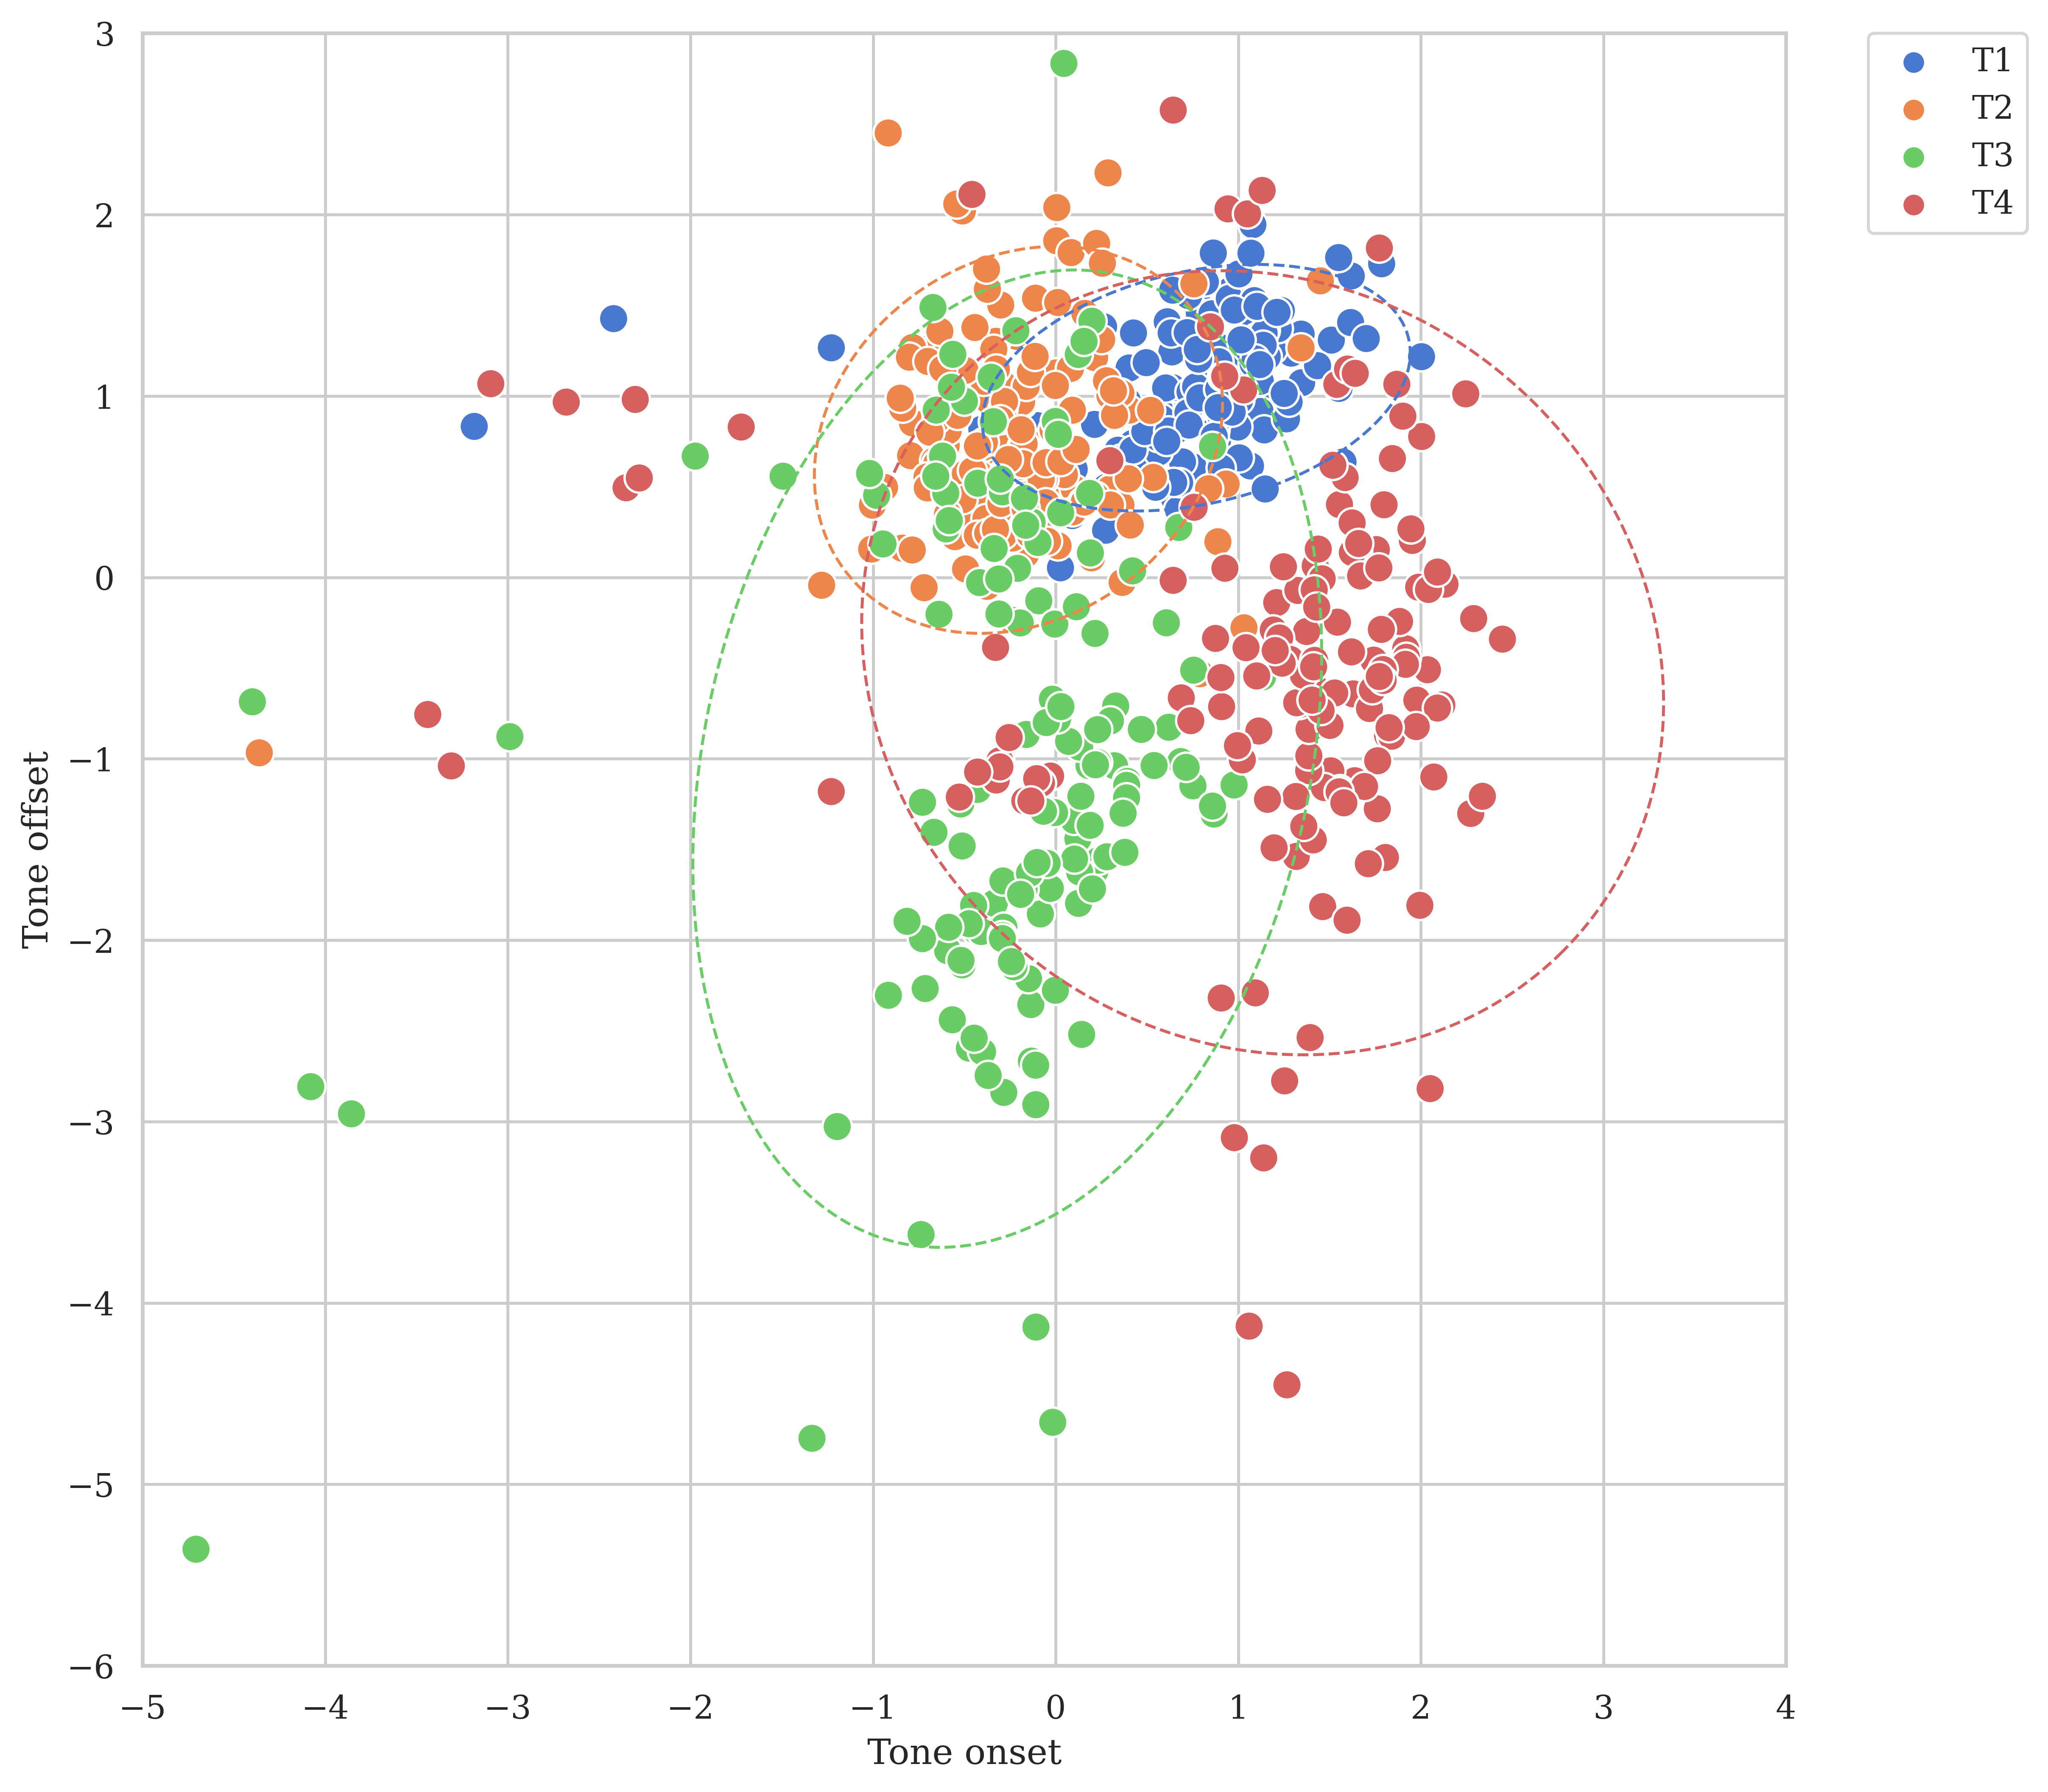
\includegraphics[width=\textwidth]{Figures/Tone_space_Mandarin.png}
\end{subfigure}
\begin{subfigure}[b]{.8\textwidth}
\centering
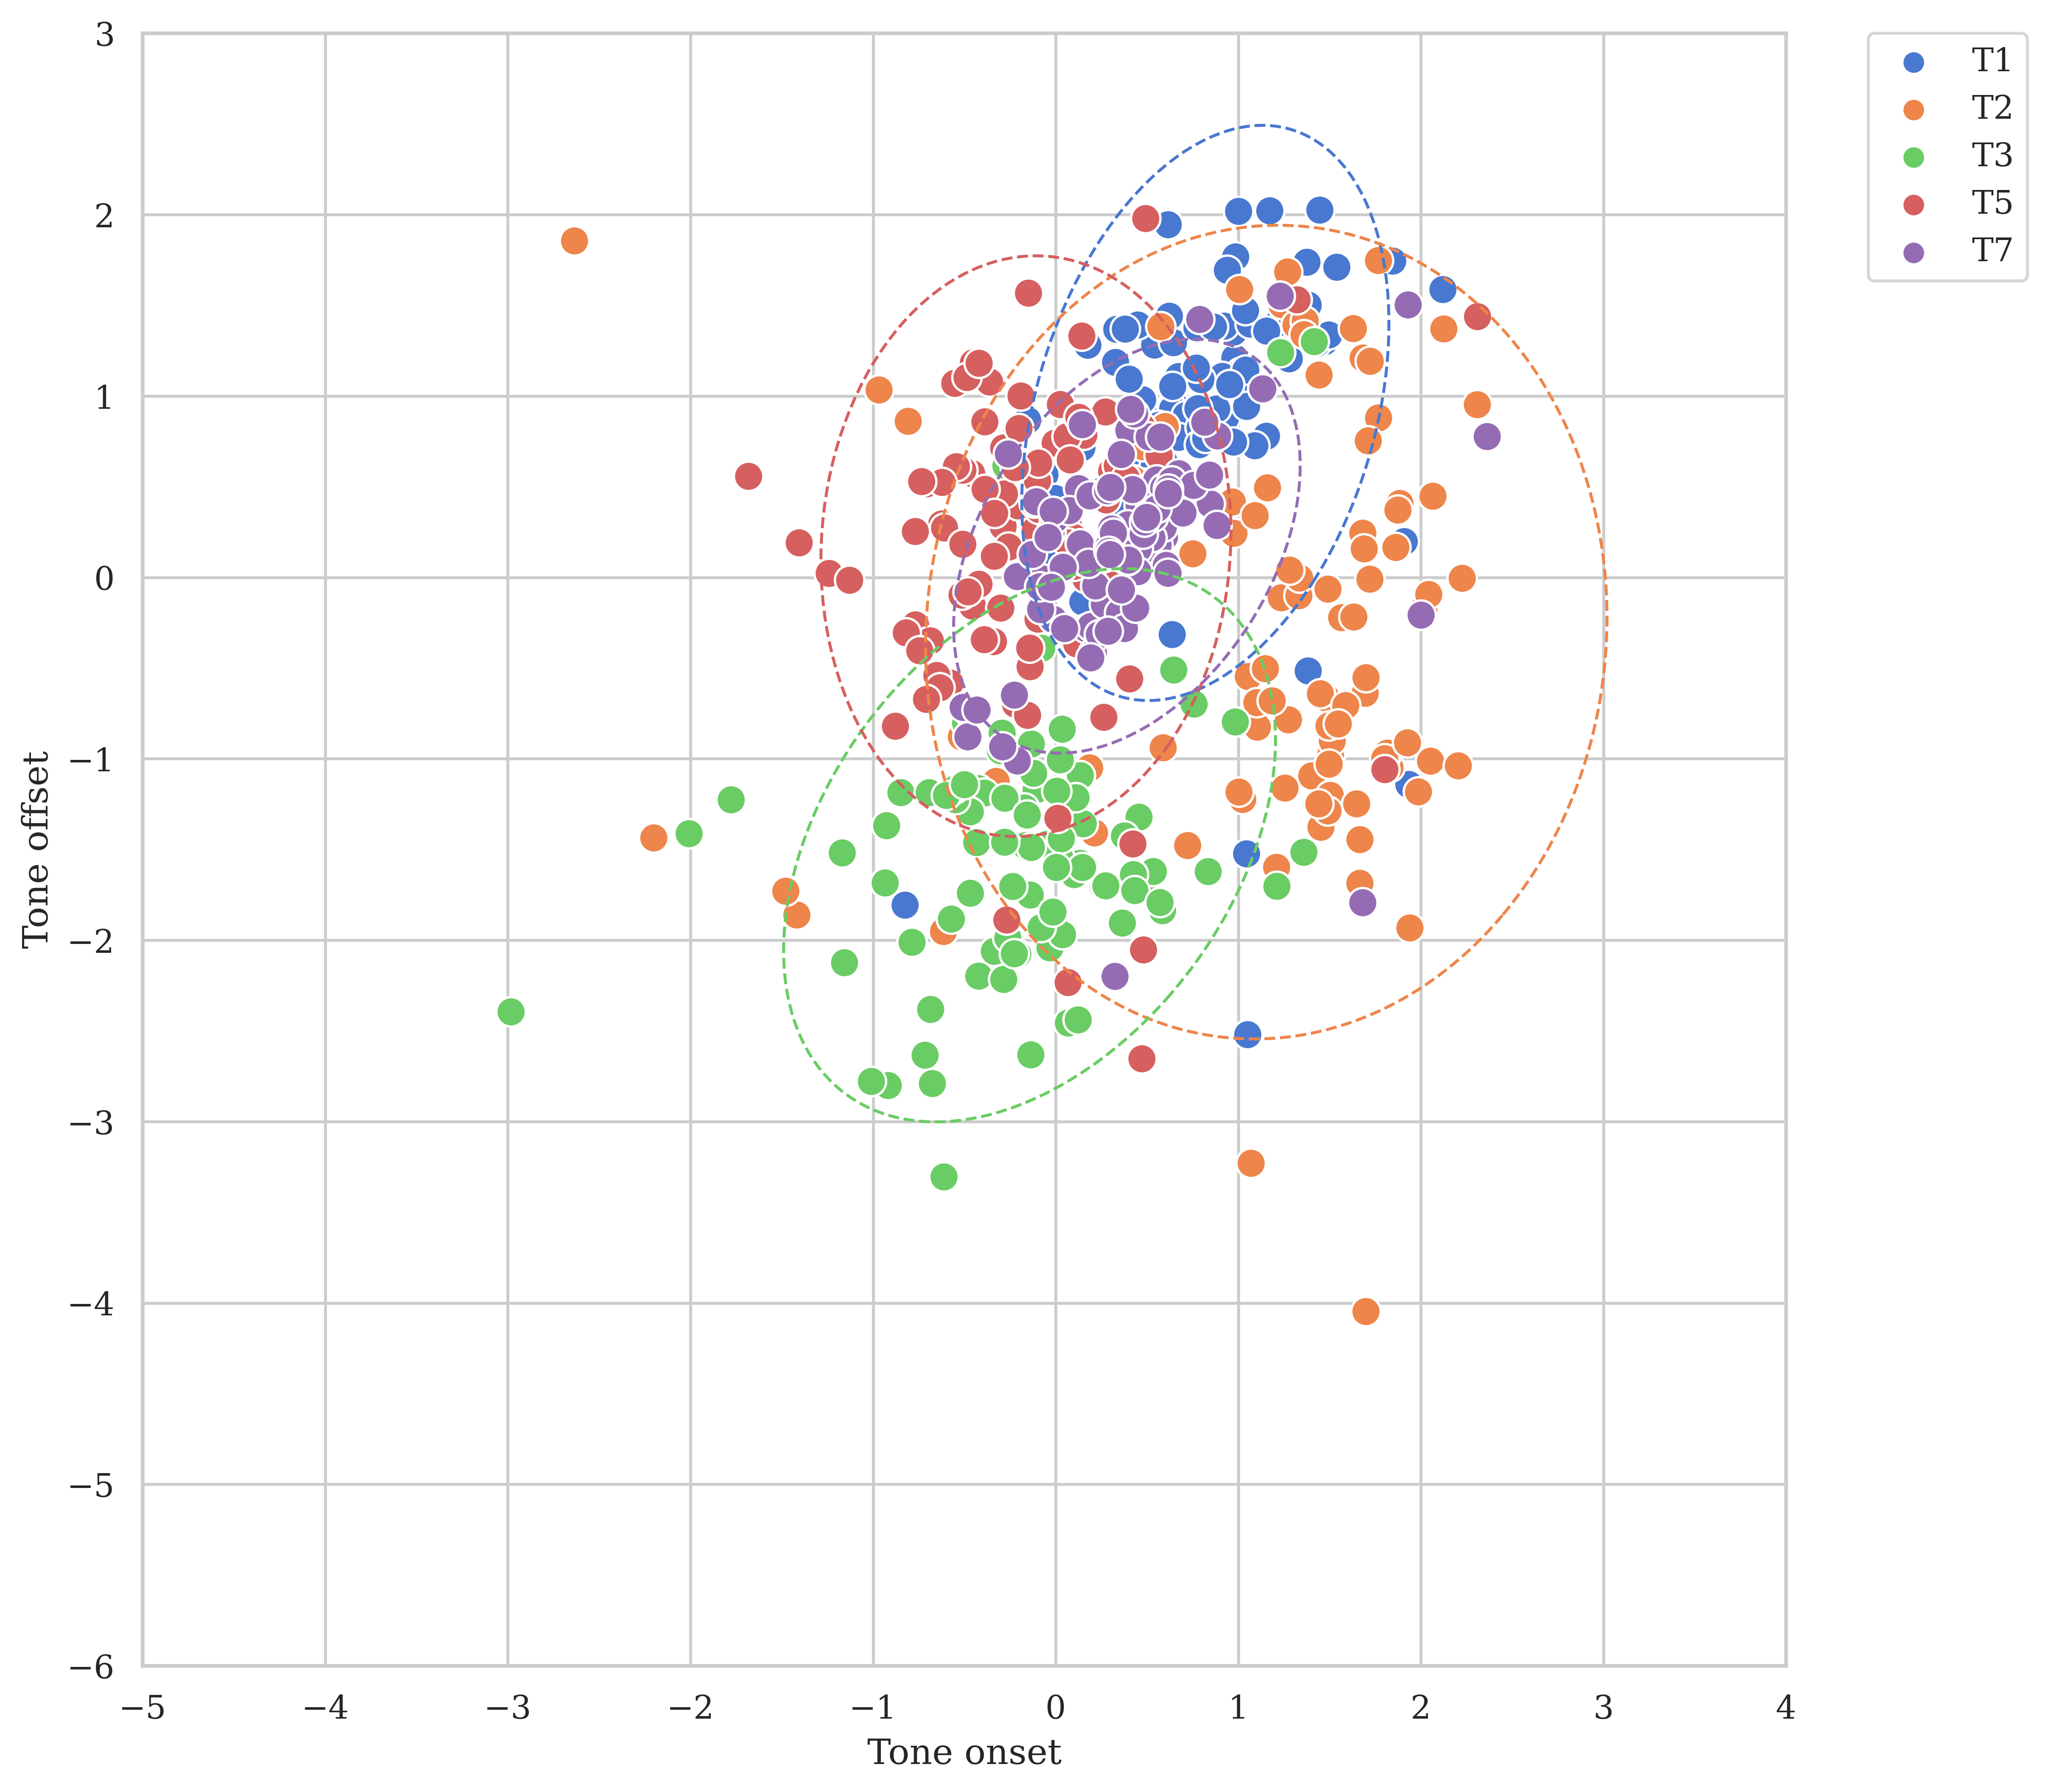
\includegraphics[width=\textwidth]{Figures/Tone_space_Min.png}
\end{subfigure}

\caption{Tonal spaces of Taiwan Mandarin (top) and Taiwan Southern Min (bottom).}
\label{Figure:ToneSpace}
\end{figure}
It is imaginable that tone perception in Taiwan Southern Min would be challenging for listeners when tonal coarticulation is present. Recall that in chapter \ref{chapter:Introduction}, three possible scenarios of tone perception under tonal coarticulation are discussed (cf. figure \ref{Figure:ThreePossibleScenarios}). From the acoustic data in this study, scenario C, where the language has weak tonal coarticulation and can the tones be directly identified without great perturbation seems invalid, as tonal coarticulation is of the same, if not stronger, magnitude in Taiwan Southern Min as in Taiwan Mandarin. This leaves us with two possible scenarios. One is what we have seen in Mandarin (cf. \citealp{Zhangetal2022}), where strong normalization is attested. In both \cite{Xu1994} and \citeauthor{Zhangetal2022}, the perception of coarticulated tones was subject to normalization. Mandarin listeners, whether implicitly or explicitly, enlists the knowledge of pitch variation caused by adjacent tone's F0 values, and make according adjustment in order to retrieve the target that the interlocutor means to produce. While such account suffices to explain the perception of coarticulated tones. It cannot reconcile with the Taiwan Southern Min data we see in this study. In this study, Taiwan Southern Min, though having the same or even stronger tonal coarticulatory effects as Taiwan Mandarin, has significantly weaker normalization effects. Just as mentioned in chapter \ref{chapter:Introduction}, this result is understandable. If Taiwan Southern Min users are to rely only on normalization for tone identification under coarticulation, one would have much more possible candidates to normalize back to than in Taiwan Mandarin. (cf. the perceptual recoverability mentioned in \citealp{Flemming2011}). The weaker normalization effect suggests some other factors are at work for Taiwan Southern Min speakers to facilitate effective communication. It is possible that Taiwan Southern Min is a language that takes on the route B in figure \ref{Figure:ThreePossibleScenarios}, where the speakers have stricter tone boundaries for lexical tones. This scrutiny prevents coarticulated tones from being perceived as another lexical tone at the phonemic level. It is likely for Taiwan Southern Min listeners, a raised low tone that would be taken as an acceptable token of high tone in Taiwan Mandarin would be rejected, and still be perceived as a low tone. This can be illustrated in figure \ref{Figure:ToneAcceptanceIllustration}. 
\begin{figure}[hbt!]
\centering
\begin{subfigure}[b]{.495\textwidth}
\centering
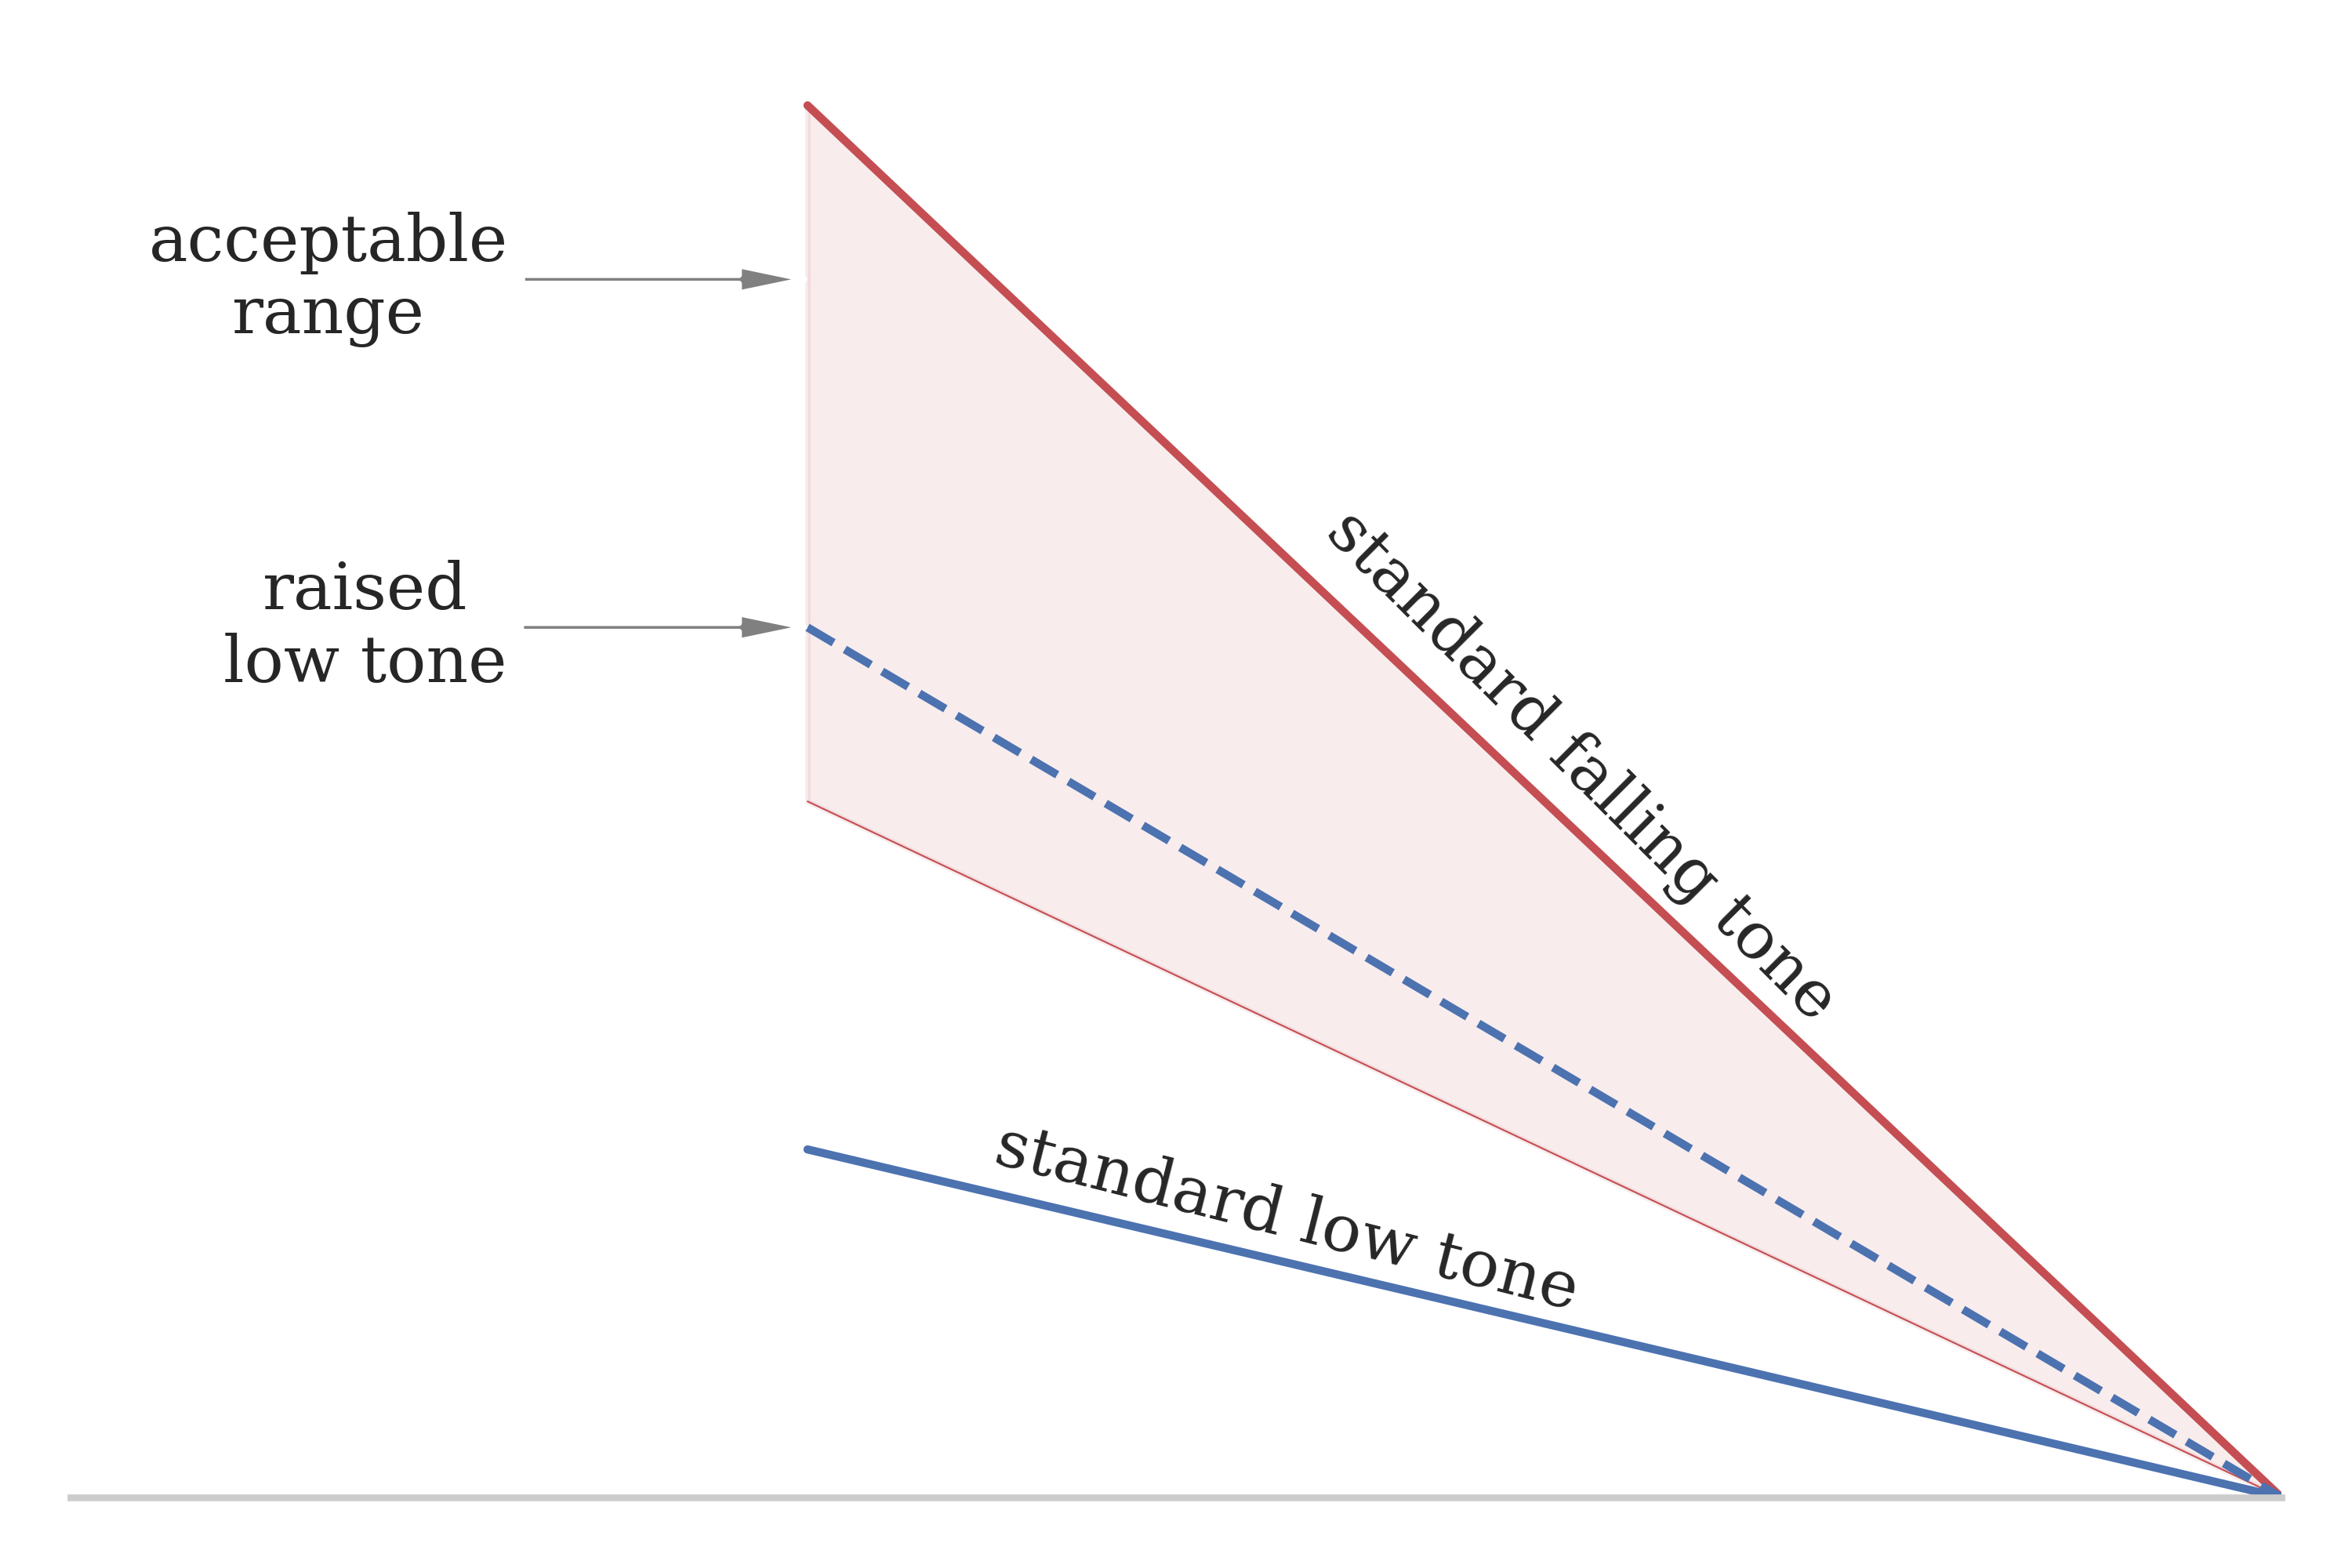
\includegraphics[width=\textwidth]{Figures/Tone_acceptance_illustration_wide.png}
\end{subfigure}
\begin{subfigure}[b]{.495\textwidth}
\centering
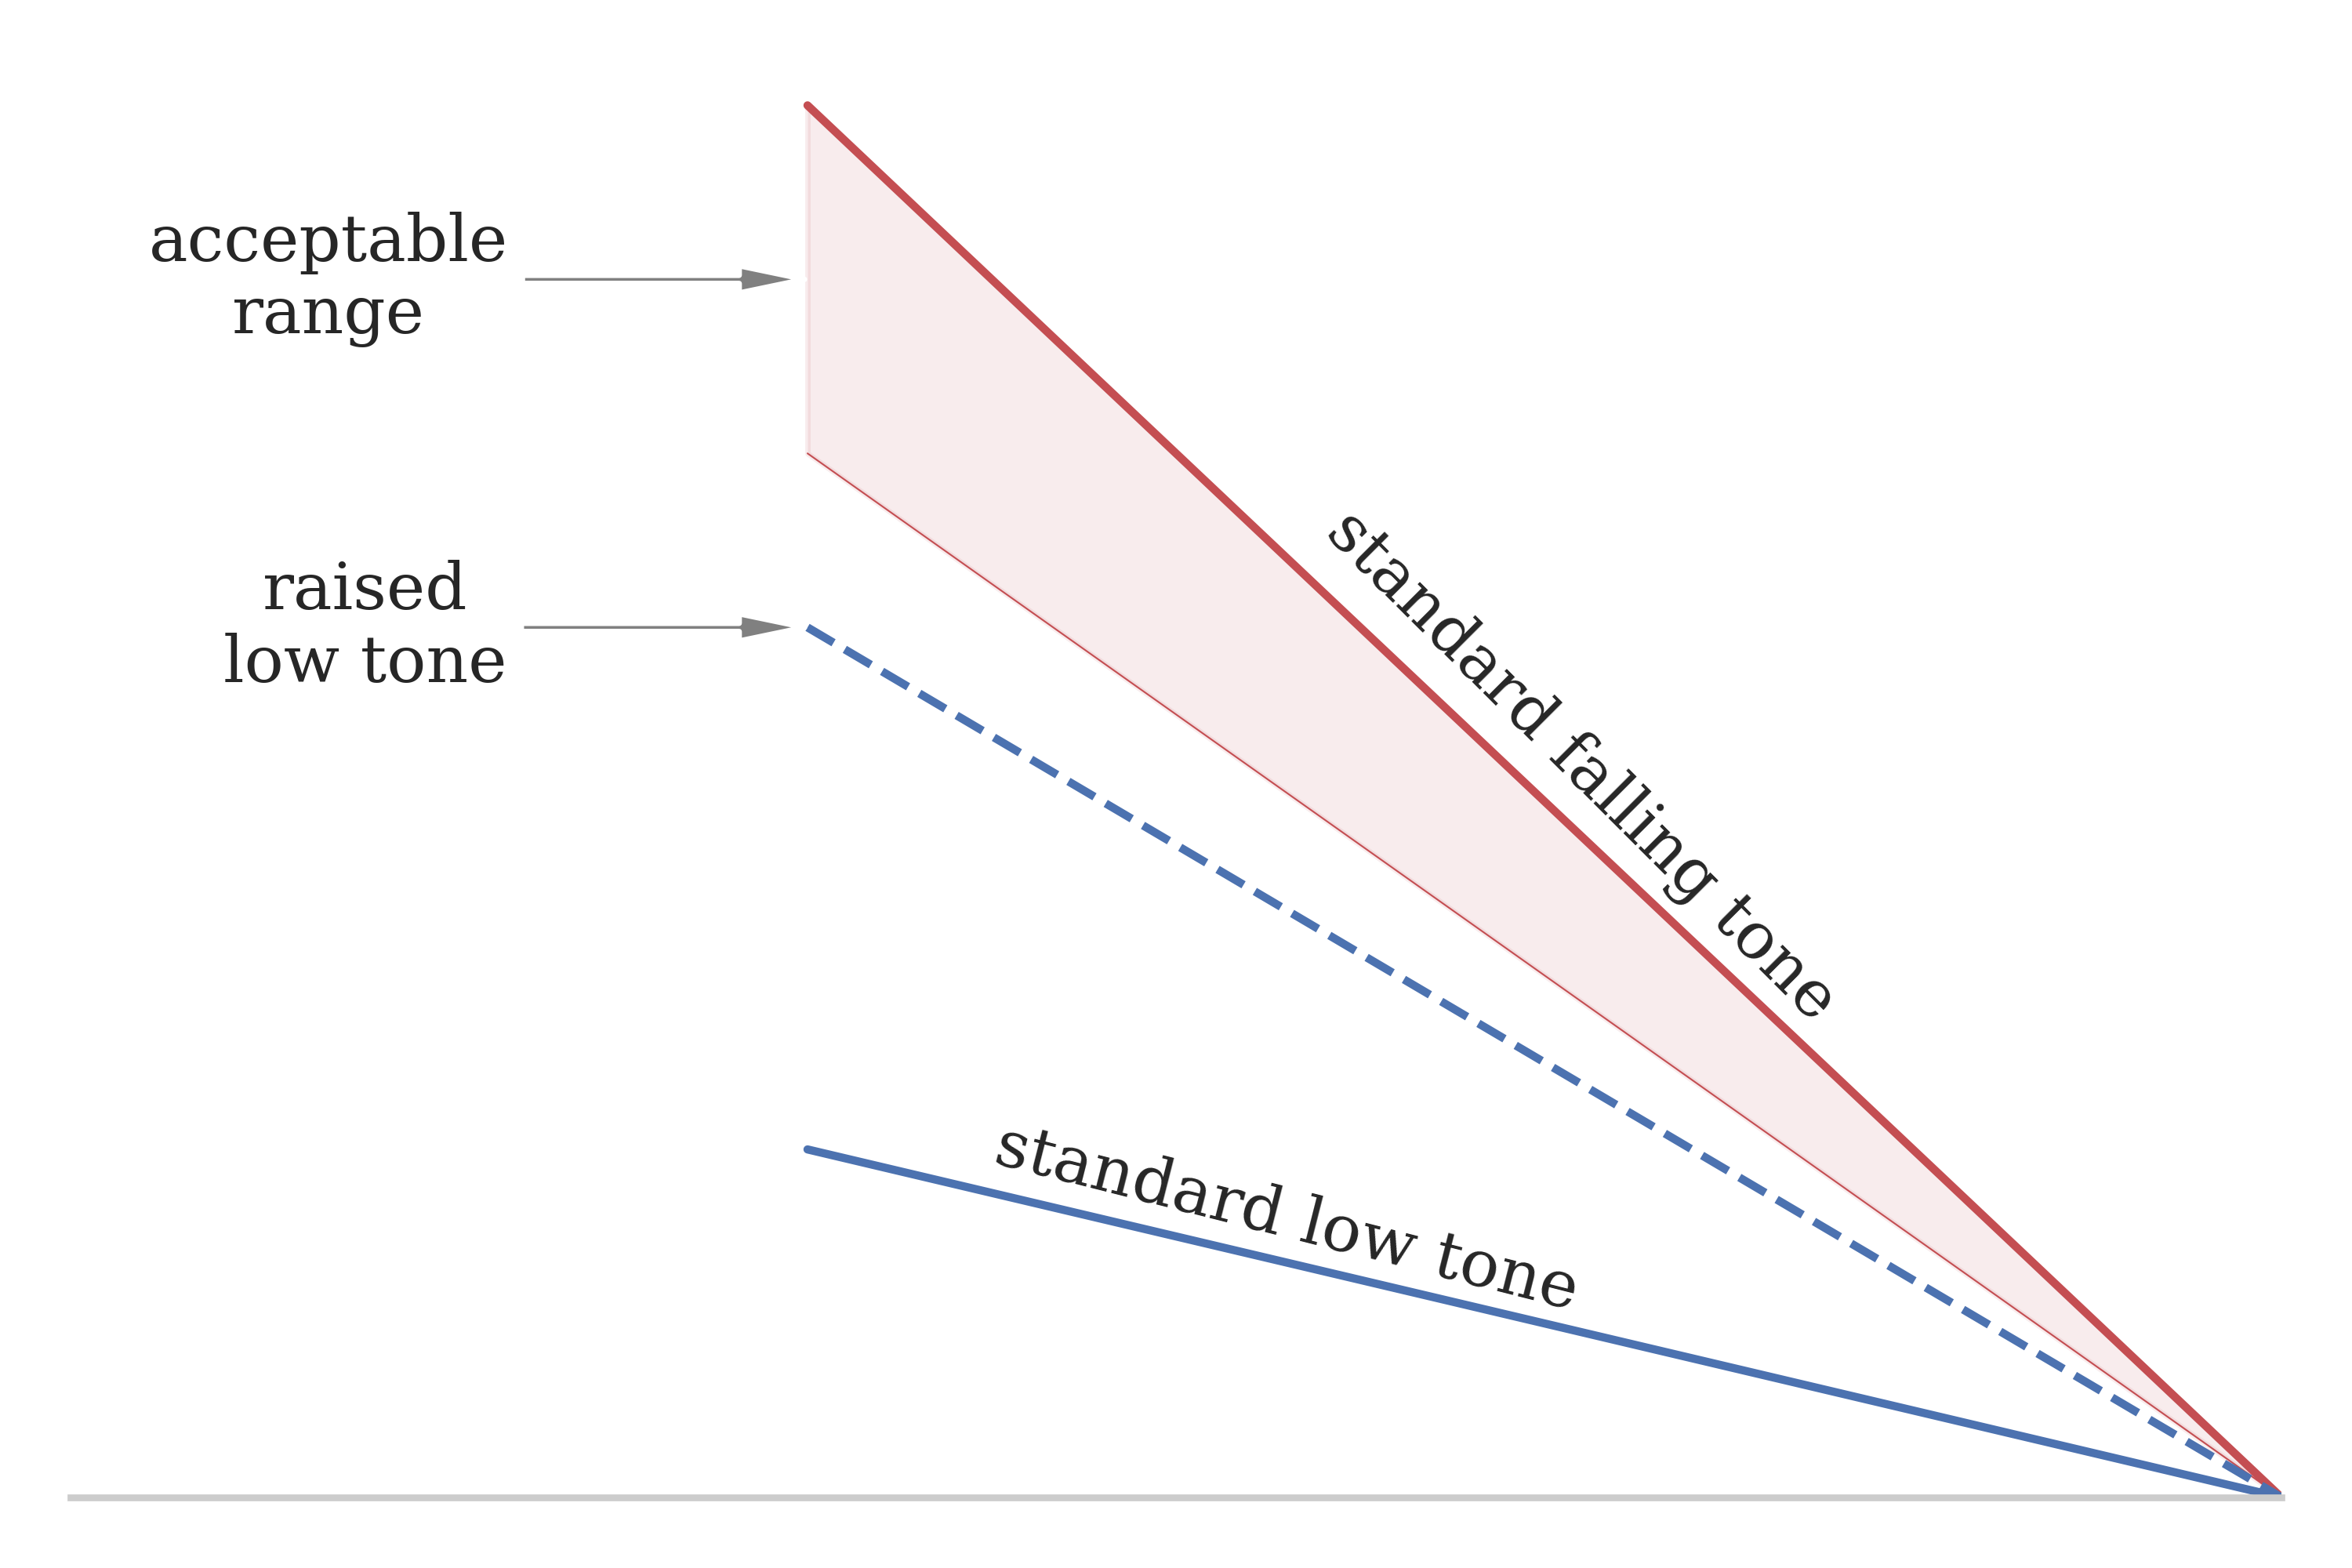
\includegraphics[width=\textwidth]{Figures/Tone_acceptance_illustration_narrow.png}
\end{subfigure}

\caption{Illustrations of wider (left) vs. narrower (right) tone acceptance ranges.}
\label{Figure:ToneAcceptanceIllustration}
\end{figure}
In this case, normalization is less likely, since perceptually, the low tone is never a high tone to begin with. Indeed, if we look at the results of Experiment 3, we see that Taiwan Southern Min subjects had lower tolerances for Taiwan Southern Min falling tone than their Taiwan Mandarin counterparts did for Taiwan Mandarin falling tone. The question is why reversed was found for the low tones. For the low tones, the Mandarin subjects had steeper regression lines. This is likely due to the fact that under sandhi rules, Taiwan Southern Min low tone becomes the falling tone. Though the stimuli was isolated disyllabic words, and the subjects were instructed to imagine the words were produced in isolation, several subjects reported feeling both the low tone versions and falling tone versions to be acceptable for them. This might explain why the boundaries for low tone were not significantly stricter for Taiwan Southern Min subjects as well. That is to say, judging from the results seen in Experiments 2 and 3, Taiwan Southern Min differs from Taiwan Mandarin in that, though both have rather strong tonal coarticulation, the former has stricter tone boundaries that prevents coarticulated tones from being perceived as other lexical tones, while the latter accepts them as good tokens of other lexical tones, and undergoes normalization afterwards.

\section{The nature of tonal coarticulation}
After seeing tonal coarticulations in Taiwan Mandarin and Taiwan Southern Min, a question naturally arises: Is tonal coarticulation a universal trait that occurs naturally as a bio-mechanical result? As argued in chapter \ref{chapter:Introduction} and in the previous section, it is painstaking for a language with large tone inventory to allow for tonal coarticulation. Perception becomes challenging with the already complicated tonal space becoming even messier, and normalization would also be hard considering the multiple possibilities of the target tone. As shown, Taiwan Southern Min listeners had to have stricter tone boundaries to attain successful comprehension. Things would be easier, if tonal coarticulation were absent or weaker. This is, nevertheless, not what we see in Taiwan Southern Min. We see, instead, rather similar coarticulatory effects for both languages. This suggests that such effects might be involuntary, and conditioned by universal constraints. Several studies have entertained this line of thinking. \cite{Haoetal2018}, for instance, attempted to account for tonal coarticulation in Mandarin with articulatory effects. Varying results of coarticulated tones in continuous speech were modeled as factored by competition of attempt to decrease articulatory effects and the prosodic functional need due to requirements such as accentuation. In this case, the variation we see on coarticulated tones are merely byproducts of different prosodic needs. The authors also found that duration could help distinguishing tones with coarticulation and without. This hints that tonal coarticulation is likely influenced by biological mechanism. \cite{Flemming2011} also proposes that certain cross-linguistic universals exist, and it is language-specific variations that interact with such constraints, resulting in the discrepancies we see in languages. While the nature of tonal coarticulation is not the direct tenet of this study. We should at least consider the possibility that tonal coarticulation might be to a certain extent universal across languages.

\section{General perceptual compensation vs. speech-specific normalization}

Another issue that is not the main theme of this study, but is still worth discussing is the debate over whether the normalization we have seen is linguistic or is merely part of the broader general perceptual compensation. This has been debated in past literature. People like \cite{WatkinsMakin1994} and \cite{Zhangetal2022} argue that what is generally believed to be speech-specific normalization can actually still be induced even when the stimuli are non-speech materials. This is what \citeauthor{Zhangetal2022} have found in their study, where higher/lower frequency non-speech stimuli could elicit similar effect in their experiment. However, this effect was significantly weaker than when the stimuli were speech sounds. Even the authors had to admit that linguistic factors had a role to play in what they called ``perceptual compensation''. In our study, linguistic differences were shown to have great effect on the outcome of normalization. Even when the two languages' stimuli had exactly the same F0 values, durations, and intensities, the two language groups showed different degrees of normalization. This strongly hints that such phenomenon is not something common among cognitive systems, but is unique to the linguistic faculty.




%===References===
\pagebreak
\bibliographystyle{apacite}
\bibliography{Citations}


%===Appendices===
\pagebreak
\appendix

% \pagebreak
% \chapter{Additional Files}

% 1. \textattachfile{Figures/E1/Tone_space_Mandarin.html}{\textcolor{hypercolor}{3-D Tonal Space in Taiwan Mandarin}}
% \\
% 2. \textattachfile{Figures/E1/Tone_space_Min.html}{\textcolor{hypercolor}{3-D Tonal Space in Taiwan Southern Min}}

\pagebreak
\chapter{Participant Information}\label{Appendix:ParticipantInfo}

\section{Monolingual group}

\begin{flushleft}
\begin{table}[hbt!]
\begin{tabularx}{\textwidth}{|l||X|X|X|}
\hline
Code&Sex&Age&Hometown\\
\hline
\hline
P3&Female&23&New Taipei\\
\hline
P4&Female&22&New Taipei\\
\hline
P5&Female&24&Taichung\\
\hline
P6&Male&26&New Taipei\\
\hline
P8&Male&20&Taipei\\
\hline
P9&Male&24&Hsinchu\\
\hline
P10&Male&22&Taipei\\
\hline
P11&Female&20&Taipei\\
\hline
P12&Female&24&New Taipei\\
\hline
P13&Female&22&Taipei\\
\hline
P20&Male&27&Taichung\\
\hline
P21&Female&22&Taipei\\
\hline
P22&Male&22&Taipei\\
\hline
P33&Female&22&New Taipei\\
\hline
P40&Female&21&Taipei\\
\hline

\end{tabularx}
\end{table}
\end{flushleft}

\pagebreak
\section{Intermediate bilingual group}

\begin{flushleft}
\begin{table}[hbt!]
\begin{tabularx}{\textwidth}{|l||X|X|X|X|}
\hline
Code&Sex&Age&Hometown&Southern Min Fluency\\
\hline
\hline
P2&Female&22&Tainan&6\\
\hline
P15&Female&22&Tainan&5\\
\hline
P16&Female&26&Nantou&7\\
\hline
P17&Male&20&Yunlin&6\\
\hline
P18&Female&21&Tainan&6\\
\hline
P19&Female&22&Taichung&3\\
\hline
P23&Female&20&New Taipei&4\\
\hline
P24&Male&22&Tainan&7\\
\hline
P26&Female&25&Kaohsiung&7\\
\hline
P27&Female&22&Taichung&7\\
\hline
P29&Female&24&Taichung&6\\
\hline
P30&Male&20&Hsinchu&4\\
\hline
P31&Male&23&Taichung&6\\
\hline
P34&Female&21&Taipei&6\\
\hline
P38&Female&21&Kaohsiung&6\\
\hline
P41&Male&25&Changhua&4\\
\hline
P43&Female&24&New Taipei&7\\
\hline

\end{tabularx}
\end{table}
\end{flushleft}

\section{Advanced bilingual group}

\begin{flushleft}
\begin{table}[hbt!]
\begin{tabularx}{\textwidth}{|l||X|X|X|X|}
\hline
Code&Sex&Age&Hometown&Southern Min Fluency\\
\hline
\hline
P1&Male&26&Chiayi&10\\
\hline
P7&Female&27&Tainan&8\\
\hline
P14&Female&21&Tainan&8\\
\hline
P25&Female&20&Taoyuan&8\\
\hline
P28&Male&24&Taichung&10\\
\hline
P32&Female&23&Tainan&8\\
\hline
P35&Male&21&Taipei&8\\
\hline
P36&Female&21&Chiayi&8\\
\hline
P37&Male&20&New Taipei&8\\
\hline
P39&Male&20&Chiayi&9\\
\hline
P42&Female&24&Kaohsiung&9\\
\hline

\end{tabularx}
\end{table}
\end{flushleft}

\pagebreak
\chapter{Stimuli for Experiment 1}\label{Appendix:StimuliforExperiment1}

\section{Taiwan Mandarin stimuli}

\begin{flushleft}
\begin{table}[hbt!]
\begin{tabular}{|l||l|l|l|l|l|}
\hline
 & T1 (55) & T2 (35) & T3 (21) & T4 (51) & Isolated\\
 \hline\hline
\multirow{3}{*}{T1 (55)} & 邀約 & 幽靈 & 邀舞 & 衣物 & 屋 \\
 & /\tip{jaw.4E}/ & /\tip{joU.liN}/ & /\tip{jaw.u}/ & /\tip{i.u}/ & /\tip{u}/ \\
 &`invitation' & `ghots' & `to invite to dance' & `clothes' & `house' \\
\hline
\multirow{3}{*}{T2 (35)} & 牙醫 & 魷魚 & 游泳 & 猶豫 & 無 \\
 & /\tip{ja.i}/ & /\tip{joU.y}/ & /\tip{joU.joN}/ & /\tip{joU.y}/ & /\tip{u}/ \\
 &`dentist' & `squid' & `to swim' & `to hesitate' & `no' \\
\hline
\multirow{3}{*}{T3 (21)} & 女巫 & 有餘 & 營養 & 網路 & 五 \\
 & /\tip{ny.u}/ & /\tip{joU.y}/ & /\tip{iN.jAN}/ & /\tip{wAN.lu}/ & /\tip{u}/ \\
 &`witch' & `more than' & `more than' & `the Internet' & `five' \\
 \hline
\multirow{3}{*}{T4 (51)} & 夜鶯 & 誤移 & 誘餌 & 藥物 & 物 \\
 & /\tip{jE.iN}/ & /\tip{u.i}/ & /\tip{joU.\textrhookschwa}/ & /\tip{jaw.u}/ & /\tip{u}/ \\
 &`nightingale' & `to move by mistake' & `bait' & `medicine' & `thing' \\
\hline
\end{tabular}
\end{table}
\end{flushleft}

\pagebreak
\section{Taiwan Southern Min stimuli}

\begin{flushleft}
\begin{table}[hbt!]
\begin{tabularx}{\textwidth}{|X||X|X|X|X|X|X|X|X|}
\hline
 & T1 (55) & T2 (51) & T3 (21) & T5 (35) & T7 (33)  & Isolated\\
 \hline\hline
\multirow{3}{*}{T1 (55)} & 烏貓 & 阿母 & 哀怨 & 阿娘 & 因為 & 亞 \\
 & /\tip{O.njAw}/ & /\tip{a.bu}/ & /\tip{aj.wan}/ & /\tip{a.nja}/ & /\tip{in.wi}/ & /\tip{a}/\\
 &  `black cat' & `Mom' & `to be pittiful' & `Mom' & `because' & `Asia'\\
\hline
\multirow{3}{*}{T2 (51)} & 按呢 & 母語 & 滿意 & 理由 & 美麗 & 仔 \\
 & /\tip{an.ne}/ & /\tip{bu.gi}/ & /\tip{mwa.i}/ & /\tip{li.ju}/ & /\tip{bi.le}/ & /\tip{a}/\\
 &  `as such' & `mother tongue' & `to be satisfied' & `excuse' & `beautiful' & `diminu-tive'\\
\hline
\multirow{3}{*}{T3 (21)} & 暗安 & 懊惱 & 落落 & 愛人 & 向望 & 暗 \\
 & /\tip{am.an}/ & /\tip{Aw.nAw}/ & /\tip{law.law}/ & /\tip{aj.dzin}/ & /\tip{\s{N}.bAN}/  & /\tip{am}/\\
 &  `good evenning' & `to regret' & `loose' & `lover' & `hope' & `dark'\\
\hline
\multirow{3}{*}{T5 (35)} & 牛奶 & 麻l\'au & 無愛 & 明年 & 眠夢& 麻 \\
 & /\tip{gu.liN}/ & /\tip{mwa.law}/ & /\tip{bo.aj}/ & /\tip{me.ni}/ & /\tip{bin.bAN}/ & /\tip{ba}/\\
 &  `milk' & `mualau' & `to dislike' & `next year' & `to dream' & `numb'\\
\hline
\multirow{3}{*}{T7 (33)} & 內奶 & 袂b\'ai & 願意 & 未來 & 下面 & 罵 \\
 & /\tip{laj.liN}/ & /\tip{bwe.baj}/ & /\tip{gwan.i}/  & /\tip{bi.laj}/ & /\tip{e.bin}/ & /\tip{ma}/\\
 &  `inner tube' & `not bad' & `to be willing' & `future' & `below' & `to scold'\\
\hline
\end{tabularx}
\end{table}
\end{flushleft}


\pagebreak
\chapter{Stimuli for Experiment 2}\label{Appendix:StimuliforExperiment2}

\section{Taiwan Mandarin version}
\begin{flushleft}
\begin{table}[hbt!]
\begin{tabularx}{\textwidth}{|l||X|X|}
\hline
 & T3 (21) & T4 (51)\\
 \hline
 \hline
\multirow{3}{*}{T1 (55)} & 發火 & 發貨 \\
& /\tip{fa.hwo}/&/\tip{fa.hwo}/\\
& `to get angry' & `to send out delivery'\\
\hline
\multirow{2}{*}{T2 (35)} & 獨子 & 獨自 \\
& /\tip{tu.ts1}/&/\tip{tu.ts1}/\\
& `only son' & `alone'\\
\hline
\multirow{2}{*}{T4 (51)} & 破解 & 破戒\\
& /\tip{p\super hwo.tsjE}/&/\tip{p\super hwo.tsjE}/\\
& `to solve' & `to break a precept'\\
\hline
\end{tabularx}
\end{table}
\end{flushleft}

\pagebreak
\section{Taiwan Southern Min version}
\begin{flushleft}
\begin{table}[hbt!]
\begin{tabularx}{\textwidth}{|l||X|X|}
\hline
 & T3 (21) & T2 (51)\\
 \hline
 \hline
\multirow{3}{*}{T2' (55)} &  睏褲 & 困苦 \\
& /\tip{k\super hun.k\super hO}/ & /\tip{k\super hun.k\super hO}/\\
& `pajama' & `hardship'\\
\hline
\multirow{3}{*}{T3' (51)} & 掌管 & 獎券 \\
& /\tip{tsjoN.kwan}/ & /\tip{tsjoN.kwan}/\\
& `to be in charge' & `lottery'\\
\hline
\multirow{3}{*}{T5' (33)} & 茶罐 & 茶館 \\
& /\tip{te.kwan}/ & /\tip{te.kwan}/\\
& `tea can' & `tea shop'\\
\hline
\multirow{3}{*}{T7' (21)} & 大體 & 代替 \\
& /\tip{taj.t\super he}/ & /\tip{taj.t\super he}/\\
& `corpse' & `to substitute'\\
\hline
\end{tabularx}
\end{table}
\end{flushleft}

\pagebreak
\chapter{Stimuli for Experiment 3}\label{Appendix:StimuliforExperiment3}

\section{Taiwan Mandarin version}

\begin{flushleft}
\begin{table}[hbt!]
\begin{tabularx}{\textwidth}{|l||X|X|X|X|X|}
\hline
\multirow{3}{*}{T1 (55)+T3 (21)}&桌腳&喝酒&吸管&發展&今晚\\
&/\tip{tswO.tCjaw}/&/\tip{h@.tCjow}/&/\tip{Ci.kwan}/&/\tip{fa.tsan}/&/\tip{tCiN.wan}/\\
&`table base'&`to drink alchol'&`straw'&`development'&`tonight'\\
\hline
\multirow{3}{*}{T1 (55)+T4 (51)}&壓力&飛彈&登記&功課&衣物\\
&/\tip{ja.li}/&/\tip{fej.tan}/&/\tip{t@N.tCi}/&/\tip{koN.k\super h@}/&/\tip{i.u}/\\
&`preasure'&`missile'&`to register'&`assignment'&`clothes'\\
\hline
\end{tabularx}
\end{table}
\end{flushleft}

\section{Taiwan Southern Min version}

\begin{flushleft}
\begin{table}[hbt!]
\begin{tabularx}{\textwidth}{|l||X|X|X|X|X|}
\hline
\multirow{3}{*}{T2' (55)+T3 (21)}&你看&狡怪&買票&早暗&短褲\\
&/\tip{li.k\super hw\~{a}}/&/\tip{kau.kwaj}/&/\tip{be.p\super hjo}/&/\tip{tsa.am}/&/\tip{te.k\super how}/\\
&`You see.'&`mischief'&`to buy tickets'&`day and night'&`short pants'\\
\hline
\multirow{3}{*}{T2' (55)+T2 (51)}&水果&米酒&飽滿&滾水&補繳\\
&/\tip{tsuj.ko}/&/\tip{bi.tsju}/&/\tip{pa.mwa}/&/\tip{kun.tsuj}/&/\tip{po.kjaw}/\\
&`fruit'&`rice wine'&`full'&`boiled water'&`to pay afterwards'\\
\hline
\end{tabularx}
\end{table}
\end{flushleft}

\pagebreak
\chapter{Taiwan Mandarin and Taiwan Southern Min tones under coarticulation}\label{Appendix:ToneContours}

\pagebreak
\section{Taiwan Mandarin tones in carry-over position}
\begin{figure}[hbt!]
\centering
\includegraphics[scale=.122, trim={0 .5cm 0 0}]{Figures/E1/Contours/Carryover/Mandarin.png}
\end{figure}

\pagebreak
\section{Taiwan Southern Min tones in carry-over position}
\begin{figure}[hbt!]
\centering
\includegraphics[scale=.122, trim={0 .5cm 0 0}]{Figures/E1/Contours/Carryover/Min.png}
\end{figure}

\pagebreak
\section{Taiwan Mandarin tones in anticipatory position}
\begin{figure}[hbt!]
\centering
\includegraphics[scale=.122, trim={0 .5cm 0 0}]{Figures/E1/Contours/Anticipatory/Mandarin.png}
\end{figure}

\pagebreak
\section{Taiwan Southern Min tones in anticipatory position}
\begin{figure}[hbt!]
\centering
\includegraphics[scale=.121, trim={0 .5cm 0 0}]{Figures/E1/Contours/Anticipatory/Min.png}
\end{figure}
	
\end{CJK}	
\end{document}
